\documentclass[
  final,
  babelLanguage=british,
  desktopVersion,
  %showtrims,
  %overleaf,
]{anecdote-handbook}

%\graphicspath{{./assets/photos/300dpi/}}
\graphicspath{{./assets/photos/92dpi/}}

% Page size: 148mm x 105mm (A6)
%
% Body text: 9.5 / 13.5 pt

\usepackage{local}

%% Details of the book
%% ===================

\title{Bhikkhu Manual}
\subtitle{Essential Chants and Vinaya Notes}
\author{Amaravati Publications}
\publisher{Amaravati Publications}
\date{2020-06-05}% chktex 8
\editionInfo{\textit{Fourth edition}, 2020}
\ISBN{978-1-78432-164-2}

% === Metadata ===

\hypersetup{
  pdftitle={\thetitle},
  pdfauthor={\theauthor},
  pdfcopyright={Copyright (C) 2020, \thePublisher},
  pdfsubject={},% TODO subject
  pdfkeywords={},% TODO keywords
  pdflicenseurl={https://creativecommons.org/licenses/by-nc-nd/4.0/},
  pdfcontacturl={},
  pdflang={en},
}

% FIXME \pdfinfo
%\pdfinfo{%
%  /Title (\thetitle)%
%  /Author (\theauthor)
%  /Subject (subject)% TODO subject
%  /Keywords (keywords)% TODO keywords
%  /GTS_PDFXVersion (PDF/X-1:2001)%
%  /GTS_PDFXConformance (PDF/X-1a:2001)%
%}

%% === Load further packages ===

%% === Hyphenation exceptions and corrections ===

\hyphenation{London re-lin-quishes de-ter-mines}

\openany%

\begin{document}

\frontmatter

\ifdesktopversion
\desktopCover{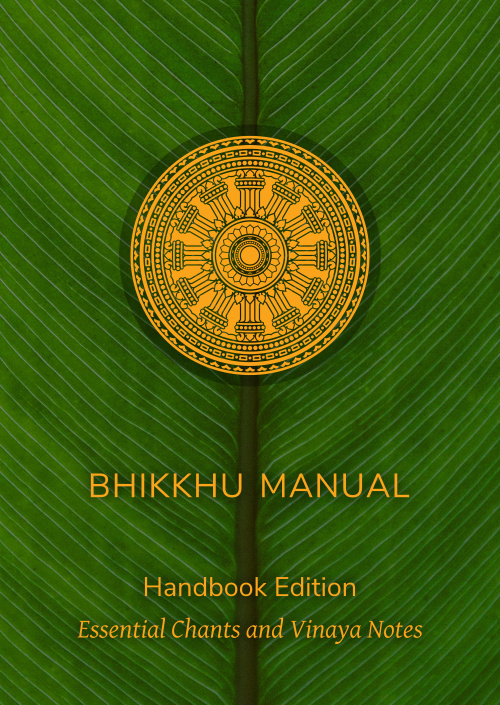
\includegraphics[height=\paperheight]{./handbook-desktop-cover.jpg}}
\fi

\cleartorecto
\thispagestyle{empty}
\vspace*{5em}

{\centering

\settowidth{\titleLength}{%
  {\Large\chapterTitleFont\scshape\MakeLowercase{\thetitle}}%
}

{\Large\chapterTitleFont\thetitle}\\[0.3\baselineskip]
\setlength{\xheight}{\heightof{X}}
\raisebox{0.5\xheight}{\color[gray]{0.4}\rule{\titleLength}{0.25pt}}\\[0.3\baselineskip]
{\itshape
\thesubtitle}

\vfill

\theauthor

\vspace*{5em}

}



\cleartoverso
\thispagestyle{empty}

{\copyrightsize
\centering
\setlength{\parindent}{0pt}%
\setlength{\parskip}{0.8\baselineskip}%

\thetitle\\
\thesubtitle

Published by \thePublisher

ISBN \theISBN

Copyright \copyright\ \thePublisher\ 2020

\vfill

{\footnotesize

This work is licensed under a Creative Commons\\
Attribution-NonCommercial-NoDerivatives 4.0 International~License.

Produced with the \LaTeX\ typesetting system,\\
set in Gentium and Nunito~Sans.

\theEditionInfo

}}


\cleartorecto
\thispagestyle{empty}

\mbox{}\vfill

{\centering\itshape

Namo tassa bhagavato arahato sammāsambuddhassa\\
Namo tassa bhagavato arahato sammāsambuddhassa\\
Namo tassa bhagavato arahato sammāsambuddhassa

}

\vfill\mbox{}

\vspace*{5\baselineskip}



\clearpage
{\subsectionFmt{Abbreviations used in the text}}
\bigskip

TODO: reformat references to accord with this

\bigskip

\begin{tabular}{@{}ll ll@{}}
  AN & Aṅguttara Nikāya & Pr & Pārājika\\
  Cv & Cullavagga &       Pv & Parivāra\\
  Dhp & Dhammapada &      SN & Saṃyutta Nikāya \\
  DN & Digha Nikāya  &    Sn & Sutta Nipāta\\
  It & Itivuttaka &       Th & Theragāthā \\
  Ja & Jātaka &           Thī & Therīgāthā\\
  Khp & Khuddakapāṭha &   Ud & Udāna\\
  MN & Majjhima Nikāya &  Vin & Vinaya Piṭaka\\
  Mv & Mahāvagga &        Vin-a & Vinaya Aṭṭhakathā\\
  Paṭis & Paṭisambhidā &  Vism & Visuddhimagga\\
\end{tabular}

\bigskip

{\subsectionFmt{Looking up references}}
\bigskip

TODO: Add instructions on how to look up references.



\cleartorecto
\pagestyle{toponerow-frontmatter}
\tableofcontents*

\clearpage
\listfirstlines*

\mainmatter
\pagestyle{toponerow}

\cleartorecto
\part{Essential Chants}

{\raggedright

\chapter{Morning Chanting}

\section*{Dedication of Offerings}

[Yo so] bhagavā arahaṃ sammāsambuddho\\
Svākkhāto yena bhagavatā dhammo\\
Supaṭipanno yassa bhagavato sāvakasaṅgho\\
Tam-mayaṃ bhagavantaṃ sadhammaṃ sasaṅghaṃ\\
Imehi sakkārehi yathārahaṃ āropitehi abhipūjayāma\\
Sādhu no bhante bhagavā sucira-parinibbutopi\\
Pacchimā-janatānukampa-mānasā\\
Ime sakkāre duggata-paṇṇākāra-bhūte paṭiggaṇhātu\\
Amhākaṃ dīgharattaṃ hitāya sukhāya\\
Arahaṃ sammāsambuddho bhagavā\\
Buddhaṃ bhagavantaṃ abhivādemi\\\relax
[Svākkhāto] bhagavatā dhammo\\
Dhammaṃ namassāmi\\\relax
[Supaṭipanno] bhagavato sāvakasaṅgho\\
Saṅghaṃ namāmi

[Yam-amha kho mayaṃ bhagavantaṃ saraṇaṃ gatā, uddissa pabbajitā yo no bhagavā
satthā, yassa ca mayaṃ bhagavato dhammaṃ rocema

Imehi sakkārehi taṃ bhagavantaṃ sasaddhammaṃ sasāvakasaṅghaṃ abhipūjayāma.]

\section*{Preliminary Homage}

\begin{leader}
  [Handa mayaṃ buddhassa bhagavato pubbabhāga-namakāraṃ karomase]
\end{leader}

Namo tassa bhagavato arahato sammāsambuddhassa (×3)

\section*{Homage to the Buddha}

\begin{leader}
  [Handa mayaṃ buddhābhitthutiṃ karomase]
\end{leader}

Yo so tathāgato arahaṃ sammāsambuddho\\
Vijjācaraṇa-sampanno, sugato, lokavidū\\
Anuttaro purisadamma-sārathi\\
Satthā deva-manussānaṃ, buddho bhagavā.

Yo imaṃ lokaṃ sadevakaṃ samārakaṃ sabrahmakaṃ\\
Sassamaṇa-brāhmaṇiṃ pajaṃ sadeva-manussaṃ sayaṃ abhiññā sacchikatvā pavedesi\\
Yo dhammaṃ desesi ādi-kalyāṇaṃ majjhe-kalyāṇaṃ pariyosāna-kalyāṇaṃ\\
Sātthaṃ sabyañjanaṃ kevala-paripuṇṇaṃ parisuddhaṃ brahma-cariyaṃ pakāsesi\\
Tam-ahaṃ bhagavantaṃ abhipūjayāmi tam-ahaṃ bhagavantaṃ sirasā namāmi

\section*{Homage to the Dhamma}

\begin{leader}
  [Handa mayaṃ dhammābhitthutiṃ karomase]
\end{leader}

Yo so svākkhāto bhagavatā dhammo\\
Sandiṭṭhiko, akāliko, ehipassiko, opanayiko\\
Paccattaṃ veditabbo viññūhi\\
Tam-ahaṃ dhammaṃ abhipūjayāmi tam-ahaṃ dhammaṃ sirasā namāmi

\section*{Homage to the Saṅgha}

\begin{leader}
  [Handa mayaṃ saṅghābhitthutiṃ karomase]
\end{leader}

Yo so supaṭipanno bhagavato sāvakasaṅgho\\
Ujupaṭipanno bhagavato sāvakasaṅgho\\
Ñāyapaṭipanno bhagavato sāvakasaṅgho\\
Sāmīcipaṭipanno bhagavato sāvakasaṅgho\\
Yadidaṃ cattāri purisayugāni aṭṭha purisapuggalā\\
Esa bhagavato sāvakasaṅgho\\
Āhuneyyo, pāhuneyyo, dakkhiṇeyyo, añjali-karaṇīyo\\
Anuttaraṃ puññakkhettaṃ lokassa\\
Tam-ahaṃ saṅghaṃ abhipūjayāmi tam-ahaṃ saṅghaṃ sirasā namāmi

\section*{Salutation to the Triple Gem}

\begin{leader}
  [Handa mayaṃ ratanattaya-paṇāma-gāthāyo c'eva\\
  saṃvega-parikittana-pāṭhañca bhaṇāmase]
\end{leader}

\firstline{Buddho susuddho karuṇā-mahaṇṇavo}

Buddho susuddho karuṇā-mahaṇṇavo\\
Yo'ccanta-suddhabbara-ñāṇa-locano\\
Lokassa pāpūpakilesa-ghātako\\
Vandāmi buddhaṃ aham-ādarena taṃ\\
Dhammo padīpo viya tassa satthuno\\
Yo magga-pākāmata-bheda-bhinnako\\
Lokuttaro yo ca tad-attha-dīpano\\
Vandāmi dhammaṃ aham-ādarena taṃ\\
Saṅgho sukhettābhyati-khetta-saññito\\
Yo diṭṭha-santo sugatānubodhako\\
Lolappahīno ariyo sumedhaso\\
Vandāmi saṅghaṃ aham-ādarena taṃ\\
Iccevam-ekantabhipūja-neyyakaṃ vatthuttayaṃ \\vandayatābhisaṅkhataṃ\\
Puññaṃ mayā yaṃ mama sabbupaddavā mā hontu ve tassa pabhāva-siddhiyā

Idha tathāgato loke uppanno arahaṃ sammāsambuddho\\
Dhammo ca desito niyyāniko upasamiko parinibbāniko sambodhagāmī sugatappavedito\\
Mayan-taṃ dhammaṃ sutvā evaṃ jānāma

Jātipi dukkhā\\
Jarāpi dukkhā\\
Maraṇampi dukkhaṃ\\
Soka-parideva-dukkha-domanass'upāyāsāpi dukkhā\\
Appiyehi sampayogo dukkho\\
Piyehi vippayogo dukkho\\
Yamp'icchaṃ na labhati tampi dukkhaṃ\\
Saṅkhittena pañcupādānakkhandhā dukkhā

Seyyathīdaṃ\\
Rūpūpādānakkhandho\\
Vedanūpādānakkhandho\\
Saññūpādānakkhandho\\
Saṅkhārūpādānakkhandho\\
Viññāṇūpādānakkhandho

Yesaṃ pariññāya\\
Dharamāno so bhagavā evaṃ bahulaṃ sāvake vineti\\
Evaṃ bhāgā ca panassa bhagavato sāvakesu anusāsanī bahulā pavattati

Rūpaṃ aniccaṃ\\
Vedanā aniccā\\
Saññā aniccā\\
Saṅkhārā aniccā\\
Viññāṇaṃ aniccaṃ\\
Rūpaṃ anattā\\
Vedanā anattā\\
Saññā anattā\\
Saṅkhārā anattā\\
Viññāṇaṃ anattā\\
Sabbe saṅkhārā aniccā\\
Sabbe dhammā anattā'ti

Te mayaṃ otiṇṇāmha jātiyā jarā-maraṇena\\
Sokehi paridevehi dukkhehi domanassehi upāyāsehi\\
Dukkhotiṇṇā dukkha-paretā\\
Appeva nāmimassa kevalassa dukkha-kkhandhassa\\
antakiriyā paññāyethā'ti

Cira-parinibbutampi taṃ bhagavantaṃ uddissa arahantaṃ sammāsambuddhaṃ\\
Saddhā agārasmā anagāriyaṃ pabbajitā\\
Tasmiṃ bhagavati brahma-cariyaṃ carāma\\
Bhikkhūnaṃ/Sīladharānaṃ sikkhāsājīva-samāpannā\\
Taṃ no brahma-cariyaṃ imassa kevalassa dukkha-kkhandhassa antakiriyāya saṃvattatu

\enlargethispage{\baselineskip}

\section*{Closing Homage}

[Arahaṃ] sammāsambuddho bhagavā\\
Buddhaṃ bhagavantaṃ abhivādemi

[Svākkhāto] bhagavatā dhammo\\
Dhammaṃ namassāmi

[Supaṭipanno] bhagavato sāvakasaṅgho\\
Saṅghaṃ namāmi


\chapter{Evening Chanting}

\section*{Dedication of Offerings}

\firstline{Yo so bhagavā arahaṃ sammāsambuddho}

[Yo so] bhagavā arahaṃ sammāsambuddho\\
Svākkhāto yena bhagavatā dhammo\\
Supaṭipanno yassa bhagavato sāvakasaṅgho\\
Tam-mayaṃ bhagavantaṃ sadhammaṃ sasaṅghaṃ\\
Imehi sakkārehi yathārahaṃ āropitehi abhipūjayāma\\
Sādhu no bhante bhagavā sucira-parinibbutopi\\
Pacchimā-janatānukampa-mānasā\\
Ime sakkāre duggata-paṇṇākāra-bhūte paṭiggaṇhātu\\
Amhākaṃ dīgharattaṃ hitāya sukhāya\\
Arahaṃ sammāsambuddho bhagavā\\
Buddhaṃ bhagavantaṃ abhivādemi

[Svākkhāto] bhagavatā dhammo\\
Dhammaṃ namassāmi

[Supaṭipanno] bhagavato sāvakasaṅgho\\
Saṅghaṃ namāmi

[Yam-amha kho mayaṃ bhagavantaṃ saraṇaṃ gatā, uddissa pabbajitā yo no bhagavā
satthā, yassa ca mayaṃ bhagavato dhammaṃ rocema

Imehi sakkārehi taṃ bhagavantaṃ sasaddhammaṃ sasāvaka-saṅghaṃ abhipūjayāma.]

\section*{Preliminary Homage}

\begin{leader}
  [Handa mayaṃ buddhassa bhagavato pubbabhāga-namakāraṃ karomase]
\end{leader}

Namo tassa bhagavato arahato sammāsambuddhassa (×3)

\section*{Recollection of the Buddha}

\begin{leader}
  [Handa mayaṃ buddhānussatinayaṃ karomase]
\end{leader}

Taṃ kho pana bhagavantaṃ evaṃ kalyāṇo\\
\vin kittisaddo abbhuggato\\
Itipi so bhagavā arahaṃ sammāsambuddho\\
Vijjācaraṇa-sampanno sugato lokavidū\\
Anuttaro purisadamma-sārathi satthā deva-manussānaṃ\\
\vin buddho bhagavā'ti

\section*{Supreme Praise of the Buddha}

\begin{leader}
  [Handa mayaṃ buddhābhigītiṃ karomase]
\end{leader}

Buddh'vārahanta-varatādiguṇābhiyutto\\
Suddhābhiñāṇa-karuṇāhi samāgatatto\\
Bodhesi yo sujanataṃ kamalaṃ va sūro\\
Vandām'ahaṃ tam-araṇaṃ sirasā jinendaṃ\\
Buddho yo sabba-pāṇīnaṃ saraṇaṃ khemam-uttamaṃ\\
Paṭhamānussatiṭṭhānaṃ vandāmi taṃ siren'ahaṃ\\
Buddhassāh'asmi dāso/dāsī va buddho me sāmi-kissaro\\
Buddho dukkhassa ghātā ca vidhātā ca hitassa me\\
Buddhass'āhaṃ niyyādemi sarīrañ-jīvitañ-cidaṃ\\
Vandanto'haṃ/Vandantī'haṃ carissāmi\\
\vin buddhass'eva subodhitaṃ\\
Natthi me saraṇaṃ aññaṃ buddho me saraṇaṃ varaṃ\\
Etena sacca-vajjena vaḍḍheyyaṃ satthu-sāsane\\
Buddhaṃ me vandamānena/vandamānāya\\
\vin yaṃ puññaṃ pasutaṃ idha\\
Sabbepi antarāyā me māhesuṃ tassa tejasā

\enlargethispage{\baselineskip}

\instr{(Bowing)}

Kāyena vācāya va cetasā vā\\
Buddhe kukammaṃ pakataṃ mayā yaṃ\\
Buddho paṭiggaṇhātu accayantaṃ\\
Kālantare saṃvarituṃ va buddhe

\section*{Recollection of the Dhamma}

\begin{leader}
  [Handa mayaṃ dhammānussatinayaṃ karomase]
\end{leader}

Svākkhāto bhagavatā dhammo\\
Sandiṭṭhiko akāliko ehipassiko\\
Opanayiko paccattaṃ veditabbo viññūhī'ti

\section*{Supreme Praise of the Dhamma}

\begin{leader}
  [Handa mayaṃ dhammābhigītiṃ karomase]
\end{leader}

Svākkhātat'ādiguṇa-yoga-vasena seyyo\\
Yo magga-pāka-pariyatti-vimokkha-bhedo\\
Dhammo kuloka-patanā tada-dhāri-dhārī\\
Vandām'ahaṃ tama-haraṃ vara-dhammam-etaṃ\\
Dhammo yo sabba-pāṇīnaṃ saraṇaṃ khemam-uttamaṃ\\
Dutiyānussatiṭṭhānaṃ vandāmi taṃ siren'ahaṃ\\
Dhammassāh'asmi dāso/dāsī va dhammo me sāmi-kissaro\\
Dhammo dukkhassa ghātā ca vidhātā ca hitassa me\\
Dhammass'āhaṃ niyyādemi sarīrañ-jīvitañ-cidaṃ\\
Vandantohaṃ/Vandantīhaṃ carissāmi\\
\vin dhammass'eva sudhammataṃ\\
Natthi me saraṇaṃ aññaṃ dhammo me saraṇaṃ varaṃ\\
Etena sacca-vajjena vaḍḍheyyaṃ satthu-sāsane\\
Dhammaṃ me vandamānena/vandamānāya\\
\vin yaṃ puññaṃ pasutaṃ idha\\
Sabbepi antarāyā me māhesuṃ tassa tejasā

\instr{(Bowing)}

Kāyena vācāya va cetasā vā\\
Dhamme kukammaṃ pakataṃ mayā yaṃ\\
Dhammo paṭiggaṇhātu accayantaṃ\\
Kālantare saṃvarituṃ va dhamme

\section*{Recollection of the Saṅgha}

\begin{leader}
  [Handa mayaṃ saṅghānussatinayaṃ karomase]
\end{leader}

Supaṭipanno bhagavato sāvakasaṅgho\\
Ujupaṭipanno bhagavato sāvakasaṅgho\\
Ñāyapaṭipanno bhagavato sāvakasaṅgho\\
Sāmīcipaṭipanno bhagavato sāvakasaṅgho\\
Yadidaṃ cattāri purisayugāni aṭṭha purisapuggalā\\
Esa bhagavato sāvakasaṅgho\\
Āhuneyyo pāhuneyyo dakkhiṇeyyo añjali-karaṇīyo\\
Anuttaraṃ puññakkhettaṃ lokassā'ti

\clearpage

\section*{Supreme Praise of the Saṅgha}

\begin{leader}
  [Handa mayaṃ saṅghābhigītiṃ karomase]
\end{leader}

Saddhammajo supaṭipatti-guṇādiyutto\\
Yo'ṭṭhabbidho ariyapuggala-saṅgha-seṭṭho\\
Sīlādidhamma-pavarāsaya-kāya-citto\\
Vandām'ahaṃ tam-ariyāna-gaṇaṃ susuddhaṃ\\
Saṅgho yo sabba-pāṇīnaṃ saraṇaṃ khemam-uttamaṃ\\
Tatiyānussatiṭṭhānaṃ vandāmi taṃ siren'ahaṃ\\
Saṅghass'āhasmi dāso/dāsī va saṅgho me sāmi-kissaro\\
Saṅgho dukkhassa ghātā ca vidhātā ca hitassa me\\
Saṅghass'āhaṃ niyyādemi sarīrañ-jīvitañ-cidaṃ\\
Vandanto'haṃ/Vandantī'haṃ carissāmi\\
\vin saṅghassopaṭipannataṃ\\
Natthi me saraṇaṃ aññaṃ saṅgho me saraṇaṃ varaṃ\\
Etena sacca-vajjena vaḍḍheyyaṃ satthu-sāsane\\
Saṅghaṃ me vandamānena/vandamānāya\\
\vin yaṃ puññaṃ pasutaṃ idha\\
Sabbepi antarāyā me māhesuṃ tassa tejasā

\enlargethispage{\baselineskip}

\instr{(Bowing)}

Kāyena vācāya va cetasā vā\\
Saṅghe kukammaṃ pakataṃ mayā yaṃ\\
Saṅgho paṭiggaṇhātu accayantaṃ\\
Kālantare saṃvarituṃ va saṅghe

\section*{Closing Homage}

[Arahaṃ] sammāsambuddho bhagavā\\
Buddhaṃ bhagavantaṃ abhivādemi

[Svākkhāto] bhagavatā dhammo\\
Dhammaṃ namassāmi

[Supaṭipanno] bhagavato sāvakasaṅgho\\
Saṅghaṃ namāmi


\chapter{Reflections}

\section{Reflection on the Four Requisites}

\begin{leader}
  [Handa mayaṃ taṅkhaṇika-\\ paccavekkhaṇa-pāṭhaṃ bhaṇāmase]
\end{leader}

\firstline{Paṭisaṅkhā yoniso cīvaraṃ paṭisevāmi}

[Paṭisaṅkhā] yoniso cīvaraṃ paṭisevāmi,\\
yāvadeva sītassa paṭighātāya, uṇhassa paṭighātāya,\\
ḍaṃsa-makasa-vātātapa-siriṃsapa-samphassānaṃ\\
paṭighātāya, yāvadeva hirikopina-paṭicchādanatthaṃ

\begin{english}
  Wisely reflecting, I use the robe: only to ward off cold, to ward off heat, to
  ward off the touch of flies, mosquitoes, wind, burning and creeping things,
  only for the sake of modesty.
\end{english}

[Paṭisaṅkhā] yoniso piṇḍapātaṃ paṭisevāmi, neva davāya, na madāya, na maṇḍanāya,
na vibhūsanāya, yāvadeva imassa kāyassa ṭhitiyā, yāpanāya, vihiṃsūparatiyā,
brahmacariyānuggahāya, iti purāṇañca vedanaṃ paṭihaṅkhāmi, navañca vedanaṃ na
uppādessāmi, yātrā ca me bhavissati anavajjatā ca phāsuvihāro cā'ti

\begin{english}
  Wisely reflecting, I use almsfood: not for fun, not for pleasure, not for
  fattening, not for beautification, only for the maintenance and nourishment of
  this body, for keeping it healthy, for helping with the Holy Life; thinking
  thus, `I will allay hunger without overeating, so that I may continue to live
  blamelessly and at ease.'
\end{english}

[Paṭisaṅkhā] yoniso senāsanaṃ paṭisevāmi,\\
yāvadeva sītassa paṭighātāya, uṇhassa paṭighātāya,\\
ḍaṃsa-makasa-vātātapa-siriṃsapa-samphassānaṃ\\
paṭighātāya, yāvadeva utuparissaya vinodanaṃ paṭisallānārāmatthaṃ

\begin{english}
  Wisely reflecting, I use the lodging: only to ward off cold, to ward off heat,
  to ward off the touch of flies, mosquitoes, wind, burning and creeping things,
  only to remove the danger from weather, and for living in seclusion.
\end{english}

[Paṭisaṅkhā] yoniso gilāna-paccaya-bhesajja-parikkhāraṃ paṭisevāmi, yāvadeva
uppannānaṃ veyyābādhikānaṃ vedanānaṃ paṭighātāya, abyāpajjha-paramatāyā'ti

\begin{english}
  Wisely reflecting, I use supports for the sick and medicinal requisites: only
  to ward off painful feelings that have arisen, for the maximum freedom from
  disease.
\end{english}

\suttaRef{M.I.10}

\section{Five Subjects for Frequent Recollection}

\begin{leader}
  [Handa mayaṃ abhiṇha-paccavekkhaṇa-pāṭhaṃ bhaṇāmase]
\end{leader}

\firstline{Jarā-dhammomhi jaraṃ anatīto}

\instr{(Men Chant)}

[Jarā-dhammomhi] jaraṃ anatīto

\begin{english}
  I am of the nature to age, I have not gone beyond ageing.
\end{english}

Byādhi-dhammomhi byādhiṃ anatīto

\begin{english}
  I am of the nature to sicken, I have not gone beyond sickness.
\end{english}

Maraṇa-dhammomhi maraṇaṃ anatīto

\begin{english}
  I am of the nature to die, I have not gone beyond dying.
\end{english}

Sabbehi me piyehi manāpehi nānābhāvo vinābhāvo

\begin{english}
  All that is mine, beloved and pleasing,\\
  will become otherwise, will become separated from me.
\end{english}

Kammassakomhi kammadāyādo kammayoni kammabandhu kammapaṭisaraṇo\\
Yaṃ kammaṃ karissāmi, kalyāṇaṃ vā pāpakaṃ vā, tassa dāyādo bhavissāmi

\begin{english}
  I am the owner of my kamma, heir to my kamma, born of my kamma,\\
  related to my kamma, abide supported by my kamma.\\
  Whatever kamma I shall do, for good or for ill, of \prul{that} I will be the heir.
\end{english}

Evaṃ amhehi abhiṇhaṃ paccavekkhitabbaṃ

\begin{english}
  \prul{Thus} we should frequently recollect.
\end{english}

\instr{(Women Chant)}

[Jarā-dhammāmhi] jaraṃ anatītā

\begin{english}
  I am of the nature to age, I have not gone beyond ageing.
\end{english}

Byādhi-dhammāmhi byādhiṃ anatītā

\begin{english}
  I am of the nature to sicken, I have not gone beyond sickness.
\end{english}

Maraṇa-dhammāmhi maraṇaṃ anatītā

\begin{english}
  I am of the nature to die, I have not gone beyond dying.
\end{english}

Sabbehi me piyehi manāpehi nānābhāvo vinābhāvo

\begin{english}
  All that is mine, beloved and pleasing,\\
  will become otherwise, will become separated from me.
\end{english}

Kammassakāmhi kammadāyādā kammayoni kammabandhu kammapaṭisaraṇā\\
Yaṃ kammaṃ karissāmi, kalyāṇaṃ vā pāpakaṃ vā, tassa dāyādā bhavissāmi

\begin{english}
  I am the owner of my kamma, heir to my kamma, born of my kamma,\\
  related to my kamma, abide supported by my kamma.\\
  Whatever kamma I shall do, for good or for ill, of \prul{that} I will be the heir.
\end{english}

Evaṃ amhehi abhiṇhaṃ paccavekkhitabbaṃ

\begin{english}
  \prul{Thus} we should frequently recollect.
\end{english}

\suttaRef{A.III.71}

\section{Ten Subjects for Frequent Recollection}

\firstline{Dasa ime bhikkhave}

\begin{leader}
  [Handa mayaṃ pabbajita\hyp{}abhiṇha-\\ paccavekkhaṇa\hyp{}pāṭhaṃ bhaṇāmase]
\end{leader}

[Dasa ime bhikkhave] dhammā pabbajitena abhiṇhaṃ paccavekkhitabbā, katame dasa

\begin{english}
  Bhikkhus, there are ten dhammas which should be reflected upon, again and again, by one who has gone forth. \prul{What} are these ten?
\end{english}

Vevaṇṇiyamhi ajjhūpagato'ti pabbajitena abhiṇhaṃ paccavekkhitabbaṃ

\begin{english}
  `I am no longer living according to worldly aims and values.'\\
  This should be reflected upon, again and again,\\
  by one who has gone forth.
\end{english}

Parapaṭibaddhā me jīvikā'ti pabbajitena abhiṇhaṃ paccavekkhitabbaṃ

\begin{english}
  `My very life is sustained through the gifts of others.'\\
  This should be reflected upon, again and again,\\
  by one who has gone forth.
\end{english}

Añño me ākappo karaṇīyo'ti pabbajitena abhiṇhaṃ paccavekkhitabbaṃ

\begin{english}
  `I should strive to abandon my former habits.'\\
  This should be reflected upon, again and again,\\
  by one who has gone forth.
\end{english}

Kacci nu kho me attā sīlato na upavadatī'ti pabbajitena abhiṇhaṃ paccavekkhitabbaṃ

\begin{english}
  `Does regret over my conduct arise in my mind?'\\
  This should be reflected upon, again and again,\\
  by one who has gone forth.
\end{english}

Kacci nu kho maṃ anuvicca viññū sabrahmacārī sīlato na upavadantī'ti pabbajitena abhiṇhaṃ paccavekkhitabbaṃ

\begin{english}
  `Could my spiritual companions find fault with my conduct?'\\
  This should be reflected upon, again and again,\\
  by one who has gone forth.
\end{english}

Sabbehi me piyehi manāpehi nānābhāvo vinābhāvo'ti pabbajitena abhiṇhaṃ paccavekkhitabbaṃ

\begin{english}
  `All that is mine, beloved and pleasing, will become otherwise, will become separated from me.'\\
  This should be reflected upon, again and again,\\
  by one who has gone forth.
\end{english}

Kammassakomhi kammadāyādo kammayoni kammabandhu kammapaṭisaraṇo, yaṃ kammaṃ karissāmi, kalyāṇaṃ vā pāpakaṃ vā, tassa dāyādo bhavissāmī'ti pabbajitena abhiṇhaṃ paccavekkhitabbaṃ

\begin{english}
  `I am the owner of my kamma, heir to my kamma,\\
  born of my kamma, related to my kamma,\\
  abide supported by my kamma; whatever kamma I shall do,\\
  for good or for ill, of \prul{that} I will be the heir.'\\
  This should be reflected upon, again and again,\\
  by one who has gone forth.
\end{english}

`Kathambhūtassa me rattindivā vītipatantī'ti pabbajitena abhiṇhaṃ paccavekkhitabbaṃ

\begin{english}
  `The days and nights are relentlessly passing; how well am I spending my time?'\\
  This should be reflected upon, again and again,\\
  by one who has gone forth.
\end{english}

Kacci nu kho'haṃ suññāgāre abhiramāmī'ti pabbajitena abhiṇhaṃ paccavekkhitabbaṃ

\begin{english}
  `Do I delight in solitude or not?'\\
  This should be reflected upon, again and again,\\
  by one who has gone forth.
\end{english}

Atthi nu kho me uttari-manussa-dhammā alamariya-ñāṇa-dassana-viseso adhigato, so'haṃ pacchime kāle sabrahmacārīhi puṭṭho na maṅku bhavissāmī'ti pabbajitena abhiṇhaṃ paccavekkhitabbaṃ

\begin{english}
  `Has my practice borne fruit with freedom or insight so that at the end of my life I need not feel ashamed when questioned by my spiritual companions?'\\
  This should be reflected upon, again and again,\\
  by one who has gone forth.
\end{english}

Ime kho bhikkhave dasa dhammā pabbajitena abhiṇhaṃ paccavekkhitabbā'ti

\begin{english}
  Bhikkhus, these are the ten dhammas to be reflected upon, again and again, by one who has gone forth.
\end{english}

\suttaRef{A.V.87}

\section{Caturappamaññā-obhāsanaṃ}

\firstline{Mettā-sahagatena}

\begin{leader}
  [Handa mayaṃ caturappamaññā-obhāsanaṃ karomase]
\end{leader}

[Mettā-sahagatena] cetasā ekaṃ disaṃ pharitvā viharati\\
Tathā dutiyaṃ tathā tatiyaṃ tathā catutthaṃ\\
Iti uddhamadho tiriyaṃ sabbadhi sabbattatāya\\
Sabbāvantaṃ lokaṃ mettā-sahagatena cetasā\\
Vipulena mahaggatena appamāṇena averena abyāpajjhena\\
\vin pharitvā viharati

Karuṇā-sahagatena cetasā ekaṃ disaṃ pharitvā viharati\\
Tathā dutiyaṃ tathā tatiyaṃ tathā catutthaṃ\\
Iti uddhamadho tiriyaṃ sabbadhi sabbattatāya\\
Sabbāvantaṃ lokaṃ karuṇā-sahagatena cetasā\\
Vipulena mahaggatena appamāṇena averena abyāpajjhena\\
\vin pharitvā viharati

Muditā-sahagatena cetasā ekaṃ disaṃ pharitvā viharati\\
Tathā dutiyaṃ tathā tatiyaṃ tathā catutthaṃ\\
Iti uddhamadho tiriyaṃ sabbadhi sabbattatāya\\
Sabbāvantaṃ lokaṃ muditā-sahagatena cetasā\\
Vipulena mahaggatena appamāṇena averena abyāpajjhena\\
\vin pharitvā viharati

Upekkhā-sahagatena cetasā ekaṃ disaṃ pharitvā viharati\\
Tathā dutiyaṃ tathā tatiyaṃ tathā catutthaṃ\\
Iti uddhamadho tiriyaṃ sabbadhi sabbattatāya\\
Sabbāvantaṃ lokaṃ upekkhā-sahagatena cetasā\\
Vipulena mahaggatena appamāṇena averena abyāpajjhena\\
\vin pharitvā viharatī'ti

\suttaRef{D.I.251}

\subsubsection{Suffusion With the Divine Abidings}

\firstline{I will abide}

\begin{leader}
  [Now let us make the Four Boundless Qualities shine forth.]
\end{leader}

[\prul{I} will abide] pervading one quarter with a heart imbued\\
\vin with loving-kindness;\\
Likewise the second, likewise the third, likewise the fourth;\\
So above and below, around and everywhere; and to \prul{all} as to myself.\\
\prul{I} will abide pervading the all-encompassing world with a heart \\
\vin imbued with loving-kindness; abundant, exalted,\\
\vin immeasurable, without hostility, and without ill-will.

\prul{I} will abide pervading one quarter with a heart imbued\\
\vin with compassion;\\
Likewise the second, likewise the third, likewise the fourth;\\
So above and below, around and everywhere; and to \prul{all} as to myself.\\
\prul{I} will abide pervading the all-encompassing world with a heart \\
\vin imbued with compassion; abundant, exalted,\\
\vin immeasurable, without hostility, and without ill-will.

\prul{I} will abide pervading one quarter with a heart imbued\\
\vin with gladness;\\
Likewise the second, likewise the third, likewise the fourth;\\
So above and below, around and everywhere; and to \prul{all} as to myself.\\
\prul{I} will abide pervading the all-encompassing world with a heart \\
\vin imbued with gladness; abundant, exalted,\\
\vin immeasurable, without hostility, and without ill-will.

\prul{I} will abide pervading one quarter with a heart imbued\\
\vin with equanimity;\\
Likewise the second, likewise the third, likewise the fourth;\\
So above and below, around and everywhere; and to \prul{all} as to myself.\\
\prul{I} will abide pervading the all-encompassing world with a heart \\
\vin imbued with equanimity; abundant, exalted,\\
\vin immeasurable, without hostility, and without ill-will.

\section{Dedication of Merit to the Devas and Others}

% Pali title: Devatādi-patti-dāna-gāthā

% Gavesako: I have only done this chant at Dhammayut monasteries. Is it necessary?

\begin{leader}
  [Handa mayaṃ patti-dāna-gāthāyo bhaṇāmase]
\end{leader}

\firstline{Yā devatā santi vihāra-vāsinī}

\enlargethispage{\baselineskip}

Yā devatā santi vihāra-vāsinī\\
Thūpe ghare bodhi-ghare tahiṃ tahiṃ\\
Tā dhamma-dānena bhavantu pūjitā\\
Sotthiṃ karonte'dha vihāra-maṇḍale.\\
Therā ca majjhā navakā ca bhikkhavo\\
Sārāmikā dāna-patī upāsakā\\
Gāmā ca desā nigamā ca issarā\\
Sappāṇa-bhūtā sukhitā bhavantu te.\\
Jalābu-jā ye pi ca aṇḍa-sambhavā\\
Saṃseda-jātā atha-v-opapātikā\\
Niyyānikaṃ dhamma-varaṃ paṭicca te\\
Sabbe pi dukkhassa karontu saṅkhayaṃ.\\
Ṭhātu ciraṃ sataṃ dhammo\\
Dhamma-dharā ca puggalā\\
Saṅgho hotu samaggo va\\
Atthāya ca hitāya ca\\
Amhe rakkhatu saddhammo\\
Sabbe pi dhamma-cārino\\
Vuḍḍhiṃ sampāpuṇeyyāma\\
Dhamme ariyappavedite.

\subsubsection{Pasannā hontu sabbe pi}

% Gavesako: I have only done this chant at Dhammayut monasteries. Is it necessary?

\firstline{Pasannā hontu sabbe pi}

Pasannā hontu sabbe pi\\
Pāṇino Buddha-sāsane.\\
Sammā-dhāraṃ pavecchanto\\
Kāle devo pavassatu.\\
Vuḍḍhi-bhāvāya sattānaṃ\\
Samiddhaṃ netu medaniṃ.\\
Mātā-pitā ca atra-jaṃ\\
Niccaṃ rakkhanti puttakaṃ.\\
Evaṃ dhammena rājāno\\
Pajaṃ rakkhantu sabbadā.

\section{Recollection After Using the Requisites}
\label{recollection-after-using}

\begin{leader}
  [Handa mayaṃ atīta-paccavekkhaṇa-pāṭhaṃ bhaṇāmase]
\end{leader}

\firstline{Ajja mayā apaccavekkhitvā yaṃ cīvaraṃ}

Ajja mayā apaccavekkhitvā yaṃ cīvaraṃ paribhuttaṃ,\\
taṃ yāvadeva sītassa paṭighātāya, uṇhassa paṭighātāya,\\
ḍaṃsa-makasa-vātātapa-siriṃsapa-samphassānaṃ\\
paṭighātāya, yāvadeva hirikopina paṭicchādan'atthaṃ.

\begin{english}
  Whatever robe I used today without consideration,\\
  Was only to ward off cold,\\
  to ward off heat,\\
  to ward off the touch of flies, mosquitoes, wind, burning and creeping things,\\
  only for the sake of modesty.
\end{english}

Ajja mayā apaccavekkhitvā yo piṇḍapāto paribhutto, so n'eva davāya, na madāya, na
maṇḍanāya, na vibhūsanāya, yāvad-eva imassa kāyassa ṭhitiyā, yāpanāya,
vihiṃsūparatiyā, brahmacariyānuggahāya, iti purāṇañca vedanaṃ paṭihaṅkhāmi,
navañca vedanaṃ na uppādessāmi, yātrā ca me bhavissati anavajjatā ca
phāsuvihāro cā'ti.

\begin{english}
  Whatever alms-food I used today without consideration,\\
  was not for fun, not for pleasure, not for fattening, not for beautification,\\
  only for the maintenance and nourishment of this body, for keeping it healthy, for helping with the Holy Life;\\
  thinking thus, `I will allay hunger without overeating, so that I may continue to live blamelessly and at ease.'
\end{english}

Ajja mayā apaccavekkhitvā yaṃ senāsanaṃ paribhuttaṃ, taṃ yāvadeva sītassa
paṭighātāya, uṇhassa paṭighātāya, ḍaṃsa-makasa-vātātapa-siriṃsapa-samphassānaṃ
paṭighātāya, yāvadeva utuparissaya vinodanaṃ paṭisallānārāmatthaṃ.

\begin{english}
  Whatever lodging I used today without consideration,\\
  was only to ward off cold,\\
  to ward off heat,\\
  to ward off the touch of flies, mosquitoes, wind, burning and creeping things,\\
  only to remove the danger from weather, and for living in seclusion.
\end{english}

Ajja mayā apaccavekkhitvā yo gilāna-paccayabhesajja-\\ parikkhāro paribhutto, so
yāvadeva uppannānaṃ veyyābādhikānaṃ vedanānaṃ paṭighātāya,\\
abyāpajjha-paramatāyā'ti.

\begin{english}
  Whatever medicinal requisite for supporting the sick I used today without consideration,\\
  was only to ward off painful feelings that have arisen,\\
  for the maximum freedom from disease.
\end{english}

\suttaRef{M.I.10}

\section[Reflection on the Off-Putting Qualities]{Reflection on the Off-Putting Qualities of the Requisites}

% Pali title: Dhātu-paṭikūla-paccavekkhaṇa-pāṭho

% This seems to be a modern compilation somewhat based on the MN 28 sub-commentary.

\begin{leader}
  [Handa mayaṃ dhātu-paṭikūla-\\ paccavekkhaṇa-pāṭhaṃ bhaṇāmase]
\end{leader}

\firstline{Yathā paccayaṃ pavattamānaṃ dhātu-mattam}

[Yathā paccayaṃ] pavattamānaṃ dhātu-mattam-ev'etaṃ

\trline{Composed of only elements according to causes and conditions}

Yad idaṃ cīvaraṃ tad upabhuñjako ca puggalo

\trline{Are these robes and so is the person wearing them;}

Dhātu-mattako, nissatto, nijjīvo, suñño

\trline{Merely elements, not a being, without a soul, and empty of self.}

Sabbāni pana imāni cīvarāni ajigucchanīyāni

\trline{None of these robes are innately repulsive}

Imaṃ pūti-kāyaṃ patvā, ativiya jigucchanīyāni jāyanti

\trline{But touching this unclean body, they become disgusting indeed.}

Yathā paccayaṃ pavattamānaṃ dhātu-mattam-ev'etaṃ

\trline{Composed of only elements according to causes and conditions}

Yad idaṃ piṇḍapāto tad upabhuñjako ca puggalo

\trline{Is this almsfood and so is the person eating it;}

Dhātu-mattako, nissatto, nijjīvo, suñño

\trline{Merely elements, not a being, without a soul, and empty of self.}

Sabbo panāyaṃ piṇḍapāto ajigucchanīyo

\trline{None of this almsfood is innately repulsive}

Imaṃ pūti-kāyaṃ patvā, ativiya jigucchanīyo jāyati

\trline{But touching this unclean body, it becomes disgusting indeed.}

Yathā paccayaṃ pavattamānaṃ dhātu-mattam-ev'etaṃ

\trline{Composed of only elements according to causes and conditions}

Yad idaṃ senāsanaṃ tad upabhuñjako ca puggalo

\trline{Is this dwelling and so is the person using it;}

Dhātu-mattako, nissatto, nijjīvo, suñño

\trline{Merely elements, not a being, without a soul, and empty of self.}

Sabbāni pana imāni senāsanāni ajigucchanīyāni

\trline{None of these dwellings are innately repulsive}

Imaṃ pūti-kāyaṃ patvā, ativiya jigucchanīyāni jāyanti

\trline{But touching this unclean body, they become disgusting indeed.}

Yathā paccayaṃ pavattamānaṃ dhātu-mattam-ev'etaṃ

\trline{Composed of only elements according to causes and conditions}

Yad idaṃ gilāna-paccaya-bhesajja-parikkhāro tad upabhuñjako ca puggalo

\trline{Is this medicinal requisite and so is the person that takes it;}

Dhātu-mattako, nissatto, nijjīvo, suñño

\trline{Merely elements, not a being, without a soul, and empty of self.}

Sabbo panāyaṃ gilāna-paccaya-bhesajja-parikkhāro ajigucchanīyo

\trline{None of this medicinal requisite is innately repulsive}

Imaṃ pūti-kāyaṃ patvā, ativiya jigucchanīyo jāyati

\trline{But touching this unclean body, it becomes disgusting indeed.}

\section{Mettāpharaṇaṃ}

\begin{leader}
  [Handa mayam mettāpharaṇaṃ karomase]
\end{leader}

\firstline{Ahaṃ sukhito homi niddukkho homi}

[Ahaṃ sukhito homi] niddukkho homi, avero homi, abyāpajjho homi, anīgho homi,
sukhī attānaṃ pariharāmi

Sabbe sattā sukhitā hontu, sabbe sattā averā hontu, sabbe sattā abyāpajjhā
hontu, sabbe sattā anīghā hontu, sabbe sattā sukhī attānaṃ pariharantu

Sabbe sattā sabbadukkhā pamuccantu

Sabbe sattā laddha-sampattito mā vigacchantu

Sabbe sattā kammassakā kammadāyādā kammayonī kammabandhū kammapaṭisaraṇā,
yaṃ kammaṃ karissanti, kalyāṇaṃ vā pāpakaṃ vā, tassa dāyādā bhavissanti

\suttaRef{M.I.288; A.V.88}

\subsubsection{Reflection on Universal Well-Being}

\begin{leader}
  [Now let us chant the reflections on universal well-being]
\end{leader}

\firstline{May I abide in well-being}

[May I abide in well-being,]\\
In freedom from affliction,\\
In freedom from hostility,\\
In freedom from ill-will,\\
In freedom from anxiety,\\
And may I maintain well-being in myself.

May everyone abide in well-being,\\
In freedom from hostility,\\
In freedom from ill-will,\\
In freedom from anxiety, and may they\\
Maintain well-being in themselves.

May all beings be released from all suffering.

And may they not be parted from the good fortune they have attained.

When they act upon intention,\\
All beings are the owners of their action and inherit its results.\\
Their future is born from such action,\\
companion to such action,\\
And its results will be their home.

All actions with intention,\\
Be they skilful or harmful ---\\
Of such acts they will be the heirs.

\suttaRef{M.I.288; A.V.88}

\section[The Unconditioned]{Reflection on the Unconditioned}

\begin{leader}
  [Handa mayaṃ nibbāna-sutta-pāṭhaṃ bhaṇāmase]
\end{leader}

\firstline{Atthi bhikkhave ajātaṃ abhūtaṃ akataṃ}

Atthi bhikkhave ajātaṃ abhūtaṃ akataṃ asaṅkhataṃ

\begin{english}
  There is an Unborn, Unoriginated, Uncreated and Unformed.
\end{english}

No cetaṃ bhikkhave abhavissa ajātaṃ abhūtaṃ akataṃ asaṅkhataṃ

\begin{english}
  If there was not this Unborn, this Unoriginated, this Uncreated, this~Unformed,
\end{english}

Na yidaṃ jātassa bhūtassa katassa saṅkhatassa nissaraṇaṃ paññāyetha

\begin{english}
  Freedom from the world of the born, the originated, the created, the formed would not be possible.
\end{english}

Yasmā ca kho bhikkhave atthi ajātaṃ abhūtaṃ akataṃ asaṅkhataṃ

\begin{english}
  But since there is an Unborn, Unoriginated, Uncreated and Unformed,
\end{english}

Tasmā jātassa bhūtassa katassa saṅkhatassa nissaraṇaṃ paññāyati

\begin{english}
  Therefore is freedom possible from the world of the born, the originated, the created and the formed.
\end{english}

\suttaRef{Ud.8.3}

\section{Reflection on the Thirty-Two Parts}

\begin{leader}
  [Handa mayaṃ dvattiṃsākāra-pāṭhaṃ bhaṇāmase]
\end{leader}

\firstline{Ayaṃ kho me kāyo uddhaṃ pādatalā}

[Ayaṃ kho] me kāyo uddhaṃ pādatalā adho kesamatthakā\\
tacapariyanto pūro nānappakārassa asucino

Atthi imasmiṃ kāye

kesā, lomā, nakhā, dantā, taco, maṃsaṃ, nahārū, aṭṭhī, aṭṭhimiñjaṃ, vakkaṃ, hadayaṃ, yakanaṃ, kilomakaṃ, pihakaṃ, papphāsaṃ, antaṃ, antaguṇaṃ, udariyaṃ, karīsaṃ, pittaṃ, semhaṃ, pubbo, lohitaṃ, sedo, medo, assu, vasā, kheḷo, siṅghāṇikā, lasikā, muttaṃ, matthaluṅgan'ti

Evam-ayaṃ me kāyo uddhaṃ pādatalā adho kesamatthakā\\
tacapariyanto pūro nānappakārassa asucino\\
\suttaRef{M.I.57}

\section{Sabba-patti-dāna-gāthā}

\firstline{Puññass'idāni katassa yān'aññāni katāni me}

\begin{leader}
  [Handa mayaṃ sabba-patti-dāna-gāthāyo bhaṇāmase]
\end{leader}

\begin{twochants}
Puññass'idāni katassa & yān'aññāni katāni me\\
Tesañca bhāgino hontu & sattānantāppamāṇakā\\
Ye piyā guṇavantā ca & mayhaṃ mātā-pitādayo\\
Diṭṭhā me cāpyadiṭṭhā vā & aññe majjhatta-verino\\
Sattā tiṭṭhanti lokasmiṃ & te bhummā catu-yonikā\\
Pañc'eka-catu-vokārā & saṃsarantā bhavābhave\\
Ñātaṃ ye patti-dānam-me & anumodantu te sayaṃ\\
Ye c'imaṃ nappajānanti & devā tesaṃ nivedayuṃ\\
Mayā dinnāna-puññānaṃ & anumodana-hetunā\\
Sabbe sattā sadā hontu & averā sukha-jīvino\\
Khemappadañca pappontu & tesāsā sijjhataṃ subhā\\
\end{twochants}

\subsubsection{Verses on the Sharing of Merit}

May whatever living beings,\\
Without measure, without end,\\
Partake of all the merit,\\
From the good deeds I have done:

Those loved and full of goodness,\\
My mother and my father dear,\\
Beings seen by me and those unseen,\\
Those neutral and averse,

Beings established in the world,\\
From the three planes and four grounds of birth,\\
With five aggregates or one or four,\\
Wand'ring on from realm to realm,

Those who know my act of dedication,\\
May they all rejoice in it,\\
And as for those yet unaware,\\
May the devas let them know.

By rejoicing in my sharing,\\
May all beings live at ease,\\
In freedom from hostility,\\
May their good wishes be fulfilled,\\
And may they all reach safety.

\subsubsection{Yan-dāni me kataṃ puññaṃ}

% Gavesako: I never heard this chant done anywhere. Is it necessary?

\firstline{Yan-dāni me kataṃ puññaṃ}

\begin{twochants}
Yan-dāni me kataṃ puññaṃ & tenānen'uddisena ca,\\
Khippaṃ sacchikareyyāhaṃ & dhamme lok'uttare nava.\\
Sace tāva abhabbo'haṃ & saṃsāre pana saṃsaraṃ,\\
Niyato bodhi-satto va & sambuddhena viyākato.\\
Nāṭṭhārasa pi abhabba & ṭhānāni pāpuṇeyy'ahaṃ.\\
Manussattañ-ca liṅgañ-ca & pabbajjañ-c'upasampadaṃ.\\
Labhitvā pesalo sīlī & dhāreyyaṃ satthu sāsanaṃ,\\
Sukhā-paṭipado khippābhiñño & sacchikareyyahaṃ.\\
Arahatta-phalaṃ aggaṃ & vijj'ādi-guṇ'alaṅ-kataṃ,\\
Yadi n'uppajjati Buddho & kammaṃ paripūrañ-ca me,\\
Evaṃ sante labheyyāhaṃ & pacceka-bodhim-uttaman-ti.
\end{twochants}

\section{Uddissanādhiṭṭhāna-gāthā}

\begin{leader}
  [Handa mayaṃ uddissanādhiṭṭhāna-gāthāyo bhaṇāmase]
\end{leader}

\firstline{Iminā puññakammena upajjhāyā guṇuttarā}

[Iminā puññakammena] upajjhāyā guṇuttarā\\
Ācariyūpakārā ca mātāpitā ca ñātakā\\
Suriyo candimā rājā guṇavantā narāpi ca\\
Brahma-mārā ca indā ca lokapālā ca devatā\\
Yamo mittā manussā ca majjhattā verikāpi ca\\
Sabbe sattā sukhī hontu puññāni pakatāni me\\
Sukhañca tividhaṃ dentu khippaṃ pāpetha vomataṃ\\
Iminā puññakammena iminā uddissena ca\\
Khipp'āhaṃ sulabhe ceva taṇhūpādāna-chedanaṃ\\
Ye santāne hīnā dhammā yāva nibbānato mamaṃ\\
Nassantu sabbadā yeva yattha jāto bhave bhave\\
Ujucittaṃ satipaññā sallekho viriyamhinā\\
Mārā labhantu nokāsaṃ kātuñca viriyesu me\\
Buddhādhipavaro nātho dhammo nātho varuttamo\\
Nātho paccekabuddho ca saṅgho nāthottaro mamaṃ\\
Tesottamānubhāvena mārokāsaṃ labhantu mā

% Gavesako: Note that in the Wat Pah Pong chanting book there is an additional line at the end of this chant (Dasapuññānubhāvena mārokāsaṃ labhantu mā). I wonder how they chant it at WPN? The version we use is actually from the Dhammayut chanting book. This can be explained by the rather muddled way of putting our original chanting book together from various sources and not having a lot of contact with Thailand at that time. Ajahn Ariyesako who edited the first version of the Bhikkhu Manual was a Dhammayut monk.

\subsubsection{Verses of Sharing and Aspiration}

\begin{leader}
  [Now let us chant the verses of sharing and aspiration]
\end{leader}

\firstline{Through the goodness that arises from my practice}

Through the goodness that arises from my practice,\\
May my spiritual teachers and guides of great virtue,\\
My mother, my father, and my relatives,\\
The Sun and the Moon, and all virtuous leaders of the world,\\
May the highest gods and evil forces,\\
Celestial beings, guardian spirits of the Earth,\\\vin and the Lord of Death,\\
May those who are friendly, indifferent, or hostile,\\
May all beings receive the blessings of my life,\\
May they soon attain the threefold bliss\\\vin and realize the Deathless.\\
Through the goodness that arises from my practice,\\
And through this act of sharing,\\
May all desires and attachments quickly cease\\
And all harmful states of mind.\\
Until I realize Nibbāna,\\
In every kind of birth, may I have an upright mind,\\
With mindfulness and wisdom, austerity and vigour.\\
May the forces of delusion not take hold\\\vin nor weaken my resolve.

The Buddha is my excellent refuge,\\
Unsurpassed is the protection of the Dhamma,\\
The Solitary Buddha is my noble guide,\\
The Saṅgha is my supreme support.\\
Through the supreme power of all these,\\
May darkness and delusion be dispelled.

\section{Sabbe sattā sadā hontu}

\firstline{Sabbe sattā sadā hontu}

\begin{twochants}
Sabbe sattā sadā hontu & averā sukha-jīvino\\
Kataṃ puñña-phalaṃ mayhaṃ & sabbe bhāgī bhavantu te
\end{twochants}

\begin{english}
  May all beings always live happily, free from animosity.\\
  May all share in the blessings springing from the good I have done.
\end{english}

\clearpage

\section{Ti-loka-vijaya-rāja-patti-dāna-gāthā}

\firstline{Yaṅ kiñci kusalaṃ kammaṃ}

Yaṅ kiñci kusalaṃ kammaṃ\\
\vin kattabbaṃ kiriyaṃ mama\\
Kāyena vācā manasā\\
\vin ti-dase sugataṃ kataṃ\\
Ye sattā saññino atthi\\
\vin ye ca sattā asaññino\\
Kataṃ puñña-phalaṃ mayhaṃ\\
\vin sabbe bhāgī bhavantu te\\
Ye taṃ kataṃ suviditaṃ\\
\vin dinnaṃ puñña-phalaṃ mayā\\
Ye ca tattha na jānanti\\
\vin devā gantvā nivedayuṃ\\
Sabbe lokamhi ye sattā\\
\vin jīvant'āhāra-hetukā\\
Manuññaṃ bhojanaṃ sabbe\\
\vin labhantu mama cetasā.

\suttaRef{Apadāna 4}

% Gavesako: This chant is only done by Mr. Tan Nam and seems to be pupular with Cambodians. Is it necessary?


% NOTE: make sure paritta chapter starts on the left side, to that the A B C
% marks of the invitation are on the outer margin of a right-hand page.
\cleartoverso
\chapter{Paritta Chants}

\section{Thai Tradition}

Paritta chanting ceremonies in Thailand vary regionally but may be outlined as:

\begin{packeditemize}
  \item a layperson chants the invitation for paritta chanting
  \item the third bhikkhu or nun in seniority chants the invitation to the devas
  \item the introductory chants are chanted
  \item the core sequence of paritta chants follow
  \item the closing chants end the ceremony.
\end{packeditemize}

The third introductory chant in the Mahānikāya sect is commonly \emph{Sambuddhe}.
In Dhammayut circles and frequently in the forest tradition, the third chant is
\emph{Yo cakkhumā} instead.

There is a shorter and longer traditional core sequence. The \emph{jet tamnaan}
(\thai{เจ็ดตํานาน}) contains D1-D7 as below, the \emph{sipsong tamnaan}
(\thai{สิบสองตํานาน}) contains S1-S12. Chants that are not numbered `D' or `S' can
be included or not, as wished, but should be recited in the order listed here.

\clearpage

\enlargethispage{\baselineskip}

{\centering
\fontsize{9}{11}\selectfont
\setArrayStretch{1.1}

\begin{tabular}{@{}l l r r@{}}
  & first line & & page \\
  \hline
  i1  & Namo tassa & & \pageref{namo-tassa} \\
  i2  & Buddhaṃ saraṇaṃ gacchāmi & & \pageref{buddham-saranam} \\
  i3/a  & Sambuddhe aṭṭhavīsañca & & \pageref{sambuddhe} \\
  i3/b  & Yo cakkhumā & & \pageref{yo-cakkhuma} \\
  i4  & Namo arahato & & \pageref{namo-arahato} \\
      & & & \\
  D1 & Asevanā ca bālānaṃ & S1 & \pageref{asevana} \\
  D2 & Yaṅkiñci vittaṃ & S2 & \pageref{yankinci-vittam} \\
  D3 & Karaṇīyam-attha-kusalena & S3 & \pageref{karaniyam-attha} \\
  D4 & Virūpakkhehi me mettaṃ & S4 & \pageref{virupakkhehi} \\
  & Vadhissamenanti parāmasanto & & \pageref{vadhissamenanti} \\
  D5 & Udet'ayañ-cakkhumā eka-rājā & S5 & \pageref{udetayan-cakkhuma} \\
  & Atthi loke sīla-guṇo & S6 & \pageref{atthi-loke} \\
  D6 & Iti pi so bhagavā & S7 & \pageref{iti-pi-so} \\
  D7 & Vipassissa nam'atthu & S8 & \pageref{vipassissa} \\
  & Natthi me saraṇaṃ aññaṃ & & \pageref{natthi-me} \\
  & Yaṅkiñci ratanaṃ loke & & \pageref{yankinci-ratanam} \\
  & Sakkatvā buddharatanaṃ & & \pageref{sakkatva} \\
  & Yato'haṃ bhagini & S9 & \pageref{yato-ham-bhagini} \\
  & Bojjh'aṅgo sati-saṅkhāto & S10 & \pageref{bojjhango} \\
  & Yan-dunnimittaṃ & S11 & \pageref{yan-dunnimittam} \\
      & & & \\
  & Dukkhappattā ca niddukkhā & & \pageref{dukkhappatta} \\
  & Bāhuṃ sahassam-abhinimmita & & \pageref{bahum} \\
  & Mahā-kāruṇiko nātho & S12 & \pageref{maha-karuniko} \\
  & Te attha-laddhā sukhitā & & \pageref{te-attha-laddha} \\
  & Bhavatu sabba-maṅgalaṃ & & \pageref{bhavatu} \\
\end{tabular}

\restoreArrayStretch
}

\clearpage

\subsection*{Notes for Particular Chants}

\textbf{Asevanā ca bālānaṃ:} The candles on the shrine during a house invitation
are lit by the senior bhikkhu or nun at \emph{Asevanā}.

\textbf{Yaṅkiñci vittaṃ:} The candles are put out at \emph{Nibbanti
  dhīrā yathā'yam padīpo}.

\textbf{Atthi loke sīla-guṇo:} On the occasion of blessing a new house, this
chant should be included, as it is traditionally considered protection against
fire.

\textbf{Yato'haṃ bhagini:} This chant is to be used for expectant mothers since
the time of the Buddha for the blessing and protection of the mother and child.
It is also a good occasion to chant it when receiving alms from a newly married
couple. Sangha members are encouraged to practise it.

\textbf{Dukkhappattā ca niddukkhā:} This is usually chanted as second to last
before \emph{Bhavatu sabba-maṅgalaṃ}. It is considered necessary to include it
whenever the devas have been invited at the beginning of the paritta chanting
as this chant contains a line inviting them to leave again.

\textbf{Bāhuṃ sahassam-abhinimmita:} This is is a popular later addition to the
present day standard chants. It is not listed in the \emph{jet tamnaan} or
\emph{sipsong tamnaan} sets. Yet these days it is frequently added just before
\emph{Mahā-kāruṇiko nātho}. On some occasions (e.g. public birthdays, jubilees,
inauguration ceremonies, etc.), it is an alternative, instead of chanting
\emph{jet tamnaan} or \emph{sipsong tamnaan}, to do a minimum sequence called
\emph{suat phorn phra} which contains only:

(1)~\emph{Namo Tassa},
(2)~\emph{Iti pi so bhagavā},
(3)~\emph{Bāhuṃ}, 
(4)~\emph{Mahā-kāruṇiko nātho}, and
(5)~\emph{Bhavatu sabba-maṅgalaṃ}.

In this minimal chanting sequence usually one does not invite the devas.

\textbf{Te attha-laddhā sukhitā:} This is sometimes inserted before closing with
\emph{Bhavatu sabba-maṅgalaṃ}, as a special well-wishing when the occasion has
to do with Buddhism in general (e.g. inauguration of a new abbot, or at the end
of an \emph{upasampadā}).

\clearpage

\section{Invitations}

\subsection{Invitation for Paritta Chanting}
\label{paritta-invitation-for-chanting}

\firstline{Vipatti-paṭibāhāya sabba-sampatti-siddhiyā}

\vspace*{5pt}

\begin{paritta}

\instr{(After bowing three times, with hands joined in añjali,\\
  recite the following)\par}

Vipatti-paṭibāhāya sabba-sampatti-siddhiyā\\
Sabbadukkha-vināsāya\\
Parittaṃ brūtha maṅgalaṃ

Vipatti-paṭibāhāya sabba-sampatti-siddhiyā\\
Sabbabhaya-vināsāya\\
Parittaṃ brūtha maṅgalaṃ

Vipatti-paṭibāhāya sabba-sampatti-siddhiyā\\
Sabbaroga-vināsāya\\
Parittaṃ brūtha maṅgalaṃ

\instr{(Bow three times)}
\end{paritta}

\subsection{Invitation to the Devas}
\label{paritta-devas}

\firstline{Pharitvāna mettaṃ samettā bhadantā}
\firstline{Samantā cakka-vāḷesu}
\firstline{Sarajjaṃ sasenaṃ sabandhuṃ nar'indaṃ}

In Thai custom, the third monk in seniority invites the devas, holding his
hands in \emph{añjali}, and lifting up the ceremonial string.

The string is wound up at the beginning of the last chant, \emph{Mahā-kāruṇiko
  nātho} or \emph{Bhavatu sabba-maṅgalaṃ}, which should be kept in mind by the
last bhikkhu or \emph{sāmaṇera}.

Before royal ceremonies, the invitation starts with A.

Before the shorter \emph{jet tamnaan} set of parittas, B is used and C is
omitted. Before the longer \emph{sipsong tamnaan} set of parittas, B is
omitted and C is used.

The verses at D are always chanted.

When chanting outside the monastery, the invitation is concluded with E. When
chanting at the monastery, the invitation is concluded with either E or F.

\clearpage

\begin{paritta}

\instr{(With hands joined in añjali, recite the following)}

\sidepar{A.}%
Sarajjaṃ sasenaṃ sabandhuṃ nar'indaṃ\\
Paritt'ānubhāvo sadā rakkhatū'ti

\sidepar{B.}%
Pharitvāna mettaṃ samettā bhadantā\\
Avikkhitta-cittā parittaṃ bhaṇantu

\sidepar{C.}%
Samantā cakka-vāḷesu\\
Atr'āgacchantu devatā

\sidepar{D.}%
Sagge kāme ca rūpe\\
Giri-sikhara-taṭe c'antalikkhe vimāne\\
Dīpe raṭṭhe ca gāme\\
Taru-vana-gahane geha-vatthumhi khette\\
Bhummā c'āyantu devā\\
Jala-thala-visame yakkha-gandhabba-nāgā\\
Tiṭṭhantā santike yaṃ\\
Muni-vara-vacanaṃ sādhavo me suṇantu

\sidepar{E.}%
Dhammassavana-kālo ayam-bhadantā

\instr{(Three times, or)}

\sidepar{F.}%
Buddha-dassana-kālo ayam-bhadantā\\
Dhammassavana-kālo ayam-bhadantā\\
Saṅgha-payirūpāsana-kālo ayam-bhadantā
\end{paritta}

\clearpage

\section{Introductory Chants}

\subsection{Pubba-bhāga-nama-kāra-pāṭho}
\label{namo-tassa}

Namo tassa bhagavato arahato sammā-sambuddhassa\\
Namo tassa bhagavato arahato sammā-sambuddhassa\\
Namo tassa bhagavato arahato sammā-sambuddhassa

\subsection{Saraṇa-gamana-pāṭho}
\label{buddham-saranam}

\begin{paritta}
Buddhaṃ saraṇaṃ gacchāmi\\
Dhammaṃ saraṇaṃ gacchāmi\\
Saṅghaṃ saraṇaṃ gacchāmi

Dutiyam pi buddhaṃ saraṇaṃ gacchāmi\\
Dutiyam pi dhammaṃ saraṇaṃ gacchāmi\\
Dutiyam pi saṅghaṃ saraṇaṃ gacchāmi

Tatiyam pi buddhaṃ saraṇaṃ gacchāmi\\
Tatiyam pi dhammaṃ saraṇaṃ gacchāmi\\
Tatiyam pi saṅghaṃ saraṇaṃ gacchāmi
\end{paritta}

\subsection{Sambuddhe}
\label{sambuddhe}

\firstline{Sambuddhe aṭṭhavīsañca}

\begin{twochants}
Sambuddhe aṭṭhavīsañca & dvādasañca sahassake\\
Pañca-sata-sahassāni & namāmi sirasā ahaṃ\\
Tesaṃ dhammañca saṅghañca & ādarena namāmihaṃ\\
Namakārānubhāvena & hantvā sabbe upaddave\\
Anekā antarāyāpi & vinassantu asesato\\
Sambuddhe pañca-paññāsañca & catuvīsati sahassake\\
Dasa-sata-sahassāni & namāmi sirasā ahaṃ\\
Tesaṃ dhammañca saṅghañca & ādarena namāmihaṃ\\
Namakārānubhāvena & hantvā sabbe upaddave\\
Anekā antarāyāpi & vinassantu asesato\\
Sambuddhe navuttarasate & aṭṭhacattāḷīsa sahassake\\
Vīsati-sata-sahassāni & namāmi sirasā ahaṃ\\
Tesaṃ dhammañca saṅghañca & ādarena namāmihaṃ\\
Namakārānubhāvena & hantvā sabbe upaddave\\
Anekā antarāyāpi & vinassantu asesato\\
\end{twochants}

\subsection{Nama-kāra-siddhi-gāthā}
\label{yo-cakkhuma}

\firstline{Yo cakkhumā moha-malāpakaṭṭho}

\begin{paritta}
Yo cakkhumā moha-malāpakaṭṭho\\
Sāmaṃ va buddho sugato vimutto\\
Mārassa pāsā vinimocayanto\\
Pāpesi khemaṃ janataṃ vineyyaṃ\\
\end{paritta}

\clearpage

\begin{paritta}
Buddhaṃ varan-taṃ sirasā namāmi\\
Lokassa nāthañ-ca vināyakañ-ca\\
Tan-tejasā te jaya-siddhi hotu\\
Sabb'antarāyā ca vināsamentu

Dhammo dhajo yo viya tassa satthu\\
Dassesi lokassa visuddhi-maggaṃ\\
Niyyāniko dhamma-dharassa dhārī\\
Sāt'āvaho santi-karo suciṇṇo\\
Dhammaṃ varan-taṃ sirasā namāmi\\
Mohappadālaṃ upasanta-dāhaṃ\\
Tan-tejasā te jaya-siddhi hotu\\
Sabb'antarāyā ca vināsamentu

Saddhamma-senā sugatānugo yo\\
Lokassa pāpūpakilesa-jetā\\
Santo sayaṃ santi-niyojako ca\\
Svākkhāta-dhammaṃ viditaṃ karoti\\
Saṅghaṃ varan-taṃ sirasā namāmi\\
Buddhānubuddhaṃ sama-sīla-diṭṭhiṃ\\
Tan-tejasā te jaya-siddhi hotu\\
Sabb'antarāyā ca vināsamentu
\end{paritta}

\clearpage

\subsection{Namo-kāra-aṭṭhaka}
\label{namo-arahato}

\firstline{Namo arahato sammā}

\begin{paritta}
  Namo arahato sammā\\
  Sambuddhassa mahesino\\
  Namo uttama-dhammassa\\
  Svākkhātass'eva ten'idha\\
  Namo mahā-saṅghassāpi\\
  Visuddha-sīla-diṭṭhino\\
  Namo omāty-āraddhassa\\
  Ratanattayassa sādhukaṃ\\
  Namo omakātītassa\\
  Tassa vatthuttayassa-pi\\
  Namo-kārappabhāvena\\
  Vigacchantu upaddavā\\
  Namo-kārānubhāvena\\
  Suvatthi hotu sabbadā\\
  Namo-kārassa tejena\\
  Vidhimhi homi tejavā
\end{paritta}

\section{Core Sequence}

\subsection{Maṅgala-sutta}
\label{asevana}

\subsectionEnglishTitle{The Thirty-Eight Highest Blessings}

\firstline{Asevanā ca bālānaṃ}

\begin{paritta}
Asevanā ca bālānaṃ\\
Paṇḍitānañ-ca sevanā\\
Pūjā ca pūjanīyānaṃ\\
Etam maṅgalam-uttamaṃ

Paṭirūpa-desa-vāso ca\\
Pubbe ca kata-puññatā\\
Atta-sammā-paṇidhi ca\\
Etam maṅgalam-uttamaṃ

Bāhu-saccañ-ca sippañ-ca,\\
Vinayo ca susikkhito\\
Subhāsitā ca yā vācā\\
Etam maṅgalam-uttamaṃ

Mātā-pitu-upaṭṭhānaṃ\\
Putta-dārassa saṅgaho\\
Anākulā ca kammantā\\
Etam maṅgalam-uttamaṃ

\enlargethispage{\baselineskip}

Dānañ-ca dhamma-cariyā ca\\
Ñātakānañ-ca saṅgaho\\
Anavajjāni kammāni\\
Etam maṅgalam-uttamaṃ

Āratī viratī pāpā\\
Majja-pānā ca saññamo\\
Appamādo ca dhammesu\\
Etam maṅgalam-uttamaṃ

Gāravo ca nivāto ca\\
Santuṭṭhī ca kataññutā\\
Kālena dhammassavanaṃ\\
Etam maṅgalam-uttamaṃ

Khantī ca sovacassatā\\
Samaṇānañ-ca dassanaṃ\\
Kālena dhamma-sākacchā\\
Etam maṅgalam-uttamaṃ

Tapo ca brahma-cariyañ-ca\\
Ariya-saccāna-dassanaṃ\\
Nibbāna-sacchikiriyā ca\\
Etam maṅgalam-uttamaṃ

Phuṭṭhassa loka-dhammehi\\
Cittaṃ yassa na kampati\\
Asokaṃ virajaṃ khemaṃ\\
Etam maṅgalam-uttamaṃ

\clearpage

Etādisāni katvāna\\
Sabbattham-aparājitā\\
Sabbattha sotthiṃ gacchanti\\
Tan-tesaṃ maṅgalam-uttaman'ti
\end{paritta}

\suttaRef{Snp 2.4}

\subsection{Ratana-sutta}

\firstline{Yānīdha bhūtāni samāgatāni}

\instr{(In certain monasteries only the numbered verses are chanted.)}

\bigskip

\begin{paritta}

Yānīdha bhūtāni samāgatāni\\
Bhummāni vā yāni va antalikkhe\\
Sabb'eva bhūtā sumanā bhavantu\\
Atho pi sakkacca suṇantu bhāsitaṃ\\
Tasmā hi bhūtā nisāmetha sabbe\\
Mettaṃ karotha mānusiyā pajāya\\
Divā ca ratto ca haranti ye baliṃ\\
Tasmā hi ne rakkhatha appamattā

\firstline{Yaṅkiñci vittaṃ idha vā huraṃ vā}

\label{yankinci-vittam}
\sidepar{1.}%
Yaṅkiñci vittaṃ idha vā huraṃ vā\\
Saggesu vā yaṃ ratanaṃ paṇītaṃ\\
Na no samaṃ atthi tathāgatena\\
Idam-pi buddhe ratanaṃ paṇītaṃ\\
Etena saccena suvatthi hotu

\sidepar{2.}%
Khayaṃ virāgaṃ amataṃ paṇītaṃ\\
Yad-ajjhagā sakya-munī samāhito\\
Na tena dhammena sam'atthi kiñci\\
Idam-pi dhamme ratanaṃ paṇītaṃ\\
Etena saccena suvatthi hotu

\sidepar{3.}%
Yam buddha-seṭṭho parivaṇṇayī suciṃ\\
Samādhim-ānantarikaññam-āhu\\
Samādhinā tena samo na vijjati\\
Idam-pi dhamme ratanaṃ paṇītaṃ\\
Etena saccena suvatthi hotu

\sidepar{4.}%
Ye puggalā aṭṭha sataṃ pasaṭṭhā\\
Cattāri etāni yugāni honti\\
Te dakkhiṇeyyā sugatassa sāvakā\\
Etesu dinnāni mahapphalāni\\
Idam-pi saṅghe ratanaṃ paṇītaṃ\\
Etena saccena suvatthi hotu

\sidepar{5.}%
Ye suppayuttā manasā daḷhena\\
Nikkāmino gotama-sāsanamhi\\
Te patti-pattā amataṃ vigayha\\
Laddhā mudhā nibbutiṃ bhuñjamānā\\
Idam-pi saṅghe ratanaṃ paṇītaṃ\\
Etena saccena suvatthi hotu

Yath'inda-khīlo paṭhaviṃ sito siyā\\
Catubbhi vātebhi asampakampiyo\\
Tathūpamaṃ sappurisaṃ vadāmi\\
Yo ariya-saccāni avecca passati\\
Idam-pi Saṅghe ratanaṃ paṇītaṃ\\
Etena saccena suvatthi hotu

Ye ariya-saccāni vibhāvayanti\\
Gambhīra-paññena sudesitāni\\
Kiñ-cāpi te honti bhusappamattā\\
Na te bhavaṃ aṭṭhamam-ādiyanti\\
Idam-pi Saṅghe ratanaṃ paṇītaṃ\\
Etena saccena suvatthi hotu

Sahā v'assa dassana-sampadāya\\
Tay'assu dhammā jahitā bhavanti\\
Sakkāya-diṭṭhi vicikicchitañ-ca\\
Sīlabbataṃ vā pi yad-atthi kiñci\\
Catūh'apāyehi ca vippamutto\\
Cha cābhiṭhānāni abhabbo kātuṃ\\
Idam-pi Saṅghe ratanaṃ paṇītaṃ\\
Etena saccena suvatthi hotu

Kiñ-cāpi so kammaṃ karoti pāpakaṃ\\
Kāyena vācā uda cetasā vā\\
Abhabbo so tassa paṭicchādāya\\
Abhabbatā diṭṭha-padassa vuttā\\
Idam-pi Saṅghe ratanaṃ paṇītaṃ\\
Etena saccena suvatthi hotu

Vanappagumbe yathā phussitagge\\
Gimhāna-māse paṭhamasmiṃ gimhe\\
Tathūpamaṃ dhamma-varaṃ adesayi\\
Nibbāna-gāmiṃ paramaṃ hitāya\\
Idam-pi Buddhe ratanaṃ paṇītaṃ\\
Etena saccena suvatthi hotu

Varo varaññū varado var'āharo\\
Anuttaro dhamma-varaṃ adesayi\\
Idam-pi Buddhe ratanaṃ paṇītaṃ\\
Etena saccena suvatthi hotu

\sidepar{6.}%
Khīṇaṃ purāṇaṃ navaṃ n'atthi sambhavaṃ\\
Viratta-citt'āyatike bhavasmiṃ\\
Te khīṇa-bījā aviruḷhi-chandā\\
Nibbanti dhīrā yathā'yam padīpo\\
Idam-pi saṅghe ratanaṃ paṇītaṃ\\
Etena saccena suvatthi hotu.

\enlargethispage{\baselineskip}

Yānīdha bhūtāni samāgatāni\\
Bhummāni vā yāni va antalikkhe\\
Tathāgataṃ deva-manussa-pūjitaṃ\\
Buddhaṃ namassāma suvatthi hotu

Yānīdha bhūtāni samāgatāni\\
Bhummāni vā yāni va antalikkhe\\
Tathāgataṃ deva-manussa-pūjitaṃ\\
Dhammaṃ namassāma suvatthi hotu

Yānīdha bhūtāni samāgatāni\\
Bhummāni vā yāni va antalikkhe\\
Tathāgataṃ deva-manussa-pūjitaṃ\\
Saṅghaṃ namassāma suvatthi hotū'ti. \suttaRef{Snp 2.1}

\end{paritta}

\subsection{Karaṇīya-metta-sutta}
\label{karaniyam-attha}

\firstline{Karaṇīyam-attha-kusalena}

\begin{paritta}

Karaṇīyam-attha-kusalena\\
Yan-taṃ santaṃ padaṃ abhisamecca\\
Sakko ujū ca suhujū ca\\
Suvaco c'assa mudu anatimānī

Santussako ca subharo ca\\
Appakicco ca sallahuka-vutti\\
Sant'indriyo ca nipako ca\\
Appagabbho kulesu ananugiddho

Na ca khuddaṃ samācare kiñci\\
Yena viññū pare upavadeyyuṃ\\
Sukhino vā khemino hontu\\
Sabbe sattā bhavantu sukhit'attā

Ye keci pāṇa-bhūt'atthi\\
Tasā vā thāvarā vā anavasesā\\
Dīghā vā ye mahantā vā\\
Majjhimā rassakā aṇuka-thūlā

Diṭṭhā vā ye ca adiṭṭhā\\
Ye ca dūre vasanti avidūre\\
Bhūtā vā sambhavesī vā\\
Sabbe sattā bhavantu sukhit'attā

Na paro paraṃ nikubbetha\\
Nātimaññetha katthaci naṃ kiñci\\
Byārosanā paṭighasaññā\\
Nāññam-aññassa dukkham-iccheyya

Mātā yathā niyaṃ puttaṃ\\
Āyusā eka-puttam-anurakkhe\\
Evam'pi sabba-bhūtesu\\
Mānasam-bhāvaye aparimāṇaṃ

\firstline{Mettañ-ca sabba-lokasmiṃ}

Mettañ-ca sabba-lokasmiṃ\\
Mānasam-bhāvaye aparimāṇaṃ\\
Uddhaṃ adho ca tiriyañ-ca\\
Asambādhaṃ averaṃ asapattaṃ

Tiṭṭhañ-caraṃ nisinno vā\\
Sayāno vā yāvat'assa vigata-middho\\
Etaṃ satiṃ adhiṭṭheyya\\
Brahmam-etaṃ vihāraṃ idham-āhu

Diṭṭhiñca anupagamma\\
Sīlavā dassanena sampanno\\
Kāmesu vineyya gedhaṃ\\
Na hi jātu gabbha-seyyaṃ punaretī'ti \suttaRef{Snp 1.8}

\end{paritta}

\subsubsection{The Buddha's Words on Loving-Kindness}

\begin{leader}
  [Now let us chant the Buddha's words on loving-kindness]
\end{leader}

\firstline{This is what should be done}

[This is what should be done]\\
By one who is skilled in goodness\\
And who knows the path of peace:\\
Let them be able and upright,\\
Straightforward and gentle in speech,

Humble and not conceited,\\
Contented and easily satisfied,\\
Unburdened with duties and frugal in their ways.\\
Peaceful and calm, and wise and skilful,\\
Not proud and demanding in nature.

\enlargethispage{\baselineskip}

Let them not do the slightest thing\\
That the wise would later reprove,\\
Wishing: In gladness and in safety,\\
May all beings be at ease.

Whatever living beings there may be,\\
Whether they are weak or strong, omitting none,\\
The great or the mighty, medium, short, or small,

The seen and the unseen,\\
Those living near and far away,\\
Those born and to be born,\\
May all beings be at ease.

Let none deceive another\\
Or despise any being in any state.\\
Let none through anger or ill-will\\
Wish harm upon another.

Even as a mother protects with her life\\
Her child, her only child,\\
So with a boundless heart\\
Should one cherish all living beings,\\
Radiating kindness over the entire world:

Spreading upwards to the skies\\
And downwards to the depths,\\
Outwards and unbounded,\\
Freed from hatred and ill-will.

Whether standing or walking, seated, \\
Or lying down -- free from drowsiness --

\clearpage

One should sustain this recollection.\\
This is said to be the sublime abiding.

By not holding to fixed views,\\
The pure-hearted one, having clarity of vision,\\
Being freed from all sense-desires,\\
Is not born again into this world. \suttaRef{Snp 1.8}

\subsection{Khandha-paritta}
\label{virupakkhehi}

\firstline{Virūpakkhehi me mettaṃ mettaṃ erāpathehi me}

\enlargethispage{\baselineskip}

Virūpakkhehi me mettaṃ\\\vin mettaṃ erāpathehi me\\
Chabyā-puttehi me mettaṃ\\\vin mettaṃ kaṇhā-gotamakehi ca\\
Apādakehi me mettaṃ\\\vin mettaṃ dipādakehi me\\
Catuppadehi me mettaṃ\\\vin mettaṃ bahuppadehi me\\
Mā maṃ apādako hiṃsi\\\vin mā maṃ hiṃsi dipādako\\
Mā maṃ catuppado hiṃsi\\\vin mā maṃ hiṃsi bahuppado\\
Sabbe sattā sabbe pāṇā\\\vin sabbe bhūtā ca kevalā\\
Sabbe bhadrāni passantu\\\vin mā kiñci pāpam-āgamā

\clearpage

\firstline{Appamāṇo buddho appamāṇo dhammo}

Appamāṇo buddho\\\vin appamāṇo dhammo\\\vin appamāṇo saṅgho\\
Pamāṇavantāni siriṃsapāni\\\vin ahi-vicchikā sata-padī\\
Uṇṇā-nābhī sarabhū mūsikā

Katā me rakkhā katā me parittā\\\vin paṭikkamantu bhūtāni\\
So'haṃ namo bhagavato\\\vin namo sattannaṃ\\\vin sammā-sambuddhānaṃ

\suttaRef{A.II.72-73}

\subsection{Chaddanta-paritta}
\label{vadhissamenanti}

\subsectionEnglishTitle{The Great Elephant Protection}

\firstline{Vadhissamenanti parāmasanto}

\begin{paritta}

Vadhissamenanti parāmasanto\\
Kāsāvamaddakkhi dhajaṃ isīnaṃ\\
Dukkhena phuṭṭhassudapādi saññā\\
Arahaddhajo sabbhi avajjharūpo

Sallena viddho byathitopi santo\\
Kāsāvavatthamhi manaṃ na dussayi\\
Sace imaṃ nāgavarena saccaṃ\\
Mā maṃ vane bālamigā agañchunti
\end{paritta}

% Gavesako: Is this ever chanted in our tradition? Or Dhammayut only?

\subsection{Mora-paritta}
\label{udetayan-cakkhuma}

\subsectionEnglishTitle{The Peacock's Protection}

\firstline{Udet'ayañ-cakkhumā eka-rājā}
\firstline{Apet'ayañ-cakkhumā eka-rājā}

\instr{a.m.}

Udet'ayañ-cakkhumā eka-rājā\\
Harissa-vaṇṇo paṭhavippabhāso\\
Taṃ taṃ namassāmi harissa-vaṇṇaṃ paṭhavippabhāsaṃ\\
Tay'ajja guttā viharemu divasaṃ

Ye brāhmaṇā vedagu sabba-dhamme\\
Te me namo te ca maṃ pālayantu\\
Nam'atthu Buddhānaṃ nam'atthu bodhiyā\\
Namo vimuttānaṃ namo vimuttiyā\\
Imaṃ so parittaṃ katvā\\
Moro carati esanā'ti

\instr{p.m.}

\enlargethispage{\baselineskip}

Apet'ayañ-cakkhumā eka-rājā\\
Harissa-vaṇṇo paṭhavippabhāso\\
Taṃ taṃ namassāmi harissa-vaṇṇaṃ paṭhavippabhāsaṃ\\
Tay'ajja guttā viharemu rattiṃ

Ye brāhmaṇā vedagu sabba-dhamme\\
Te me namo te ca maṃ pālayantu\\
Nam'atthu Buddhānaṃ nam'atthu bodhiyā\\
Namo vimuttānaṃ namo vimuttiyā\\
Imaṃ so parittaṃ katvā\\
Moro vāsam-akappayī'ti \suttaRef{Ja.159}

\subsection{Vaṭṭaka-paritta}
\label{atthi-loke}

\subsectionEnglishTitle{The Quail's Protection}

\firstline{Atthi loke sīla-guṇo saccaṃ soceyy'anuddayā}

\begin{twochants}
Atthi loke sīla-guṇo & saccaṃ soceyy'anuddayā\\
Tena saccena kāhāmi & sacca-kiriyam-anuttaraṃ\\
Āvajjitvā dhamma-balaṃ & saritvā pubbake jine\\
Sacca-balam-avassāya & sacca-kiriyam-akās'ahaṃ\\
Santi pakkhā apattanā & santi pādā avañcanā\\
Mātā pitā ca nikkhantā & jāta-veda paṭikkama\\
Saha sacce kate mayhaṃ & mahā-pajjalito sikhī\\
Vajjesi soḷasa karīsāni & udakaṃ patvā yathā sikhī\\
Saccena me samo n'atthi & esā me sacca-pāramī'ti\\
\end{twochants}

\suttaRef{Cariyāpiṭaka vv.319-322}

\subsection{Buddha-dhamma-saṅgha-guṇā}
\label{iti-pi-so}

\firstline{Iti pi so bhagavā arahaṃ sammā-sambuddho}

\begin{paritta}
Iti pi so bhagavā arahaṃ sammā-sambuddho\\
Vijjā-caraṇa-sampanno sugato loka-vidū\\
Anuttaro purisa-damma-sārathi\\
Satthā devamanussānaṃ buddho bhagavā'ti

Svākkhāto bhagavatā dhammo sandiṭṭhiko\\
\vin akāliko ehi-passiko opanayiko\\
paccattaṃ veditabbo viññūhī'ti

\enlargethispage{\baselineskip}

Supaṭipanno bhagavato sāvaka-saṅgho\\
Uju-paṭipanno bhagavato sāvaka-saṅgho\\
Ñāya-paṭipanno bhagavato sāvaka-saṅgho\\
Sāmīci-paṭipanno bhagavato sāvaka-saṅgho\\
Yad-idaṃ cattāri purisa-yugāni aṭṭha purisa-puggalā\\
Esa bhagavato sāvaka-saṅgho\\
Āhuneyyo pāhuneyyo dakkhiṇeyyo añjali-karaṇīyo\\
Anuttaraṃ puññakkhettaṃ lokassā'ti
\end{paritta}

\subsection{Araññe rukkha-mūle vā}

\firstline{Araññe rukkha-mūle vā}

\begin{paritta}
Araññe rukkha-mūle vā\\
Suññāgāre va bhikkhavo\\
Anussaretha sambuddhaṃ\\
Bhayaṃ tumhāka no siyā\\
No ce buddhaṃ sareyyātha\\
Loka-jeṭṭhaṃ nar'āsabhaṃ\\
Atha dhammaṃ sareyyātha\\
Niyyānikaṃ sudesitaṃ\\
No ce dhammaṃ sareyyātha\\
Niyyānikaṃ sudesitaṃ\\
Atha saṅghaṃ sareyyātha\\
Puññakkhettaṃ anuttaraṃ\\
Evam-buddhaṃ sarantānaṃ\\
Dhammaṃ saṅghañ-ca bhikkhavo\\
Bhayaṃ vā chambhitattaṃ vā\\
Loma-haṃso na hessatī'ti. \suttaRef{S.I.219-220}
\end{paritta}

\subsection{Āṭānāṭiya-paritta (short)}
\label{vipassissa}

\subsectionEnglishTitle{Homage to the Seven Past Buddhas}

\firstline{Vipassissa nam'atthu cakkhumantassa sirīmato}

\begin{twochants}
Vipassissa nam'atthu & cakkhumantassa sirīmato\\
Sikhissa pi nam'atthu & sabba-bhūtānukampino\\
Vessabhussa nam'atthu & nhātakassa tapassino\\
Nam'atthu kakusandhassa & māra-senappamaddino\\
Konāgamanassa nam'atthu & brāhmaṇassa vusīmato\\
Kassapassa nam'atthu & vippamuttassa sabbadhi\\
Aṅgīrasassa nam'atthu & sakya-puttassa sirīmato\\
Yo imaṃ dhammam-adesesi & sabba-dukkhāpanūdanaṃ\\
Ye cāpi nibbutā loke & yathā-bhūtaṃ vipassisuṃ\\
Te janā apisuṇā & mahantā vīta-sāradā\\
\end{twochants}

\begin{twochants}
Hitaṃ deva-manussānaṃ & yaṃ namassanti gotamaṃ\\
Vijjā-caraṇa-sampannaṃ & mahantaṃ vīta-sāradaṃ\\
Vijjā-caraṇa-sampannaṃ & buddhaṃ vandāma gotaman'ti\\
\end{twochants}

\suttaRef{D.III.195-196}

\subsection{Sacca-kiriyā-gāthā}
\label{natthi-me}

\firstline{Natthi me saraṇaṃ aññaṃ}

Natthi me saraṇaṃ aññaṃ buddho me saraṇaṃ varaṃ\\
Etena sacca-vajjena sotthi te/me hotu sabbadā

Natthi me saraṇaṃ aññaṃ dhammo me saraṇaṃ varaṃ\\
Etena sacca-vajjena sotthi te/me hotu sabbadā

Natthi me saraṇaṃ aññaṃ saṅgho me saraṇaṃ varaṃ\\
Etena sacca-vajjena sotthi te/me hotu sabbadā

\subsection{Yaṅkiñci ratanaṃ loke}
\label{yankinci-ratanam}

\firstline{Yaṅkiñci ratanaṃ loke}

\begin{twochants}
  Yaṅkiñci ratanaṃ loke & vijjati vividhaṃ puthu\\
  Ratanaṃ buddhasamaṃ & natthi tasmā sotthī bhavantu te\\
  Yaṅkiñci ratanaṃ loke & vijjati vividhaṃ puthu\\
  Ratanaṃ dhammasamaṃ & natthi tasmā sotthī bhavantu te\\
  Yaṅkiñci ratanaṃ loke & vijjati vividhaṃ puthu\\
  Ratanaṃ saṅghasamaṃ & natthi tasmā sotthī bhavantu te\\
\end{twochants}

\subsection{Sakkatvā buddharatanaṃ}
\label{sakkatva}

\firstline{Sakkatvā buddharatanaṃ}

\begin{twochants}
  Sakkatvā buddharatanaṃ & osadhaṃ uttamaṃ varaṃ\\
  Hitaṃ devamanussānaṃ & buddhatejena sotthinā\\
  Nassantupaddavā sabbe & dukkhā vūpasamentu te\\
  Sakkatvā dhammaratanaṃ & osadhaṃ uttamaṃ varaṃ\\
  Pariḷāhūpasamanaṃ & dhammatejena sotthinā\\
  Nassantupaddavā sabbe & bhayā vūpasamentu te\\
  Sakkatvā saṅgharatanaṃ & osadhaṃ uttamaṃ varaṃ\\
  Āhuneyyaṃ pāhuneyyaṃ & saṅghatejena sotthinā\\
  Nassantupaddavā sabbe & rogā vūpasamentu te\\
\end{twochants}

\bigskip

{\centering
  \instr{The \emph{jet tamnaan} sequence ends here\\ and continues with the closing sequence.}
\par}

\subsection{Aṅgulimāla-paritta}
\label{yato-ham-bhagini}

\firstline{Yato'haṃ bhagini ariyāya jātiyā jāto}

\begin{paritta}
Yato'haṃ bhagini ariyāya jātiyā jāto\\
Nābhijānāmi sañcicca pāṇaṃ jīvitā voropetā\\
Tena saccena sotthi te hotu sotthi gabbhassa\\
\suttaRef{M.II.103}
\end{paritta}

\subsection{Bojjhaṅga-paritta}
\label{bojjhango}

\subsectionEnglishTitle{The Factors of Awakening Protection}

\firstline{Bojjhaṅgo sati-saṅkhāto}

\begin{twochants}
Bojjhaṅgo sati-saṅkhāto & dhammānaṃ vicayo tathā\\
Viriyam-pīti-passaddhi & bojjhaṅgā ca tathā'pare\\
Samādh'upekkha-bojjhaṅgā & satt'ete sabba-dassinā\\
Muninā sammad-akkhātā & bhāvitā bahulīkatā\\
Saṃvattanti abhiññāya & nibbānāya ca bodhiyā\\
Etena sacca-vajjena & sotthi te hotu sabbadā\\
Ekasmiṃ samaye nātho & moggallānañ-ca kassapaṃ\\
Gilāne dukkhite disvā & bojjhaṅge satta desayi\\
Te ca taṃ abhinanditvā & rogā mucciṃsu taṅ-khaṇe\\
Etena sacca-vajjena & sotthi te hotu sabbadā\\
Ekadā dhamma-rājā pi & gelaññenābhipīḷito\\
Cundattherena tañ-ñeva & bhaṇāpetvāna sādaraṃ\\
Sammoditvā ca ābādhā & tamhā vuṭṭhāsi ṭhānaso\\
Etena sacca-vajjena & sotthi te hotu sabbadā\\
Pahīnā te ca ābādhā & tiṇṇannam-pi mahesinaṃ\\
Magg'āhata-kilesā va & pattānuppatti-dhammataṃ\\
Etena sacca-vajjena & sotthi te hotu sabbadā\\
\end{twochants}

\suttaRef{S.V.80f}

\subsection{Abhaya-paritta}
\label{yan-dunnimittam}

\subsectionEnglishTitle{The Danger-free Protection}

\firstline{Yan-dunnimittaṃ avamaṅgalañ-ca}

\begin{paritta}
Yan-dunnimittaṃ avamaṅgalañ-ca\\
Yo cāmanāpo sakuṇassa saddo\\
Pāpaggaho dussupinaṃ akantaṃ\\
Buddhānubhāvena vināsamentu

Yan-dunnimittaṃ avamaṅgalañ-ca\\
Yo cāmanāpo sakuṇassa saddo\\
Pāpaggaho dussupinaṃ akantaṃ\\
Dhammānubhāvena vināsamentu

Yan-dunnimittaṃ avamaṅgalañ-ca\\
Yo cāmanāpo sakuṇassa saddo\\
Pāpaggaho dussupinaṃ akantaṃ\\
Saṅghānubhāvena vināsamentu
\end{paritta}

\bigskip

{\centering
  \instr{The \emph{sipsong tamnaan} sequence ends here\\ and continues with the closing sequence.}
\par}

\clearpage

\section{Closing Sequence}

\subsection{Devatā-uyyojana-gāthā}
\label{dukkhappatta}

\subsectionEnglishTitle{Verses on Sending Off the Devatā}

\firstline{Dukkhappattā ca niddukkhā}
\firstline{Sabbe buddhā balappattā}

\begin{twochants}
Dukkhappattā ca niddukkhā & bhayappattā ca nibbhayā\\
Sokappattā ca nissokā & hontu sabbe pi pāṇino\\
Ettāvatā ca amhehi & sambhataṃ puñña-sampadaṃ\\
Sabbe devānumodantu & sabba-sampatti-siddhiyā\\
Dānaṃ dadantu saddhāya & sīlaṃ rakkhantu sabbadā\\
Bhāvanābhiratā hontu & gacchantu devatā-gatā\\\relax
[Sabbe buddhā] balappattā & paccekānañ-ca yaṃ balaṃ\\
Arahantānañ-ca tejena & rakkhaṃ bandhāmi sabbaso\\
\end{twochants}

\enlargethispage{\baselineskip}

\subsection{Jaya-maṅgala-aṭṭha-gāthā}
\label{bahum}

\subsectionEnglishTitle{Verses on the Buddha's Victories}

\firstline{Bāhuṃ sahassam-abhinimmita sāvudhan-taṃ}

\begin{paritta}
Bāhuṃ sahassam-abhinimmita sāvudhan-taṃ\\
Grīmekhalaṃ udita-ghora-sasena-māraṃ\\
Dān'ādi-dhamma-vidhinā jitavā mun'indo\\
Tan-tejasā bhavatu te jaya-maṅgalāni

Mārātirekam-abhiyujjhita-sabba-rattiṃ\\
Ghoram-pan'āḷavakam-akkhama-thaddha-yakkhaṃ\\
Khantī-sudanta-vidhinā jitavā mun'indo\\
Tan-tejasā bhavatu te jaya-maṅgalāni

\clearpage

Nāḷāgiriṃ gaja-varaṃ atimatta-bhūtaṃ\\
Dāv'aggi-cakkam-asanīva sudāruṇan-taṃ\\
Mett'ambu-seka-vidhinā jitavā mun'indo\\
Tan-tejasā bhavatu te jaya-maṅgalāni

Ukkhitta-khaggam-atihattha-sudāruṇan-taṃ\\
Dhāvan-ti-yojana-path'aṅguli- mālavantaṃ\\
Iddhī'bhisaṅkhata-mano jitavā mun'indo\\
Tan-tejasā bhavatu te jaya-maṅgalāni

Katvāna kaṭṭham-udaraṃ iva gabbhinīyā\\
Ciñcāya duṭṭha-vacanaṃ jana-kāya majjhe\\
Santena soma-vidhinā jitavā mun'indo\\
Tan-tejasā bhavatu te jaya-maṅgalāni

Saccaṃ vihāya-mati-saccaka-vāda-ketuṃ\\
Vādābhiropita-manaṃ ati-andha-bhūtaṃ\\
Paññā-padīpa-jalito jitavā mun'indo\\
Tan-tejasā bhavatu te jaya-maṅgalāni

Nandopananda-bhujagaṃ vibudhaṃ mah'iddhiṃ\\
Puttena thera-bhujagena damāpayanto\\
Iddhūpadesa-vidhinā jitavā mun'indo\\
Tan-tejasā bhavatu te jaya-maṅgalāni

Duggāha-diṭṭhi-bhujagena sudaṭṭha-hatthaṃ\\
Brahmaṃ visuddhi-jutim-iddhi-bakābhidhānaṃ\\
Ñāṇāgadena vidhinā jitavā mun'indo\\
Tan-tejasā bhavatu te jaya-maṅgalāni

Etā pi buddha-jaya-maṅgala-aṭṭha-gāthā\\
Yo vācano dina-dine saratem-atandī\\
Hitvān'aneka-vividhāni c'upaddavāni\\
Mokkhaṃ sukhaṃ adhigameyya naro sapañño
\end{paritta}

\subsection{Jaya-paritta}
\label{maha-karuniko}

\subsectionEnglishTitle{The Victory Protection}

\firstline{Mahā-kāruṇiko nātho hitāya sabba-pāṇinaṃ}

\begin{twochants}
Mahā-kāruṇiko nātho & hitāya sabba-pāṇinaṃ\\
Pūretvā pāramī sabbā & patto sambodhim-uttamaṃ\\
Etena sacca-vajjena & hotu te jaya-maṅgalaṃ\\
Jayanto bodhiyā mūle & sakyānaṃ nandi-vaḍḍhano\\
Evaṃ tvaṃ vijayo hohi & jayassu jaya-maṅgale\\
Aparājita-pallaṅke & sīse paṭhavi-pokkhare\\
Abhiseke sabba-buddhānaṃ & aggappatto pamodati\\
Sunakkhattaṃ sumaṅgalaṃ & supabhātaṃ suhuṭṭhitaṃ\\
Sukhaṇo sumuhutto ca & suyiṭṭhaṃ brahma-cārisu\\
Padakkhiṇaṃ kāya-kammaṃ & vācā-kammaṃ padakkhiṇaṃ\\
Padakkhiṇaṃ mano-kammaṃ & paṇidhi te padakkhiṇā\\
Padakkhiṇāni katvāna & labhant'atthe padakkhiṇe
\end{twochants}

\suttaRef{A.I.294}

\subsection{So attha-laddho}

\firstline{So attha-laddho sukhito viruḷho buddha-sāsane}

\begin{twochants}
So attha-laddho sukhito & viruḷho buddha-sāsane\\
Arogo sukhito hohi & saha sabbehi ñātibhi (×3)\\
\end{twochants}

\subsection{Sā attha-laddhā}

\firstline{Sā attha-laddhā sukhitā viruḷhā buddha-sāsane}

\begin{twochants}
Sā attha-laddhā sukhitā & viruḷhā buddha-sāsane\\
Arogā sukhitā hohi & saha sabbehi ñātibhi (×3)\\
\end{twochants}

\subsection{Te attha-laddhā sukhitā}
\label{te-attha-laddha}

\firstline{Te attha-laddhā sukhitā viruḷhā buddha-sāsane}

\begin{twochants}
Te attha-laddhā sukhitā & viruḷhā buddha-sāsane\\
Arogā sukhitā hotha & saha sabbehi ñātibhi (×3)\\
\end{twochants}

\suttaRef{A.I.294}

\subsection{Bhavatu sabba-maṅgalaṃ}
\label{bhavatu}

\firstline{Bhavatu sabba-maṅgalaṃ}

Bhavatu sabba-maṅgalaṃ rakkhantu sabba-devatā\\
Sabba-buddhānubhāvena sadā sotthī bhavantu te

Bhavatu sabba-maṅgalaṃ rakkhantu sabba-devatā\\
Sabba-dhammānubhāvena sadā sotthī bhavantu te

Bhavatu sabba-maṅgalaṃ rakkhantu sabba-devatā\\
Sabba-saṅghānubhāvena sadā sotthī bhavantu te

\section{Mahā-kāruṇiko nātho'ti ādikā gāthā}

\firstline{Mahā-kāruṇiko nātho atthāya sabba-pāṇinaṃ}

\begin{paritta}
Mahā-kāruṇiko nātho\\
Atthāya sabba-pāṇinaṃ\\
Hitāya sabba-pāṇinaṃ\\
Sukhāya sabba-pāṇinaṃ

Pūretvā pāramī sabbā\\
Patto sambodhim-uttamaṃ\\
Etena sacca-vajjena\\
Mā hontu sabb'upaddavā
\end{paritta}

\clearpage

\section{Āṭānāṭiya-paritta (long)}

\sectionEnglishTitle{The Twenty-Eight Buddhas' Protection}

\begin{leader}
\soloinstr{(Solo introduction)}

\firstline{Appasannehi nāthassa sāsane sādhusammate}

\begin{solotwochants}
  Appasannehi nāthassa & sāsane sādhusammate\\
  Amanussehi caṇḍehi & sadā kibbisakāribhi\\
  Parisānañca-tassannam & ahiṃsāya ca guttiyā\\
  Yandesesi mahāvīro & parittan-tam bhaṇāma se\\
\end{solotwochants}
\end{leader}

\firstline{Namo me sabbabuddhānaṃ}

{\centering
  \instr{(If starting with \emph{Vipassissa\ldots}, continue below\\
    without the solo introduction)}
\par}

\enlargethispage{\baselineskip}

\begin{twochants}
  [Namo me sabbabuddhānaṃ] & uppannānaṃ mahesinaṃ\\
  Taṇhaṅkaro mahāvīro & medhaṅkaro mahāyaso\\
  Saraṇaṅkaro lokahito & dīpaṅkaro jutindharo\\
  Koṇḍañño janapāmokkho & maṅgalo purisāsabho\\
  Sumano sumano dhīro & revato rativaḍḍhano\\
  Sobhito guṇasampanno & anomadassī januttamo\\
  Padumo lokapajjoto & nārado varasārathī\\
  Padumuttaro sattasāro & sumedho appaṭipuggalo\\
  Sujāto sabbalokaggo & piyadassī narāsabho\\
  Atthadassī kāruṇiko & dhammadassī tamonudo\\
  Siddhattho asamo loke & tisso ca vadataṃ varo\\
  Phusso ca varado buddho & vipassī ca anūpamo\\
  Sikhī sabbahito satthā & vessabhū sukhadāyako\\
  Kakusandho satthavāho & koṇāgamano raṇañjaho\\
  Kassapo sirisampanno & gotamo sakyapuṅgavo\\
\end{twochants}

\clearpage

\enlargethispage{\baselineskip}

\begin{twochants}
  Ete caññe ca sambuddhā & anekasatakoṭayo\\
  Sabbe buddhā asamasamā & sabbe buddhā mahiddhikā\\
  Sabbe dasabalūpetā & vesārajjehupāgatā\\
  Sabbe te paṭijānanti & āsabhaṇṭhānamuttamaṃ\\
  Sīhanādaṃ nadantete & parisāsu visāradā\\
  Brahmacakkaṃ pavattenti & loke appaṭivattiyaṃ\\
  Upetā buddhadhammehi & aṭṭhārasahi nāyakā\\
  Dvattiṃsa-lakkhaṇūpetā & sītyānubyañjanādharā\\
  Byāmappabhāya suppabhā & sabbe te munikuñjarā\\
  Buddhā sabbaññuno ete & sabbe khīṇāsavā jinā\\
  Mahappabhā mahātejā & mahāpaññā mahabbalā\\
  Mahākāruṇikā dhīrā & sabbesānaṃ sukhāvahā\\
  Dīpā nāthā patiṭṭhā & ca tāṇā leṇā ca pāṇinaṃ\\
  Gatī bandhū mahassāsā & saraṇā ca hitesino\\
  Sadevakassa lokassa & sabbe ete parāyanā\\
  Tesāhaṃ sirasā pāde & vandāmi purisuttame\\
  Vacasā manasā ceva & vandāmete tathāgate\\
  Sayane āsane ṭhāne & gamane cāpi sabbadā\\
  Sadā sukhena rakkhantu & buddhā santikarā tuvaṃ\\
  Tehi tvaṃ rakkhito santo & mutto sabbabhayena ca\\
\end{twochants}

\clearpage

\savenotes

\firstline{Tesaṃ saccena sīlena khantimettābalena ca}

\begin{twochants}
  Sabba-rogavinimutto & sabba-santāpavajjito\\
  Sabba-veramatikkanto & nibbuto ca tuvaṃ bhava\\
  Tesaṃ saccena sīlena & khantimettābalena ca\\
  Tepi tumhe%
  \footnote{If chanting for oneself, change \textit{tumhe} to \textit{amhe} here and in the lines below.}
  anurakkhantu & ārogyena sukhena ca\\
  Puratthimasmiṃ disābhāge & santi bhūtā mahiddhikā\\
  Tepi tumhe anurakkhantu & ārogyena sukhena ca\\
  Dakkhiṇasmiṃ disābhāge & santi devā mahiddhikā\\
  Tepi tumhe anurakkhantu & ārogyena sukhena ca\\
  Pacchimasmiṃ disābhāge & santi nāgā mahiddhikā\\
  Tepi tumhe anurakkhantu & ārogyena sukhena ca\\
  Uttarasmiṃ disābhāge & santi yakkhā mahiddhikā\\
  Tepi tumhe anurakkhantu & ārogyena sukhena ca\\
  Purimadisaṃ dhataraṭṭho & dakkhiṇena viruḷhako\\
  Pacchimena virūpakkho & kuvero uttaraṃ disaṃ\\
  Cattāro te mahārājā & lokapālā yasassino\\
  Tepi tumhe anurakkhantu & ārogyena sukhena ca\\
  Ākāsaṭṭhā ca bhummaṭṭhā & devā nāgā mahiddhikā\\
  Tepi tumhe anurakkhantu & ārogyena sukhena ca\\
\end{twochants}

\spewnotes

\subsection{Natthi me saraṇaṃ aññaṃ}

\firstline{Natthi me saraṇaṃ aññaṃ}

\savenotes

\begin{twochants}
  Natthi me saraṇaṃ aññaṃ & buddho me saraṇaṃ varaṃ\\
  Etena saccavajjena & hotu te%
  \footnote{If chanting for oneself, change \textit{te} to \textit{me} here and in the lines below.}
  jayamaṅgalaṃ\\
  Natthi me saraṇaṃ aññaṃ & dhammo me saraṇaṃ varaṃ\\
  Etena saccavajjena & hotu te jayamaṅgalaṃ\\
  Natthi me saraṇaṃ aññaṃ & saṅgho me saraṇaṃ varaṃ\\
  Etena saccavajjena & hotu te jayamaṅgalaṃ\\
\end{twochants}

\spewnotes

\subsection{Yaṅkiñci ratanaṃ loke}

\firstline{Yaṅkiñci ratanaṃ loke vijjati vividhaṃ puthu}

\begin{twochants}
  Yaṅkiñci ratanaṃ loke & vijjati vividhaṃ puthu\\
  Ratanaṃ buddhasamaṃ & natthi tasmā sotthī bhavantu te\\
  Yaṅkiñci ratanaṃ loke & vijjati vividhaṃ puthu\\
  Ratanaṃ dhammasamaṃ & natthi tasmā sotthī bhavantu te\\
  Yaṅkiñci ratanaṃ loke & vijjati vividhaṃ puthu\\
  Ratanaṃ saṅghasamaṃ & natthi tasmā sotthī bhavantu te\\
\end{twochants}

\subsection{Sakkatvā}

\firstline{Sakkatvā buddha-ratanaṃ osadhaṃ uttamaṃ varaṃ}

\begin{twochants}
  Sakkatvā buddharatanaṃ & osadhaṃ uttamaṃ varaṃ\\
  Hitaṃ devamanussānaṃ & buddhatejena sotthinā\\
  Nassantupaddavā sabbe & dukkhā vūpasamentu te\\
  Sakkatvā dhammaratanaṃ & osadhaṃ uttamaṃ varaṃ\\
  Pariḷāhūpasamanaṃ & dhammatejena sotthinā\\
  Nassantupaddavā sabbe & bhayā vūpasamentu te\\
  Sakkatvā saṅgharatanaṃ & osadhaṃ uttamaṃ varaṃ\\
  Āhuneyyaṃ pāhuneyyaṃ & saṅghatejena sotthinā\\
  Nassantupaddavā sabbe & rogā vūpasamentu te\\
\end{twochants}

\subsection{Sabbītiyo vivajjantu}

\firstline{Sabbītiyo vivajjantu sabbarogo vinassatu}

\begin{twochants}
  Sabbītiyo vivajjantu & sabbarogo vinassatu\\
  Mā te bhavatvantarāyo & sukhī dīghāyuko bhava\\
  Abhivādanasīlissa & niccaṃ vuḍḍhāpacāyino\\
  Cattāro dhammā vaḍḍhanti & āyu vaṇṇo sukhaṃ balaṃ\\
\end{twochants}

\section{Pabbatopama-gāthā}

\sectionEnglishTitle{Verses on Mountains}

\firstline{Yathā pi selā vipulā nabhaṃ āhacca pabbatā}

\begin{twochants}
Yathā pi selā vipulā & nabhaṃ āhacca pabbatā\\
Samantā anupariyeyyuṃ & nippothentā catuddisā\\
Evaṃ jarā ca maccu ca & adhivattanti pāṇino\\
Khattiye brāhmaṇe vesse & sudde caṇḍāla-pukkuse\\
Na kiñci parivajjeti & sabbam-evābhimaddati\\
Na tattha hatthīnaṃ bhūmi & na rathānaṃ na pattiyā\\
Na cāpi manta-yuddhena & sakkā jetuṃ dhanena vā\\
Tasmā hi paṇḍito poso & sampassaṃ attham-attano\\
Buddhe dhamme ca saṅghe ca & dhīro saddhaṃ nivesaye\\
Yo dhamma-cārī kāyena & vācāya uda cetasā\\
Idh'eva naṃ pasaṃsanti & pecca sagge pamodati
\end{twochants}

\suttaRef{S.I.102}

\section{Bhāra-sutta-gāthā}

\sectionEnglishTitle{Verses on the Burden}

\begin{leader}
  [Handa mayaṃ bhāra-sutta-gāthāyo bhaṇāmase]
\end{leader}

\firstline{Bhārā have pañcakkhandhā}

\begin{twochants}
Bhārā have pañcakkhandhā & bhāra-hāro ca puggalo \\
Bhār'ādānaṃ dukkhaṃ loke & bhāra-nikkhepanaṃ sukhaṃ \\
Nikkhipitvā garuṃ bhāraṃ & aññaṃ bhāraṃ anādiya \\
Samūlaṃ taṇhaṃ abbuyha & nicchāto parinibbuto \\
\end{twochants}

\suttaRef{S.III.26}

\section{Khemākhema-saraṇa-gamana-paridīpikā-gāthā}

\sectionEnglishTitle{True and False Refuges}

\firstline{Bahuṃ ve saraṇaṃ yanti pabbatāni vanāni ca}

\begin{twochants}
Bahuṃ ve saraṇaṃ yanti & pabbatāni vanāni ca\\
Ārāma-rukkha-cetyāni & manussā bhaya-tajjitā\\
N'etaṃ kho saraṇaṃ khemaṃ & n'etaṃ saraṇam-uttamaṃ\\
N'etaṃ saraṇam-āgamma & sabba-dukkhā pamuccati\\
Yo ca buddhañ-ca dhammañ-ca & saṅghañ-ca saraṇaṃ gato\\
Cattāri ariya-saccāni & sammappaññāya passati\\
Dukkhaṃ dukkha-samuppādaṃ & dukkhassa ca atikkamaṃ\\
Ariyañ-c'aṭṭh'aṅgikaṃ maggaṃ & dukkhūpasama-gāminaṃ\\
Etaṃ kho saraṇaṃ khemaṃ & etaṃ saraṇam-uttamaṃ\\
Etaṃ saraṇam-āgamma & sabba-dukkhā pamuccatī'ti.
\end{twochants}

\suttaRef{Dhp 188-192}

\section{Bhadd'eka-ratta-gāthā}

\sectionEnglishTitle{Verses on a Shining Night of Prosperity}

\begin{leader}
  [Handa mayaṃ bhadd'eka-ratta-gāthāyo bhaṇāmase]
\end{leader}

\firstline{Atītaṃ nānvāgameyya nappaṭikaṅkhe anāgataṃ}

\begin{twochants}
  Atītaṃ nānvāgameyya & nappaṭikaṅkhe anāgataṃ \\
  Yad'atītaṃ pahīnan-taṃ & appattañca anāgataṃ \\
  Paccuppannañca yo dhammaṃ & tattha tattha vipassati \\
  Asaṃhiraṃ asaṅkuppaṃ & taṃ viddhām-anubrūhaye \\
  Ajj'eva kiccam-ātappaṃ & ko jaññā maraṇaṃ suve \\
  Na hi no saṅgaran-tena & mahā-senena maccunā \\
\end{twochants}

\begin{twochants}
  Evaṃ vihārim-ātāpiṃ & aho-rattam-atanditaṃ \\
  Taṃ ve bhadd'eka-ratto'ti & santo ācikkhate muni \\
\end{twochants}

\suttaRef{M.III.187}

\section{Ti-lakkhaṇ'ādi-gāthā}

\sectionEnglishTitle{Verses on the Three Characteristics}

\begin{leader}
  [Handa mayaṃ ti-lakkhaṇ'ādi-gāthāyo bhaṇāmase]
\end{leader}

\firstline{Sabbe saṅkhārā aniccā'ti yadā paññāya passati}

\begin{twochants}
  Sabbe saṅkhārā aniccā'ti & yadā paññāya passati \\
  Atha nibbindati dukkhe & esa maggo visuddhiyā \\
  Sabbe saṅkhārā dukkhā'ti & yadā paññāya passati \\
  Atha nibbindati dukkhe & esa maggo visuddhiyā \\
  Sabbe dhammā anattā'ti & yadā paññāya passati \\
  Atha nibbindati dukkhe & esa maggo visuddhiyā \\
\end{twochants}

\suttaRef{Dhp 277-279}

\begin{twochants}
  Appakā te manussesu & ye janā pāra-gāmino \\
  Athāyaṃ itarā pajā & tīram-evānudhāvati \\
  Ye ca kho sammad-akkhāte & dhamme dhammānuvattino \\
  Te janā pāram-essanti & maccu-dheyyaṃ suduttaraṃ \\
  Kaṇhaṃ dhammaṃ vippahāya & sukkaṃ bhāvetha paṇḍito \\
  Okā anokam-āgamma & viveke yattha dūramaṃ \\
  Tatrābhiratim-iccheyya & hitvā kāme akiñcano \\
  Pariyodapeyya attānaṃ & citta-klesehi paṇḍito\\
\end{twochants}

\begin{twochants}
  Yesaṃ sambodhiy-aṅgesu & sammā cittaṃ subhāvitaṃ\\
  Ādāna-paṭinissagge & anupādāya ye ratā\\
  Khīṇ'āsavā jutimanto & te loke parinibbutā'ti
\end{twochants}

\suttaRef{Dhp 85-89}

\section{Dhamma-gārav'ādi-gāthā}

\sectionEnglishTitle{Verses on Respect for the Dhamma}

\begin{leader}
  [Handa mayaṃ dhamma-gārav'ādi-gāthāyo bhaṇāmase]
\end{leader}

\firstline{Ye ca atītā sambuddhā ye ca buddhā anāgatā}

\begin{twochants}
  Ye ca atītā sambuddhā & ye ca buddhā anāgatā \\
  Yo c'etarahi sambuddho & bahunnaṃ soka-nāsano \\
  Sabbe saddhamma-garuno & vihariṃsu viharanti ca \\
  Atho pi viharissanti & esā buddhāna dhammatā \\
  Tasmā hi atta-kāmena & mahattam-abhikaṅkhatā \\
  Saddhammo garu-kātabbo & saraṃ buddhāna sāsanaṃ \\
\end{twochants}

\suttaRef{S.I.140}

\begin{paritta}
Na hi dhammo adhammo ca\\
Ubho sama-vipākino \\
Adhammo nirayaṃ neti\\
Dhammo pāpeti suggatiṃ

Dhammo have rakkhati dhamma-cāriṃ\\
Dhammo suciṇṇo sukham-āvahāti\\
Esānisaṃso dhamme suciṇṇe\\{}
[Na duggatiṃ gacchati dhamma-cārī.] \suttaRef{Thag 303-304}
\end{paritta}

\instr{(The last line is sometimes omitted when chanting.)}

\section{Paṭhama-buddha-bhāsita-gāthā}

\sectionEnglishTitle{Verses on the Buddha's First Exclamation}

\begin{leader}
  [Handa mayaṃ paṭhama-buddha-bhāsita-gāthāyo bhaṇāmase]
\end{leader}

\firstline{Aneka-jāti-saṃsāraṃ sandhāvissaṃ anibbisaṃ}

\begin{twochants}
  Aneka-jāti-saṃsāraṃ & sandhāvissaṃ anibbisaṃ \\
  Gaha-kāraṃ gavesanto & dukkhā jāti punappunaṃ \\
  Gaha-kāraka diṭṭho'si & puna gehaṃ na kāhasi \\
  Sabbā te phāsukā bhaggā & gaha-kūṭaṃ visaṅkhataṃ \\
  Visaṅkhāra-gataṃ cittaṃ & taṇhānaṃ khayam-ajjhagā \\
\end{twochants}

\suttaRef{Dhp 153-154}

\section{Ye dhammā hetuppabhavā}

\sectionEnglishTitle{Arising From a Cause}

\firstline{Ye dhammā hetuppabhavā}

\begin{paritta}
  Ye dhammā hetuppabhavā\\
  Tesaṃ hetuṃ tathāgato āha\\
  Tesañca yo nirodho\\
  Evaṃ-vādī mahāsamaṇo'ti
\end{paritta}

\begin{english}
  Whatever phenomena arise from a cause,\\
  The Tathāgata has explained their cause,\\
  And also their cessation.\\
  That is the teaching of the Great Ascetic.
\end{english}

\suttaRef{Mv.1.23.5}

\section{Nakkhattayakkha}

\instr{The paritta chanting may be closed with the following:}

\firstline{Nakkhatta-yakkha-bhūtānaṃ}

\begin{twochants}
  Nakkhatta-yakkha-bhūtānaṃ & pāpa-ggaha-nivāraṇā\\
  Parittassānubhāvena & hantvā tesaṃ upaddave\\
\end{twochants}

\instr{(Three times)}

% Gavesako: Is this actually done anywhere in our tradition, or is it Dhammayut style?


\chapter{Anumodanā}

\section{Yathā vāri-vahā pūrā}

\firstline{Yathā vāri-vahā pūrā}

Yathā vāri-vahā pūrā, paripūrenti sāgaraṃ\\
Evam-eva ito dinnaṃ, petānaṃ upakappati

\suttaRef{Khp.VII.v8}

Icchitaṃ patthitaṃ tumhaṃ, khippam-eva samijjhatu\\
Sabbe pūrentu saṅkappā, cando paṇṇaraso yathā\\
Maṇi jotiraso yathā

\suttaRef{DhpA.I.198}

\firstline{Sabb'ītiyo vivajjantu sabba-rogo vinassatu}

Sabb'ītiyo vivajjantu, sabba-rogo vinassatu\\
Mā te bhavatv-antarāyo, sukhī dīgh'āyuko bhava\\
Abhivādana-sīlissa, niccaṃ vuḍḍhāpacāyino\\
Cattāro dhammā vaḍḍhanti, āyu vaṇṇo sukhaṃ balaṃ

\suttaRef{Dhp 109}

\firstline{Bhavatu sabba-maṅgalaṃ}

Bhavatu sabba-maṅgalaṃ rakkhantu sabba-devatā\\
Sabba-buddhānubhāvena sadā sotthī bhavantu te

Bhavatu sabba-maṅgalaṃ rakkhantu sabba-devatā\\
Sabba-dhammānubhāvena sadā sotthī bhavantu te

Bhavatu sabba-maṅgalaṃ rakkhantu sabba-devatā\\
Sabba-saṅghānubhāvena sadā sotthī bhavantu te

\subsubsection{Just as Rivers}

Just as rivers full of water entirely fill up the sea, so will what's here been
given bring blessings to departed spirits.

\suttaRef{Khp.VII.v8}

May all your hopes and all your longings come true in no long time. May all your
wishes be fulfilled like on the fifteenth day the Moon or like a bright and
shining gem.

\suttaRef{DhpA.I.198}

May all misfortunes be avoided, may all illness be dispelled, may you never meet
with dangers, may you be happy and live long. For those who are respectful, who
always honour the elders, four are the qualities which will increase: Life,
beauty, happiness and strength.

\suttaRef{Dhp 109}

May every blessing come to be and all good spirits guard you well. Through the
power of all Buddhas \ldots\ Dhammas \ldots\ Saṅghas may you always be at ease.

\section{Sabba-roga-vinimutto}

\instr{This shorter form is sometimes used instead of `Yathā vāri-vahā pūrā'.}

\firstline{Sabba-roga-vinimutto}

Sabba-roga-vinimutto, sabba-santāpa-vajjito\\
Sabba-veram-atikkanto, nibbuto ca tuvam-bhava

Sabb'ītiyo vivajjantu, sabba-rogo vinassatu\\
Mā te bhavatv-antarāyo, sukhī dīgh'āyuko bhava\\
Abhivādana-sīlissa, niccaṃ vuḍḍhāpacāyino\\
Cattāro dhammā vaḍḍhanti, āyu vaṇṇo sukhaṃ balaṃ

\suttaRef{Dhp 109}

May you be freed from all disease, safe from all torment, beyond all animosity
and unbound.

May all misfortunes be avoided\ldots

\section{Ratanattay'ānubhāv'ādi-gāthā}

\firstline{Ratanattay'ānubhāvena ratanattaya-tejasā}

\begin{twochants}
Ratanattay'ānubhāvena & ratanattaya-tejasā\\
Dukkha-roga-bhayā verā & sokā sattu c'upaddavā\\
Anekā antarāyā pi & vinassantu asesato\\
Jaya-siddhi dhanaṃ lābhaṃ & sotthi bhāgyaṃ sukhaṃ balaṃ\\
Siri āyu ca vaṇṇo ca & bhogaṃ vuḍḍhī ca yasavā\\
Sata-vassā ca āyu ca & jīva-siddhī bhavantu te
\end{twochants}

\section{Bhojana-dānānumodanā}

\firstline{Āyu-do bala-do dhīro vaṇṇa-do paṭibhāṇa-do}

\begin{twochants}
Āyu-do bala-do dhīro & vaṇṇa-do paṭibhāṇa-do\\
Sukhassa dātā medhāvī & sukhaṃ so adhigacchati\\
Āyuṃ datvā balaṃ vaṇṇaṃ & sukhañ-ca paṭibhāna-do\\
Dīgh'āyu yasavā hoti & yattha yatthūpapajjatī'ti
\end{twochants}

\suttaRef{A.III.42}

\section{Saṅgaha-vatthu-gāthā}

\firstline{Dānañ-ca peyya-vajjañ-ca attha-cariyā ca yā idha}

\begin{twochants}
Dānañ-ca peyya-vajjañ-ca & attha-cariyā ca yā idha\\
Samānattatā ca dhammesu & tattha tattha yathā'rahaṃ\\
Ete kho saṅgahā loke & rathass'āṇīva yāyato\\
Ete ca saṅgahā nāssu & na mātā putta-kāraṇā\\
Labhetha mānaṃ pūjaṃ vā & pitā vā putta-kāraṇā\\
Yasmā ca saṅgahā ete & samavekkhanti paṇḍitā\\
Tasmā mahattaṃ papponti & pāsaṃsā ca bhavanti te'ti
\end{twochants}

\suttaRef{A.II.32}

\section{Ādiya-sutta-gāthā}

\firstline{Bhuttā bhogā bhaṭā bhaccā vitiṇṇā āpadāsu me}

\begin{twochants}
Bhuttā bhogā bhaṭā bhaccā & vitiṇṇā āpadāsu me\\
Uddhaggā dakkhiṇā dinnā & atho pañca balī katā\\
Upaṭṭhitā sīlavanto & saññatā brahma-cārino\\
Yad-atthaṃ bhogam-iccheyya & paṇḍito gharam-āvasaṃ\\
So me attho anuppatto & kataṃ ananutāpiyaṃ\\
Etaṃ anussaraṃ macco & ariya-dhamme ṭhito naro\\
Idh'eva naṃ pasaṃsanti & pecca sagge ca pamodatī'ti.
\end{twochants}

\suttaRef{A.III.46}

\section{Mahā-maṅgala-cakka-vāḷa}

\firstline{Siri-dhiti-mati-tejo-jayasiddhi}

Siri-dhiti-mati-tejo-jayasiddhi-mahiddhi-mahāguṇā-parimita-puññādhikarassa
sabbantarāya-nivāraṇa-samatthassa bhagavato arahato sammā-sambuddhassa
dvattiṃsa-mahā-purisa-lakkhaṇānubhāvena

asītyānubyañjanānubhāvena\\
aṭṭhuttara-sata-maṅgalānubhāvena\\
chabbaṇṇa-raṃsiyānubhāvena ketumālānubhāvena\\
dasa-pāramitānubhāvena\\
dasa-upapāramitānubhāvena\\
dasa-paramattha-pāramitānubhāvena\\
sīla-samādhi-paññānubhāvena\\
buddhānubhāvena\\
dhammānubhāvena\\
saṅghānubhāvena\\
tejānubhāvena\\
iddhānubhāvena\\
balānubhāvena\\
ñeyya-dhammānubhāvena\\
caturāsīti-sahassa-dhamma-kkhandhānubhāvena\\
nava-lokuttara-dhammānubhāvena\\
aṭṭhaṅgika-maggānubhāvena\\
aṭṭha-samāpattiyānubhāvena\\
chaḷabhiññānubhāvena\\
catu-sacca-ñāṇānubhāvena\\
dasa-bala-ñāṇānubhāvena\\
sabbaññuta-ñāṇānubhāvena\\
mettā-karuṇā-muditā-upekkhānubhāvena\\
sabba-parittānubhāvena\\
ratanattaya-saraṇānubhāvena

tuyhaṃ sabba-roga-sok'upaddava-dukkha-domanass'upāyāsā vinassantu\\
sabba-antarāyā pi vinassantu\\
sabba-saṅkappā tuyhaṃ samijjhantu\\
dīghāyukā tuyhaṃ hotu sata-vassa-jīvena samaṅgiko hotu sabbadā

ākāsa-pabbata-vana-bhūmi-gaṅgā-mahāsamuddā ārakkhakā
devatā sadā tumhe anurakkhantu

% Text source: Chomtong chanting book
% Gavesako: Is anybody ever going to use this? In northern Thailand they have many such local 'prayers' which are not used elsewhere. I suggest to leave it out.

\section{Culla-maṅgala-cakka-vāḷa}

\firstline{Sabba-buddh'ānubhāvena}

Sabba-buddh'ānubhāvena sabba-dhamm'ānubhāvena sabba-saṅgh'ānubhāvena

Buddha-ratanaṃ dhamma-ratanaṃ saṅgha-ratanaṃ

Tiṇṇaṃ ratanānaṃ ānubhāvena\\
Catur-āsīti-sahassa-dhammakkhandh'ānubhāvena\\
Piṭakattay'ānubhāvena\\
Jina-sāvak'ānubhāvena

Sabbe te rogā sabbe te bhayā sabbe te antarāyā sabbe te upaddavā sabbe te
dunnimittā sabbe te avamaṅgalā vinassantu

Āyu-vaḍḍhako dhana-vaḍḍhako siri-vaḍḍhako yasa-vaḍḍhako bala-vaḍḍhako
vaṇṇa-vaḍḍhako sukha-vaḍḍhako hotu sabbadā

Dukkha-roga-bhayā verā sokā sattu c'upaddavā\\
Anekā antarāyā pi vinassantu ca tejasā\\
\mbox{Jaya-siddhi dhanaṃ lābhaṃ sotthi bhāgyaṃ sukhaṃ balaṃ}\\
Siri āyu ca vaṇṇo ca bhogaṃ vuḍḍhī ca yasavā\\
Sata-vassā ca āyū ca jīva-siddhī bhavantu te

Bhavatu sabba-maṅgalaṃ\ldots{}

\section{Ariya-dhana-gāthā}

\sectionEnglishTitle{Verses on the Riches of a Noble One}

\firstline{Yassa saddhā tathāgate acalā supatiṭṭhitā}

\enlargethispage{\baselineskip}

\begin{twochants}
Yassa saddhā tathāgate & acalā supatiṭṭhitā\\
Sīlañ-ca yassa kalyāṇaṃ & ariya-kantaṃ pasaṃsitaṃ\\
Saṅghe pasādo yass'atthi & uju-bhūtañ-ca dassanaṃ\\
Adaliddo-ti taṃ āhu & amoghaṃ tassa jīvitaṃ\\
Tasmā saddhañ-ca sīlañ-ca & pasādaṃ dhamma-dassanaṃ\\
Anuyuñjetha medhāvī & saraṃ buddhāna sāsanan'ti
\end{twochants}

\suttaRef{A.III.54}

\section{Aggappasāda-sutta-gāthā}

\firstline{Aggato ve pasannānaṃ}

\begin{twochants}
Aggato ve pasannānaṃ & aggaṃ dhammaṃ vijānataṃ\\
Agge Buddhe pasannānaṃ & dakkhiṇeyye anuttare\\
Agge dhamme pasannānaṃ & virāgūpasame sukhe\\
Agge saṅghe pasannānaṃ & puññakkhette anuttare\\
Aggasmiṃ dānaṃ dadataṃ & aggaṃ puññaṃ pavaḍḍhati\\
Aggaṃ āyu ca vaṇṇo ca & yaso kitti sukhaṃ balaṃ\\
Aggassa dātā medhāvī & agga-dhamma-samāhito\\
Deva-bhūto manusso vā & aggappatto pamodatī'ti
\end{twochants}

\suttaRef{A.II.35; A.III.36}

\section{Devat'ādissa-dakkhiṇā'numodanā-gāthā}

\firstline{Yasmiṃ padese kappeti vāsaṃ paṇḍita-jātiyo}

\begin{twochants}
Yasmiṃ padese kappeti & vāsaṃ paṇḍita-jātiyo\\
Sīlavant'ettha bhojetvā & saññate brahma-cārino\\
Yā tattha devatā āsuṃ & tāsaṃ dakkhiṇam-ādise\\
Tā pūjitā pūjayanti & mānitā mānayanti naṃ\\
Tato naṃ anukampanti & mātā puttaṃ va orasaṃ\\
Devatā'nukampito poso & sadā bhadrāni passati
\end{twochants}

\suttaRef{Vin.I.229}

\section{Adāsi-me ādi-gāthā (Tiro-kuḍḍa-kaṇḍa)}

\firstline{Adāsi me akāsi me}

\begin{twochants}
Adāsi me akāsi me & ñāti-mittā sakhā ca me\\
Petānaṃ dakkhiṇaṃ dajjā & pubbe katam-anussaraṃ\\
Na hi ruṇṇaṃ vā soko vā & yā v'aññā paridevanā\\
Na taṃ petānam-atthāya & evaṃ tiṭṭhanti ñātayo\\
\end{twochants}

% English source: Bodhivana Vol 2, p.182

\begin{english}
  ``He gave to me, he acted on my behalf, and he was my relative, companion,
  friend.'' Offerings should be given for the dead when one reflects thus on
  what was done in the past. For no weeping or sorrowing or any kind of
  lamentation benefit the dead whose relatives keep acting in that way.
\end{english}

\firstline{Ayañ-ca kho dakkhiṇā dinnā}

Ayañ-ca kho dakkhiṇā dinnā\\
Saṅghamhi supatiṭṭhitā\\
Dīgha-rattaṃ hitāy'assa\\
Ṭhānaso upakappati\\
So ñāti-dhammo ca ayaṃ nidassito\\
Petāna'pūjā ca katā uḷārā\\
Balañ-ca bhikkhūnam-anuppadinnaṃ\\
Tumhehi puññaṃ pasutaṃ anappakan'ti.

\begin{english}
  But when this offering is given, well-placed in the Sangha, it works for their
  long-term benefit and they profit immediately. In this way the proper duty to
  relatives has been shown and great honour has been done to the dead and the
  monks have been given strength: You have acquried merit that is not small.
\end{english}

\suttaRef{Khp.VII.v10-13}

\section{Kāla-dāna-sutta-gāthā}

\firstline{Kāle dadanti sapaññā vadaññū vīta-maccharā}

\begin{twochants}
Kāle dadanti sapaññā & vadaññū vīta-maccharā\\
Kālena dinnaṃ ariyesu & uju-bhūtesu tādisu\\
Vippasanna-manā tassa & vipulā hoti dakkhiṇā\\
Ye tattha anumodanti & veyyāvaccaṃ karonti vā\\
Na tena dakkhiṇā onā & te pi puññassa bhāgino\\
Tasmā dade appaṭivāna-citto & yattha dinnaṃ mahapphalaṃ\\
Puññāni para-lokasmiṃ & patiṭṭhā honti pāṇinan'ti
\end{twochants}

\suttaRef{A.III.41}

\section{Vihāra-dāna-gāthā}

\begin{twochants}
  Sītaṃ uṇhaṃ paṭihanti & tato vāḷamigāni ca\\
  sariṃsape ca makase & sisire cāpi vuṭṭhiyo\\
  Tato vātātapo ghoro & sañjāto paṭihaññati\\
  Leṇatthañ ca sukhatthañ ca & jhāyituñ ca vipassituṃ\\
  Vihāradānaṃ saṅghassa & aggaṃ buddhehi vaṇṇitaṃ\\
  Tasmā hi paṇḍito poso & sampassaṃ attham attano\\
  Vihāre kāraye ramme & vāsayettha bahu-ssute\\
  Tesaṃ annañ ca pānañ ca & vattha-senāsanāni ca\\
  Dadeyya uju-bhūtesu & vippasannena cetasā\\
  Te tassa dhammaṃ desenti & sabbadukkhāpanūdanaṃ\\
  Yaṃ so dhammaṃ idh'aññāya & parinibbātayanāsavo'ti
\end{twochants}

% Source: Chomtong chanting book
% Gavesako: This is a chant specially used to acknowledge the offering of a Vihara only. Is it ever going to be used by anyone?


\chapter{Funeral Chants}

\section{Dhamma-saṅgaṇī-mātikā}

\firstline{Kusalā dhammā akusalā dhammā}

Kusalā dhammā.\\
Akusalā dhammā.\\
Abyākatā dhammā.\\
Sukhāya vedanāya sampayuttā dhammā.\\
Dukkhāya vedanāya sampayuttā dhammā.\\
Adukkhamasukhāya vedanāya sampayuttā dhammā.\\
Vipākā dhammā.\\
Vipāka-dhamma-dhammā.\\
N'eva vipāka na vipāka-dhamma-dhammā.\\
Upādinn'upādāniyā dhammā.\\
Anupādinn'upādāniyā dhammā.\\
Anupādinnānupādāniyā dhammā.\\
Saṅkiliṭṭha-saṅkilesikā dhammā.\\
Asaṅkiliṭṭha-saṅkilesikā dhammā.\\
Asaṅkiliṭṭhāsaṅkilesikā dhammā.\\
Savitakka-savicārā dhammā.\\
Avitakka-vicāra-mattā dhammā.\\
Avitakkāvicārā dhammā.\\
Pīti-saha-gatā dhammā.\\
Sukha-saha-gatā dhammā.\\
Upekkhā-saha-gatā dhammā.\\
Dassanena pahātabbā dhammā.\\
Bhāvanāya pahātabbā dhammā.\\
N'eva dassanena na bhāvanāya pahātabbā dhammā.\\
Dassanena pahātabba-hetukā dhammā.\\
Bhāvanāya pahātabba-hetukā dhammā.\\
N'eva dassanena na bhāvanāya pahātabba-hetukā dhammā.\\
Ācaya-gāmino dhammā.\\
Apacaya-gāmino dhammā.\\
N'ev'ācaya-gāmino nāpacaya-gāmino dhammā.\\
Sekkhā dhammā.\\
Asekkhā dhammā.\\
N'eva sekkhā nāsekkhā dhammā.\\
Parittā dhammā.\\
Mahaggatā dhammā.\\
Appamāṇā dhammā.\\
Paritt'ārammaṇā dhammā.\\
Mahaggat'ārammaṇā dhammā.\\
Appamāṇ'ārammaṇā dhammā.\\
Hīnā dhammā.\\
Majjhimā dhammā.\\
Paṇītā dhammā.\\
Micchatta-niyatā dhammā.\\
Sammatta-niyatā dhammā.\\
Aniyatā dhammā.\\
Magg'ārammaṇā dhammā.\\
Magga-hetukā dhammā.\\
Maggādhipatino dhammā.\\
Uppannā dhammā.\\
Anuppannā dhammā.\\
Uppādino dhammā.\\
Atītā dhammā.\\
Anāgatā dhammā.\\
Paccuppannā dhammā.\\
Atīt'ārammaṇā dhammā.\\
Anāgat'ārammaṇā dhammā.\\
Paccuppann'ārammaṇā dhammā.\\
Ajjhattā dhammā.\\
Bahiddhā dhammā.\\
Ajjhatta-bahiddhā dhammā.\\
Ajjhatt'ārammaṇā dhammā.\\
Bahiddh'ārammaṇā dhammā.\\
Ajjhatta-bahiddh'ārammaṇā dhammā.\\
Sanidassana-sappaṭighā dhammā.\\
Anidassana-sappaṭighā dhammā.\\
Anidassanāppaṭighā dhammā.

\suttaRef{Dhammasaṅganī 1f}

\section{Dhammasaṅgiṇī}

Kusalā dhammā, akusalā dhammā, abyākatā dhammā.

Katame dhammā kusalā?

Yasmiṃ samaye kāmāvacaraṃ kusalaṃ cittaṃ uppannaṃ hoti somanassa-sahagataṃ
ñāṇa-sampayuttaṃ rūpārammaṇaṃ vā saddārammaṇaṃ vā gandhārammaṇaṃ vā
rasārammaṇaṃ vā phoṭṭhabbārammaṇaṃ vā dhammārammaṇaṃ vā yaṃ yaṃ vā panārabbha,
tasmiṃ samaye phasso hoti, avikkhepo hoti;

Ye vā pana tasmiṃ samaye aññe pi atthi paṭicca-samuppannā arūpino dhammā − ime
dhammā kusalā.

% Source: Chomtong chanting book

\section{Vibhaṅga}

Pañca-kkhandhā rūpakkhandho, vedanākkhandho, saññākkhandho, saṅkhārakkhandho,
viññāṇakkhandho.

Tattha katamo rūpakkhandho?

Yaṃ kiñci rūpaṃ atītānāgata-paccuppannaṃ ajjhattaṃ vā bahiddhā vā oḷārikaṃ vā
sukhumaṃ vā hīnaṃ vā paṇītaṃ vā yaṃ dūre santike vā, tad ekajjhaṃ
abhisaññūhitvā abhisaṅkhipitvā -- ayaṃ vuccati rūpakkhandho.

% Source: Chomtong chanting book

\section{Dhātukathā}

Saṅgaho asaṅgaho\\
saṅgahitena asaṅgahitaṃ\\
asaṅgahitena saṅgahitaṃ\\
saṅgahitena saṅgahitaṃ\\
asaṅgahitena asaṅgahitaṃ\\
sampayogo vippayogo\\
sampayuttena vippayuttaṃ \ldots\\
vippayuttena sampayuttaṃ asaṅgahitaṃ.

% Source: Chomtong chanting book

\section{Puggala-paññati}

Cha paññattiyo: khandhapaññatti, āyatanapaññatti, dhātupaññatti, saccapaññatti,
indriyapaññatti, puggalapaññattīti.

Kittāvatā puggalānaṃ puggalapaññatti?

Samayavimutto, asamayavimutto,\\
kuppadhammo, akuppadhammo,\\
parihānadhammo, aparihānadhammo,\\
cetanābhabbo, anurakkhaṇābhabbo,\\
puthujjano, gotrabhū,\\
bhayūparato, abhayūparato,\\
bhabbāgamano, abhabbāgamano,\\
niyato, aniyato,\\
paṭipannako, phaleṭhito, \ldots\\
arahā, arahattāya paṭipanno.

% Source: Chomtong chanting book

\section{Kathāvatthu}

Puggalo upalabbhati saccikaṭṭha-paramatthenāti?

Āmantā.

Yo saccikaṭṭho paramattho, tato so puggalo upalabbhati
saccikaṭṭha-paramatthenā ti?

Na h’ evaṃ vattabbe.

Ājānāhi niggahaṃ. Hañci puggalo upalabbhati
saccikaṭṭha-paramatthena, tena vata re vattabbe:

`yo saccikaṭṭho paramattho, tato so puggalo upalabbhati
saccikaṭṭhaparamatthenā'ti micchā.

% Source: Chomtong chanting book

\section{Yamaka}

Ye keci kusalā dhammā, sabbe te kusalamūlā? ye vā pana kusalamūlā, sabbe te
dhammā kusalā?

Ye keci kusalā dhammā, sabbe te kusalamūlena ekamūlā? ye vā pana kusalamūlena
ekamūlā, sabbe te dhammā kusalā?

% Source: Chomtong chanting book

\section{Paṭṭhāna-mātikā-pāṭho}

\firstline{Hetu-paccayo ārammaṇa-paccayo}

Hetu-paccayo, ārammaṇa-paccayo,\\
adhipati-paccayo, anantara-paccayo,\\
samanantara-paccayo, saha-jāta-paccayo,\\
aññam-añña-paccayo, nissaya-paccayo,\\
upanissaya-paccayo, pure-jāta-paccayo,\\
pacchā-jāta-paccayo, āsevana-paccayo,\\
kamma-paccayo, vipāka-paccayo,\\
āhāra-paccayo, indriya-paccayo,\\
jhāna-paccayo, magga-paccayo,\\
sampayutta-paccayo, vippayutta-paccayo,\\
atthi-paccayo, n'atthi-paccayo,\\
vigata-paccayo, avigata-paccayo.

\suttaRef{Tika Paṭṭhāna.1}

\section{Vipassanā-bhūmi-pāṭho}

\firstline{Pañcakkhandhā rūpakkhandho vedanākkhandho}

Pañcakkhandhā:\\
Rūpakkhandho, vedanākkhandho, saññākkhandho, saṅkhārakkhandho, viññāṇakkhandho.

Dvā-das'āyatanāni:\\
Cakkhv-āyatanaṃ rūp'āyatanaṃ,\\
Sot'āyatanaṃ sadd'āyatanaṃ,\\
Ghān'āyatanaṃ gandh'āyatanaṃ,\\
Jivh'āyatanaṃ ras'āyatanaṃ\\
Kāy'āyatanaṃ phoṭṭhabb'āyatanaṃ\\
Man'āyatanaṃ dhamm'āyatanaṃ.

Aṭṭhārasa dhātuyo:\\
Cakkhu-dhātu rūpa-dhātu cakkhu-viññāṇa-dhātu,\\
Sota-dhātu sadda-dhātu sota-viññāṇa-dhātu,\\
Ghāna-dhātu gandha-dhātu ghāna-viññāṇa-dhātu,\\
Jivhā-dhātu rasa-dhātu jivhā-viññāṇa-dhātu,\\
Kāya-dhātu phoṭṭhabba-dhātu kāya-viññāṇa-dhātu,\\
Mano-dhātu dhamma-dhātu mano-viññāṇa-dhātu.

Bā-vīsat'indriyāni:\\
Cakkhu'ndriyaṃ sot'indriyaṃ ghān'indriyaṃ\\
jivh'indriyaṃ kāy'indriyaṃ man'indriyaṃ,\\
Itth'indriyaṃ puris'indriyaṃ jīvit'indriyaṃ,\\
Sukh'indriyaṃ dukkh'indriyaṃ\\
somanass'indri-yaṃ domanass'indriyaṃ upekkh'indriyaṃ,\\
saddh'indriyaṃ viriy'indriyaṃ sat'indriyaṃ\\
samādh'indriyaṃ paññ'indriyaṃ,\\
Anaññātañ-ñassāmī-t'indriyaṃ aññ'indriyaṃ\\
aññātāv'indriyaṃ.

Cattāri ariya-saccāni:\\
Dukkhaṃ ariya-saccaṃ,\\
Dukkha-samudayo ariya-saccaṃ,\\
Dukkha-nirodho ariya-saccaṃ,\\
Dukkha-nirodha-gāminī paṭipadā ariya-saccaṃ.

Avijjā-paccayā saṅkhārā,\\
Saṅkhāra-paccayā viññāṇaṃ,\\
Viññāṇa-paccayā nāma-rūpaṃ,\\
Nāma-rūpa-paccayā saḷ-āyatanaṃ,\\
Saḷ-āyatana-paccayā phasso,\\
Phassa-paccayā vedanā,\\
Vedanā-paccayā taṇhā,\\
Taṇhā-paccayā upādānaṃ,\\
Upādāna-paccayā bhavo,\\
Bhava-paccayā jāti,\\
Jāti-paccayā jarā-maraṇaṃ soka-parideva-dukkha-domanass'upāyāsā sambhavanti.\\
Evam-etassa kevalassa dukkhakkhandhassa samudayo hoti.

Avijjāya tv-eva asesa-virāga-nirodhā saṅkhāra-nirodho,\\
Saṅkhāra-nirodhā viññāṇa-nirodho,\\
Viññāṇa-nirodhā nāma-rūpa-nirodho,\\
Nāma-rūpa-nirodhā saḷ-āyatana-nirodho,\\
Saḷ-āyatana-nirodhā phassa-nirodho,\\
Phassa-nirodhā vedanā-nirodho,\\
Vedanā-nirodhā taṇhā-nirodho,\\
Taṇhā-nirodhā upādāna-nirodho,\\
Upādāna-nirodhā bhava-nirodho,\\
Bhava-nirodhā jāti-nirodho,\\
Jāti-nirodhā jarā-maraṇaṃ soka-parideva-dukkha-domanass'upāyāsā nirujjhanti.\\
Evam-etassa kevalassa dukkhakkhandhassa nirodho hoti.

\suttaRef{cf. M.III.15f; M.III.280f; M.III.62; M.III.249f; S.II.1f; passim}

\section{Paṃsu-kūla}

\subsection{For the dead}

\firstline{Aniccā vata saṅkhārā}

Aniccā vata saṅkhārā\\
Uppāda-vaya-dhammino;\\
Uppajjitvā nirujjhanti,\\
Tesaṃ vūpasamo sukho.

\suttaRef{D.II.157; S.I.6}

Sabbe sattā maranti ca\\
Mariṃsu ca marissare\\
Tath'evāhaṃ marissāmi\\
N'atthi me ettha saṃsayo.

\firstline{Addhuvaṃ jīvitaṃ}

Addhuvaṃ jīvitaṃ,\\
Dhuvaṃ maraṇaṃ,\\
Avassaṃ mayā maritabbaṃ\\
Maraṇapariyosānaṃ me jīvitaṃ.\\
Jīvitam m'eva aniyataṃ,\\
Maraṇaṃ niyataṃ,\\
Maraṇaṃ niyataṃ.

\suttaRef{DhpA.III.170}

\subsection{For the living}

\firstline{Aciraṃ vat'ayaṃ kāyo}

Aciraṃ vat'ayaṃ kāyo,\\
Paṭhaviṃ adhisessati.\\
Chuḍḍho apeta-viññāṇo,\\
Niratthaṃ va kaliṅgaraṃ.

\suttaRef{Dhp 41}


\chapter{Suttas}

\section{Dhammacakkappavattana Sutta}

\firstline{Anuttaraṃ abhisambodhiṃ sambujjhitvā tathāgato}

\begin{leader}
\soloinstr{Solo introduction}

\begin{solotwochants}
Anuttaraṃ abhisambodhiṃ & sambujjhitvā tathāgato\\
Pathamaṃ yaṃ adesesi & dhammacakkaṃ anuttaraṃ\\
Sammadeva pavattento & loke appativattiyaṃ\\
Yatthākkhātā ubho antā & paṭipatti ca majjhimā\\
Catūsvāriyasaccesu & visuddhaṃ ñāṇadassanaṃ\\
Desitaṃ dhammarājena & sammāsambodhikittanaṃ\\
Nāmena vissutaṃ suttaṃ & dhammacakkappavattanaṃ\\
Veyyākaraṇapāthena & saṅgītantam bhaṇāma se\\
\end{solotwochants}
\end{leader}

[Evaṃ me sutaṃ]

Ekaṃ samayaṃ bhagavā bārāṇasiyaṃ viharati isipatane migadāye. Tatra kho
bhagavā pañcavaggiye bhikkhū āmantesi:

Dve'me, bhikkhave, antā pabbajitena na sevitabbā: yo cāyaṃ kāmesu
kāma-sukh'allikānuyogo; hīno, gammo, pothujjaniko, anariyo,
anattha-sañhito; yo cāyaṃ atta-kilamathānuyogo; dukkho, anariyo,
anattha-sañhito.

Ete te, bhikkhave, ubho ante anupagamma majjhimā paṭipadā tathāgatena
abhisambuddhā cakkhukaraṇī, ñāṇakaraṇī, upasamāya, abhiññāya,
sambodhāya, nibbānāya saṃvattati.

Katamā ca sā, bhikkhave, majjhimā paṭipadā tathāgatena abhisambuddhā
cakkhukaraṇī ñāṇakaraṇī, upasamāya, abhiññāya, sambodhāya, nibbānāya
saṃvattati.

Ayam-eva ariyo aṭṭhaṅgiko maggo seyyathīdaṃ:

Sammā-diṭṭhi, sammā-saṅkappo, sammā-vācā, sammā-kammanto, sammā-ājīvo,
sammā-vāyāmo, sammā-sati, sammā-samādhi.

Ayaṃ kho sā, bhikkhave, majjhimā paṭipadā tathāgatena abhisambuddhā
cakkhukaraṇī ñāṇakaraṇī, upasamāya, abhiññāya, sambodhāya, nibbānāya
saṃvattati.

Idaṃ kho pana, bhikkhave, dukkhaṃ ariya-saccaṃ:

Jātipi dukkhā, jarāpi dukkhā, maranampi dukkhaṃ,
soka-parideva-dukkha-domanass'upāyāsāpi dukkhā, appiyehi sampayogo
dukkho, piyehi vippayogo dukkho, yamp'icchaṃ na labhati tampi dukkhaṃ,
saṅkhittena pañcupādānakkhandā dukkhā.

Idaṃ kho pana, bhikkhave, dukkha-samudayo ariya-saccaṃ:

Yā'yaṃ taṇhā ponobbhavikā nandi-rāga-sahagatā tatra-tatrābhinandinī
seyyathīdaṃ: kāma-taṇhā, bhava-taṇhā, vibhava-taṇhā.

Idaṃ kho pana, bhikkhave, dukkha-nirodho ariya-saccaṃ:

Yo tassā yeva taṇhāya asesa-virāga-nirodho, cāgo, paṭinissaggo, mutti,
anālayo.

Idaṃ kho pana, bhikkhave, dukkha-nirodha-gāminī paṭipadā ariya-saccaṃ:

Ayam-eva ariyo aṭṭhaṅgiko maggo seyyathīdam: sammā-diṭṭhi,
sammā-saṅkappo, sammā-vācā, sammā-kammanto, sammā-ājīvo, sammā-vāyāmo,
sammā-sati, sammā-samādhi.

[Idaṃ dukkhaṃ] ariya-saccan'ti me bhikkhave, pubbe ananussutesu dhammesu
cakkhuṃ udapādi, ñāṇaṃ udapādi, paññā udapādi, vijjā udapādi, āloko
udapādi.

Taṃ kho pan'idaṃ dukkhaṃ ariya-saccaṃ pariññeyyan'ti me bhikkhave, pubbe
ananussutesu dhammesu cakkhuṃ udapādi, ñāṇaṃ udapādi, paññā udapādi,
vijjā udapādi, āloko udapādi.

Taṃ kho pan'idaṃ dukkhaṃ ariya-saccaṃ pariññātan'ti me bhikkhave, pubbe
ananussutesu dhammesu cakkhuṃ udapādi, ñāṇaṃ udapādi, paññā udapādi,
vijjā udapādi, āloko udapādi.

Idaṃ dukkha-samudayo ariya-saccan'ti me bhikkhave, pubbe ananussutesu
dhammesu cakkhuṃ udapādi, ñāṇaṃ udapādi, paññā udapādi, vijjā udapādi,
āloko udapādi.

Taṃ kho pan'idaṃ dukkhasamudayo ariyasaccaṃ pahātabban'ti me bhikkhave,
pubbe ananussutesu dhammesu cakkhuṃ udapādi, ñāṇaṃ udapādi, paññā
udapādi, vijjā udapādi, āloko udapādi.

Taṃ kho pan'idaṃ dukkha-samudayo ariya-saccaṃ pahīnan'ti me bhikkhave, pubbe
ananussutesu dhammesu cakkhuṃ udapādi, ñāṇaṃ udapādi, paññā udapādi,
vijjā udapādi, āloko udapādi.

Idaṃ dukkha-nirodho ariya-saccan'ti me bhikkhave, pubbe ananussutesu
dhammesu cakkhuṃ udapādi, ñāṇaṃ udapādi, paññā udapādi, vijjā udapādi,
āloko udapādi.

Taṃ kho pan'idaṃ dukkha-nirodho ariya-saccaṃ sacchikātabban'ti me bhikkhave,
pubbe ananussutesu dhammesu cakkhuṃ udapādi, ñāṇaṃ udapādi, paññā
udapādi, vijjā, udapādi āloko udapādi.

Taṃ kho pan'idaṃ dukkha-nirodho ariya-saccaṃ sacchikatan'ti me bhikkhave,
pubbe ananussutesu dhammesu cakkhuṃ udapādi, ñāṇaṃ udapādi, paññā
udapādi, vijjā udapādi, āloko udapādi.

Idaṃ dukkha-nirodha-gāminī paṭipadā ariya-saccan'ti me bhikkhave, pubbe
ananussutesu dhammesu cakkhuṃ udapādi, ñāṇaṃ udapādi, paññā udapādi,
vijjā udapādi, āloko udapādi.

Taṃ kho pan'idaṃ dukkha-nirodha-gāminī paṭipadā ariya-saccaṃ bhāvetabban'ti
me bhikkhave, pubbe ananussutesu dhammesu cakkhuṃ udapādi, ñāṇaṃ
udapādi, paññā udapādi, vijjā udapādi, āloko udapādi.

Taṃ kho pan'idaṃ dukkha-nirodha-gāminī paṭipadā ariya-saccaṃ bhāvitan'ti me
bhikkhave, pubbe ananussutesu dhammesu cakkhuṃ udapādi, ñāṇaṃ udapādi,
paññā udapādi, vijjā udapādi, āloko udapādi.

[Yāva kīvañca me bhikkhave,] imesu catūsu ariya-saccesu evan-ti-parivaṭṭaṃ
dvādas'ākāraṃ yathā-bhūtaṃ ñāṇa-dassanaṃ na suvisuddhaṃ ahosi, n'eva tāv'āhaṃ
bhikkhave, sadevake loke samārake sabrahmake sassamaṇa-brāhmaṇiyā pajāya
sadeva-manussāya anuttaraṃ sammā-sambodhiṃ abhisambuddho paccaññāsiṃ.

Yato ca kho me bhikkhave, imesu catūsu ariya-saccesu evan-ti-parivaṭṭaṃ
dvādas'ākāraṃ yathā-bhūtaṃ ñāṇa-dassanaṃ suvisuddham ahosi, ath'āham
bhikkhave, sadevake loke samārake sabrahmake sassamaṇa-brāhmaṇiyā pajāya
sadeva-manussāya anuttaraṃ sammā-sambodhiṃ abhisambuddho paccaññāsiṃ.

Ñāṇañca pana me dassanaṃ udapādi, akuppā me vimutti ayam-antimā jāti,
natthi dāni punabbhavo'ti.

Idam-avoca bhagavā. Attamanā pañcavaggiyā bhikkhū bhagavato bhāsitaṃ
abhinanduṃ.

Imasmiñca pana veyyākaraṇasmiṃ bhaññamāne āyasmato koṇḍaññassa virajaṃ
vītamalaṃ dhammacakkhuṃ udapādi: yaṃ kiñci samudaya-dhammaṃ sabban-taṃ
nirodha-dhamman'ti.

[Pavattite ca bhagavatā] dhammacakke bhummā devā saddamanussāvesuṃ:

Etaṃ bhagavatā bārāṇasiyaṃ isipatane migadāye anuttaraṃ dhammacakkaṃ
pavattitaṃ appaṭivattiyaṃ samaṇena vā brāhmaṇena vā devena vā mārena vā
brahmunā vā kenaci vā lokasmin'ti.

\subsection{Bhummānaṃ devānaṃ}

\firstline{Bhummānaṃ devānaṃ saddaṃ sutvā}

\ifhandbookedition
\enlargethispage{\baselineskip}
\fi

Bhummānaṃ devānaṃ saddaṃ sutvā, cātummahārājikā devā
saddamanussāvesuṃ\ldots

Cātummahārājikānaṃ devānaṃ saddaṃ sutvā, tāvatiṃsā devā
saddamanussāvesuṃ\ldots

Tāvatiṃsānaṃ devānaṃ saddaṃ sutvā, yāmā devā saddamanussāvesuṃ\ldots

Yāmānaṃ devānaṃ saddaṃ sutvā, tusitā devā saddamanussāvesuṃ\ldots

Tusitānaṃ devānaṃ saddaṃ sutvā, nimmānaratī devā saddamanussāvesum\ldots

Nimmānaratīnaṃ devānaṃ saddaṃ sutvā, paranimmitavasavattī devā
saddamanussāvesuṃ\ldots

Paranimmitavasavattīnaṃ devānaṃ saddaṃ sutvā, brahmakāyikā devā
saddamanussāvesuṃ:

Etaṃ bhagavatā bārāṇasiyaṃ isipatane migadāye anuttaraṃ dhammacakkaṃ
pavattitaṃ appaṭivattiyaṃ samaṇena vā brāhmaṇena vā devena vā mārena vā
brahmunā vā kenaci vā lokasmin'ti.

Iti'ha tena khaṇena, tena muhuttena, yāva brahmalokā saddo abbhuggacchi.
Ayañca dasa-sahassī lokadhātu saṅkampi sampakampi sampavedhi, appamāṇo ca
oḷāro obhāso loke pāturahosi atikkammeva devānaṃ devānubhāvaṃ.

Atha kho bhagavā udānaṃ udānesi:

Aññāsi vata bho koṇḍañño, aññāsi vata bho koṇḍañño ti. Iti hidaṃ āyasmato
koṇḍaññassa aññā-koṇḍañño tveva nāmaṃ ahosī ti.

\ifhandbookedition
\enlargethispage{\baselineskip}
\fi

Dhammacakkappavattana-suttaṃ niṭṭhitaṃ.

\suttaRef{SN 56.11; Vin.I.10f}



\clearpage

\section{Anatta-lakkhaṇa-sutta}

\firstline{Yantaṃ sattehi dukkhena ñeyyaṃ anattalakkhaṇaṃ}

\soloinstr{Solo introduction}

\ifhandbookedition
\begingroup
\fontsize{9}{13.5}\selectfont
\setlength{\tabcolsep}{0.9em}
\fi

\begin{solotwochants}
Yantaṃ sattehi dukkhena & ñeyyaṃ anattalakkhaṇaṃ\\
Attavādattasaññāṇaṃ  & sammadeva vimocanaṃ\\
Sambuddho taṃ pakāsesi & diṭṭhasaccāna yoginaṃ\\
Uttariṃ paṭivedhāya & bhāvetuṃ ñāṇamuttamaṃ\\
Yantesaṃ diṭṭhadhammānam & ñāṇenupaparikkhataṃ\\
Sabbāsavehi cittāni & vimucciṃsu asesato\\
Tathā ñāṇānussārena & sāsanaṃ kātumicchataṃ\\
Sādhūnaṃ atthasiddhatthaṃ & taṃ suttantaṃ bhaṇāma se\\
\end{solotwochants}

\ifhandbookedition
\endgroup
\fi

[Evaṃ me sutaṃ]

Ekaṃ samayaṃ bhagavā bārāṇasiyaṃ viharati isipatane migadāye. Tatra kho
bhagavā pañcavaggiye bhikkhū āmantesi:

Rūpaṃ bhikkhave anattā, rūpañca hidaṃ bhikkhave attā abhavissa, nayidaṃ
rūpaṃ ābādhāya saṃvatteyya, labbhetha ca rūpe, evaṃ me rūpaṃ hotu, evaṃ
me rūpaṃ mā ahosī ti.

Yasmā ca kho bhikkhave rūpaṃ anattā, tasmā rūpaṃ ābādhāya saṃvattati, na ca
labbhati rūpe, evaṃ me rūpaṃ hotu, evaṃ me rūpaṃ mā ahosī ti.

Vedanā anattā, vedanā ca hidaṃ bhikkhave attā abhavissa, nayidaṃ vedanā
ābādhāya saṃvatteyya, labbhetha ca vedanāya, evaṃ me vedanā hotu, evaṃ
me vedanā mā ahosī ti.

Yasmā ca kho bhikkhave vedanā anattā, tasmā vedanā ābādhāya saṃvattati, na ca
labbhati vedanāya, evaṃ me vedanā hotu, evaṃ me vedanā mā ahosī ti.

Saññā anattā, saññā ca hidaṃ bhikkhave attā abhavissa, nayidaṃ saññā
ābādhāya saṃvatteyya, labbhetha ca saññāya, evaṃ me saññā hotu, evaṃ me
saññā mā ahosī ti.

Yasmā ca kho bhikkhave saññā anattā, tasmā saññā ābādhāya saṃvattati,
na ca labbhati saññāya, evaṃ me saññā hotu, evaṃ me saññā mā ahosī ti.

Saṅkhārā anattā, saṅkhārā ca hidaṃ bhikkhave attā abhavissaṃsu, nayidaṃ
saṅkhārā ābādhāya saṃvatteyyuṃ, labbhetha ca saṅkhāresu, evaṃ me
saṅkhārā hontu, evaṃ me saṅkhārā mā ahesun ti.

Yasmā ca kho bhikkhave saṅkhārā anattā, tasmā saṅkhārā ābādhāya
saṃvattanti, na ca labbhati saṅkhāresu, evaṃ me saṅkhārā hontu, evaṃ me
saṅkhārā mā ahesun ti.

Viññāṇaṃ anattā, viññāṇañca hidaṃ bhikkhave attā abhavissa, nayidaṃ
viññāṇaṃ ābādhāya saṃvatteyya, labbhetha ca viññāṇe evaṃ me viññāṇaṃ
hotu, evaṃ me viññāṇaṃ mā ahosī ti.

Yasmā ca kho bhikkhave viññāṇaṃ anattā, tasmā viññāṇaṃ ābādhāya
saṃvattati, na ca labbhati viññāṇe, evaṃ me viññāṇaṃ hotu, evaṃ me
viññāṇaṃ mā ahosī ti.

[Taṃ kiṃ maññatha bhikkhave] rūpam niccaṃ vā aniccaṃ vā ti.
Aniccaṃ bhante.
Yam panāniccaṃ, dukkhaṃ vā taṃ sukhaṃ vā ti.
Dukkhaṃ bhante.

Yam panāniccaṃ dukkhaṃ viparināma-dhammaṃ, kallaṃ nu taṃ samanupassituṃ,
etaṃ mama, esoham'asmi, eso me attā ti.
No hetaṃ bhante.

Taṃ kiṃ maññatha bhikkhave, vedanā niccā vā aniccā vā ti.
Aniccā bhante.
Yam panāniccaṃ, dukkhaṃ vā taṃ sukhaṃ vā ti.
Dukkhaṃ bhante.

Yam panāniccaṃ dukkhaṃ viparināma-dhammaṃ, kallaṃ nu taṃ samanupassituṃ,
etaṃ mama, esoham'asmi, eso me attā ti.
No hetaṃ bhante.

Taṃ kiṃ maññatha bhikkhave, saññā niccā vā aniccā vā ti.
Aniccā bhante.
Yam panāniccaṃ, dukkhaṃ vā taṃ sukhaṃ vā ti.
Dukkhaṃ bhante.

Yam panāniccaṃ dukkhaṃ viparināma-dhammaṃ, kallaṃ nu taṃ samanupassituṃ,
etaṃ mama, esoham'asmi, eso me attā ti.
No hetaṃ bhante.

Taṃ kiṃ maññatha bhikkhave, saṅkhārā niccā vā aniccā vā ti.
Aniccā bhante.
Yam panāniccaṃ, dukkhaṃ vā taṃ sukhaṃ vā ti.
Dukkhaṃ bhante.

Yam panāniccaṃ dukkhaṃ viparināma-dhammaṃ, kallaṃ nu taṃ samanupassituṃ,
etaṃ mama, esoham'asmi, eso me attā ti.
No hetaṃ bhante.

Taṃ kiṃ maññatha bhikkhave, viññāṇaṃ niccaṃ vā aniccaṃ vā ti.
Aniccaṃ bhante.
Yam panāniccaṃ, dukkhaṃ vā taṃ sukhaṃ vā ti.
Dukkhaṃ bhante.

Yam panāniccaṃ dukkhaṃ viparināma-dhammaṃ, kallaṃ nu taṃ samanupassituṃ
etaṃ mama, esoham'asmi, eso me attā ti.
No hetaṃ bhante.

[Tasmā tiha bhikkhave] yaṃ kiñci rūpaṃ atītānāgata-paccuppannaṃ ajjhattaṃ
vā bahiddhā vā oḷārikaṃ vā sukhumaṃ vā hīnaṃ vā paṇītaṃ vā yandūre
santike vā, sabbaṃ rūpaṃ netaṃ mama, nesoham'asmi, na me so attā ti,
evametaṃ yathābhūtaṃ sammappaññāya daṭṭhabbaṃ.

Yā kāci vedanā atītānāgata-paccuppannā ajjhattā vā bahiddhā vā oḷārikā
vā sukhumā vā hīnā vā paṇītā vā yā dūre santike vā, sabbā vedanā netaṃ
mama, nesoham'asmi, na me so attā ti, evametaṃ yathābhūtaṃ sammappaññāya
daṭṭhabbaṃ.

Yā kāci saññā atītānāgata-paccuppannā ajjhattā vā bahiddhā vā oḷārikā vā
sukhumā vā hīnā vā paṇītā vā yā dūre santike vā, sabbā saññā netaṃ mama,
nesoham'asmi, na me so attā ti, evametaṃ yathābhūtaṃ sammappaññāya
daṭṭhabbaṃ.

Ye keci saṅkhārā atītānāgata-paccuppannā ajjhattā vā bahiddhā vā oḷārikā
vā sukhumā vā hīnā vā paṇītā vā ye dūre santike vā, sabbe saṅkhārā netaṃ
mama, nesoham'asmi, na me so attā ti, evametaṃ yathābhūtaṃ sammappaññāya
daṭṭhabbaṃ.

Yaṃ kiñci viññāṇaṃ atītānāgata-paccuppannaṃ ajjhattaṃ vā bahiddhā vā
oḷārikaṃ vā sukhumaṃ vā hīnaṃ vā paṇītaṃ vā yandūre santike vā, sabbaṃ
viññāṇaṃ netaṃ mama, nesoham'asmi, na me so attā ti, evametaṃ yathābhūtaṃ
sammappaññāya daṭṭhabbaṃ.

[Evaṃ passaṃ bhikkhave] sutvā ariyasāvako rūpasmim pi nibbindati, vedanāya
pi nibbindati, saññāya pi nibbindati, saṅkhāresu pi nibbindati,
viññāṇasmim pi nibbindati, nibbindaṃ virajjati, virāgā vimuccati,
vimuttasmiṃ vimuttam iti ñāṇaṃ hoti, khīṇā jāti, vusitaṃ brahmacariyaṃ,
kataṃ karaṇīyaṃ, nāparaṃ itthattāyā ti pajānātī ti.

[Idam-avoca bhagavā.] Attamanā pañcavaggiyā bhikkhū bhagavato bhāsitaṃ
abhinanduṃ. Imasmiñca pana veyyākaraṇasmiṃ bhaññamāne pañcavaggiyānaṃ
bhikkhūnaṃ anupādāya āsavehi cittāni vimucciṃsū ti.

Anattalakkhaṇa-suttaṃ niṭṭhitaṃ.

\suttaRef{S.III.66; Vin.I.13f}



\clearpage

\section{Āditta-pariyāya-sutta}

\firstline{Veneyyadamanopāye sabbaso pāramiṁ gato}

\soloinstr{Solo introduction}

\ifhandbookedition
\begingroup
\fontsize{9}{13.5}\selectfont
\setlength{\tabcolsep}{0.9em}
\fi

\begin{solotwochants}
Veneyyadamanopāye  & sabbaso pāramiṁ gato\\
Amoghavacano buddho & abhiññāyānusāsako\\
Ciṇṇānurūpato cāpi & dhammena vinayaṁ pajaṁ\\
Ciṇṇāggipāricariyānaṁ & sambojjhārahayoginaṁ\\
Yamādittapariyāyaṁ & desayanto manoharaṁ\\
Te sotāro vimocesi & asekkhāya vimuttiyā\\
Tathevopaparikkhāya & viññūṇaṁ sotumicchataṁ\\
Dukkhatālakkhaṇopāyaṁ & taṁ suttantaṁ bhaṇāma se\\
\end{solotwochants}

\ifhandbookedition
\endgroup
\fi

[Evaṁ me sutaṁ]

Ekaṁ samayaṁ bhagavā gayāyaṁ viharati gayāsīse saddhiṁ bhikkhu-sahassena.
Tatra kho bhagavā bhikkhū āmantesi:

Sabbaṁ bhikkhave ādittaṁ. Kiñca bhikkhave sabbaṁ ādittaṁ.

Cakkhuṁ bhikkhave ādittaṁ, rūpā ādittā, cakkhuviññāṇaṁ ādittaṁ,
cakkhusamphasso āditto, yampidaṁ cakkhusamphassapaccayā uppajjati
vedayitaṁ sukhaṁ vā dukkhaṁ vā adukkhamasukhaṁ vā tam pi ādittaṁ. Kena
ādittaṁ. Ādittaṁ rāgagginā dosagginā mohagginā, ādittaṁ jātiyā
jarāmaraṇena sokehi paridevehi dukkhehi domanassehi upāyāsehi ādittan'ti
vadāmi.

Sotaṁ ādittaṁ, saddā ādittā, sotaviññāṇaṁ ādittaṁ, sotasamphasso āditto,
yampidaṁ sotasamphassapaccayā uppajjati vedayitaṁ sukhaṁ vā dukkhaṁ vā
adukkhamasukhaṁ vā tam pi ādittaṁ. Kena ādittaṁ. Ādittaṁ rāgagginā
dosagginā mohagginā, ādittaṁ jātiyā jarāmaraṇena sokehi paridevehi
dukkhehi domanassehi upāyāsehi ādittan'ti vadāmi.

Ghānaṁ ādittaṁ, gandhā ādittā, ghānaviññāṇaṁ ādittaṁ, ghānasamphasso
āditto, yampidaṁ ghānasamphassapaccayā uppajjati vedayitaṁ sukhaṁ vā
dukkhaṁ vā adukkhamasukhaṁ vā tam pi ādittaṁ. Kena ādittaṁ. Ādittaṁ
rāgagginā dosagginā mohagginā, ādittaṁ jātiyā jarāmaraṇena sokehi
paridevehi dukkhehi domanassehi upāyāsehi ādittan'ti vadāmi.

Jivhā ādittā, rasā ādittā, jivhāviññāṇam ādittaṁ, jivhāsamphasso āditto,
yampidaṁ jivhāsamphassapaccayā uppajjati vedayitaṁ sukhaṁ vā dukkhaṁ vā
adukkhamasukhaṁ vā tam pi ādittaṁ. Kena ādittaṁ. Ādittaṁ rāgagginā
dosagginā mohagginā, ādittaṁ jātiyā jarāmaraṇena sokehi paridevehi
dukkhehi domanassehi upāyāsehi ādittan'ti vadāmi.

Kāyo āditto, phoṭṭhabbā ādittā, kāyaviññāṇaṁ ādittaṁ, kāyasamphasso
āditto, yampidaṁ kāyasamphassapaccayā uppajjati vedayitaṁ sukhaṁ vā
dukkhaṁ vā adukkhamasukhaṁ vā tam pi ādittaṁ. Kena ādittaṁ. Ādittaṁ
rāgagginā dosagginā mohagginā, ādittaṁ jātiyā jarāmaraṇena sokehi
paridevehi dukkhehi domanassehi upāyāsehi ādittan'ti vadāmi.

Mano āditto, dhammā ādittā, manoviññāṇaṁ ādittaṁ, manosamphasso āditto,
yampidaṁ manosamphassapaccayā uppajjati vedayitaṁ sukhaṁ vā dukkhaṁ vā
adukkhamasukhaṁ vā tam pi ādittaṁ. Kena ādittaṁ. Ādittaṁ rāgagginā
dosagginā mohagginā, ādittaṁ jātiyā jarāmaraṇena sokehi paridevehi
dukkhehi domanassehi upāyāsehi ādittan'ti vadāmi.

[Evaṁ passaṁ bhikkhave] sutvā ariyasāvako cakkhusmiṁ pi nibbindati,
rūpesu pi nibbindati, cakkhuviññāṇe pi nibbindati, cakkhusamphasse pi
nibbindati, yampidaṁ cakkhusamphassapaccayā uppajjati vedayitaṁ sukhaṁ
vā dukkhaṁ vā adukkhamasukhaṁ vā tasmiṁ pi nibbindati.

\ifhandbookedition
\enlargethispage{\baselineskip}
\fi

Sotasmiṁ pi nibbindati, saddesu pi nibbindati, sotaviññāṇe pi
nibbindati, sotasamphasse pi nibbindati, yampidaṁ sotasamphassapaccayā
uppajjati vedayitaṁ sukhaṁ vā dukkhaṁ vā adukkhamasukhaṁ vā tasmiṁ pi
nibbindati.

Ghānasmiṁ pi nibbindati, gandhesu pi nibbindati, ghānaviññāṇe pi
nibbindati, ghānasamphasse pi nibbindati, yampidaṁ ghānasamphassapaccayā
uppajjati vedayitaṁ sukhaṁ vā dukkhaṁ vā adukkhamasukhaṁ vā tasmiṁ pi
nibbindati.

Jivhāya pi nibbindati, rasesu pi nibbindati, jivhāviññāṇe pi nibbindati,
jivhāsamphasse pi nibbindati, yampidaṁ jivhāsamphassapaccayā uppajjati
vedayitaṁ sukhaṁ vā dukkhaṁ vā adukkhamasukhaṁ vā tasmiṁ pi nibbindati.

Kāyasmiṁ pi nibbindati, phoṭṭhabbesu pi nibbindati, kāyaviññāṇe pi
nibbindati, kāyasamphasse pi nibbindati, yampidaṁ kāyasamphassapaccayā
uppajjati vedayitaṁ sukhaṁ vā dukkhaṁ vā adukkhamasukhaṁ vā tasmiṁ pi
nibbindati.

Manasmiṁ pi nibbindati, dhammesu pi nibbindati, manoviññāṇe pi
nibbindati, manosamphassepi nibbindati, yampidaṁ manosamphassapaccayā
uppajjati vedayitaṁ sukhaṁ vā dukkhaṁ vā adukkhamasukhaṁ vā tasmiṁ pi
nibbindati.

Nibbindaṁ virajjati, virāgā vimuccati, vimuttasmiṁ vimuttam iti ñāṇaṁ
hoti, khīṇā jāti, vusitaṁ brahmacariyaṁ, kataṁ karaṇīyaṁ, nāparaṁ
itthattāyā'ti pajānātī'ti.

[Idam-avoca bhagavā.] Attamanā te bhikkhū bhagavato bhāsitaṁ abhinanduṁ.
Imasmiñca pana veyyākaraṇasmiṁ bhaññamāne tassa bhikkhu-sahassassa
anupādāya āsavehi cittāni vimucciṁsū'ti.

Ādittapariyāya-suttaṁ niṭṭhitaṁ.

\suttaRef{S.IV.19; Vin.I.34}




\chapter{Pāṭimokkha Chants}

\section{Ovāda-pāṭimokkha-gāthā}

\englishTitle{Verses on the Training Code}

\begin{leader}
  [Handa mayaṁ ovāda-pāṭimokkha-gāthāyo bhaṇāmase]
\end{leader}

\firstline{Sabba-pāpassa akaraṇaṁ}
\firstline{Khantī paramaṁ tapo tītikkhā}

Sabba-pāpassa akaraṇaṁ

\begin{cprenglish}
  Not doing any evil;
\end{cprenglish}

Kusalassūpasampadā

\begin{cprenglish}
  To be committed to the good;
\end{cprenglish}

Sacitta-pariyodapanaṁ

\begin{cprenglish}
  To purify one's mind:
\end{cprenglish}

Etaṁ buddhāna sāsanaṁ

\begin{cprenglish}
  These are the teachings of all Buddhas.
\end{cprenglish}

Khantī paramaṁ tapo tītikkhā

\begin{cprenglish}
  Patient endurance is the highest practice,\\
  burning out defilements;\\
\end{cprenglish}

Nibbānaṁ paramaṁ vadanti buddhā

\begin{cprenglish}
  The Buddhas say Nibbāna is supreme.
\end{cprenglish}

Na hi pabbajito parūpaghātī

\begin{cprenglish}
  Not a renunciant is one who injures others;
\end{cprenglish}

Samaṇo hoti paraṁ viheṭhayanto

\begin{cprenglish}
  Whoever troubles others can't be called a monk.
\end{cprenglish}

Anūpavādo anūpaghāto

\begin{cprenglish}
  Not to insult and not to injure;
\end{cprenglish}

Pāṭimokkhe ca saṁvaro

\begin{cprenglish}
  To live restrained by training rules;
\end{cprenglish}

Mattaññutā ca bhattasmiṁ

\begin{cprenglish}
  Knowing one's measure at the meal;
\end{cprenglish}

Pantañca sayan'āsanaṁ

\begin{cprenglish}
  Retreating to a lonely place;
\end{cprenglish}

Adhicitte ca āyogo

\begin{cprenglish}
  Devotion to the higher mind:
\end{cprenglish}

Etaṁ buddhāna sāsanaṁ

\begin{cprenglish}
  These are the teachings of all Buddhas. \suttaRef{Dhp 183-185}
\end{cprenglish}

\section{Sacca-kiriyā-gāthā}

\begin{leader}
  [Handa mayaṁ sacca-kiriyā-gāthāyo bhaṇāmase]
\end{leader}

\firstline{Natthi me saraṇaṁ aññaṁ}

Natthi me saraṇaṁ aññaṁ buddho me saraṇaṁ varaṁ\\
Etena sacca-vajjena sotthi me hotu sabbadā

Natthi me saraṇaṁ aññaṁ dhammo me saraṇaṁ varaṁ\\
Etena sacca-vajjena sotthi me hotu sabbadā

Natthi me saraṇaṁ aññaṁ saṅgho me saraṇaṁ varaṁ\\
Etena sacca-vajjena sotthi me hotu sabbadā

% English source: Mahamakut Patimokkha, p.138

\begin{english}
  For me there is no other Refuge, the Buddha \ldots\ Dhamma \ldots\ Sangha is
  my excellent refuge. By the utterance of this Truth, may there be blessings
  for me.
\end{english}

\section{Sīl'uddesa-pāṭha}

\begin{leader}
  [Handa mayaṁ sīl'uddesa-pāṭhaṁ bhaṇāmase]
\end{leader}

\firstline{Bhāsitam idaṁ tena bhagavatā jānatā passatā}

Bhāsitam idaṁ tena bhagavatā jānatā passatā\\\vin arahatā sammā-sambuddhena\\
Sampanna-sīlā bhikkhave viharatha\\\vin sampanna-pāṭimokkhā\\
Pāṭimokkha-saṁvara-saṁvutā viharatha\\\vin ācāra-gocara-sampannā\\
Aṇu-mattesu vajjesu bhaya-dassāvī\\\vin samādāya sikkhatha sikkhāpadesū'ti

Tasmā-tih'amhehi sikkhitabbaṁ\\
Sampanna-sīlā viharissāma sampanna-pāṭimokkhā\\
Pāṭimokkha-saṁvara-saṁvutā viharissāma\\\vin ācāra-gocara-sampannā\\
Aṇu-mattesu vajjesu bhaya-dassāvī\\\vin samādāya sikkhissāma sikkhāpadesū'ti\\
Evañ hi no sikkhitabbaṁ

% English source: Mahamakut Patimokkha, p.138

\begin{english}
  \setlength{\parskip}{8pt}%
  This has been said by the Lord, One-who-knows, One-who-sees, the Arahant, the
  Perfect Buddha enlightened by himself: `Bhikkhus, be perfect in moral
  conduct. Be perfect in the Pāṭimokkha. Dwell restrained in accordance with the
  the Pāṭimokkha. Be perfect in conduct and resort, seeing danger even in the
  slightest faults. Train yourselves by undertaking rightly the rules of training.'

  Therefore we should train ourselves thus: `We will be perfect in the
  Pāṭimokkha. We will dwell restrained in accordance with the Pāṭimokkha. We
  will be perfect in conduct and resort, seeing danger even in the slightest
  faults.' Thus indeed we should train ourselves.
\end{english}

\suttaRef{D.I.63; D.III.266f}

\section{Tāyana-gāthā}

\englishTitle{The Verses of Tāyana}

\begin{leader}
  [Handa mayaṁ tāyana-gāthāyo bhaṇāmase]
\end{leader}

\smallskip

\firstline{Chinda sotaṁ parakkamma}

Chinda sotaṁ parakkamma\\
Kāme panūda brāhmaṇa\\
Nappahāya muni kāme\\
N'ekattam-upapajjati

\begin{english}
  Exert yourself and cut the stream.\\
  Discard sense pleasures, brahmin;\\
  Not letting sensual pleasures go,\\
  A sage will not reach unity.
\end{english}

Kayirā ce kayirāthenaṁ\\
Daḷham-enaṁ parakkame\\
Sithilo hi paribbājo\\
Bhiyyo ākirate rajaṁ

\ifreferenceedition
\clearpage
\fi

\begin{english}
  Vigorously, with all one's strength,\\
  It should be done, what should be done;\\
  A lax monastic life stirs up\\
  The dust of passions all the more.
\end{english}

Akataṁ dukkaṭaṁ seyyo\\
Pacchā tappati dukkaṭaṁ\\
Katañca sukataṁ seyyo\\
Yaṁ katvā nānutappati

\begin{english}
  Better is not to do bad deeds\\
  That afterwards would bring remorse;\\
  It's rather good deeds one should do\\
  Which having done one won't regret.
\end{english}

Kuso yathā duggahito\\
Hattham-evānukantati\\
Sāmaññaṁ dupparāmaṭṭhaṁ\\
Nirayāyūpakaḍḍhati

\begin{english}
  As Kusa-grass, when wrongly grasped,\\
  Will only cut into one's hand\\
  So does the monk's life wrongly led\\
  Indeed drag one to hellish states.
\end{english}

Yaṁ kiñci sithilaṁ kammaṁ\\
Saṅkiliṭṭhañca yaṁ vataṁ\\
Saṅkassaraṁ brahma-cariyaṁ\\
Na taṁ hoti mahapphalan'ti

\ifreferenceedition
\clearpage
\fi

\begin{english}
  Whatever deed that's slackly done,\\
  Whatever vow corruptly kept,\\
  The Holy Life led in doubtful ways --\\
  All these will never bear great fruit. \suttaRef{S.I.49f}
\end{english}

\ifhandbookedition
\clearpage
\fi

\section{Sāmaṇera-sikkhā}

\firstline{Anuññāsi kho bhagavā sāmaṇerānaṁ dasa}

Anuññāsi kho bhagavā\\
Sāmaṇerānaṁ dasa sikkhā-padāni

\begin{cprenglish}
  Ten novice training rules\\
  were established by the Blessed One.
\end{cprenglish}

Tesu ca sāmaṇerehi sikkhituṁ

\begin{cprenglish}
  They are the things in which a novice should train:
\end{cprenglish}

Pāṇātipātā veramaṇī

\begin{cprenglish}
  Abstaining from killing living beings
\end{cprenglish}

Adinn'ādānā veramaṇī

\begin{cprenglish}
  Abstaining from taking what is not given
\end{cprenglish}

Abrahma-cariyā veramaṇī

\begin{cprenglish}
  Abstaining from unchastity
\end{cprenglish}

Musā-vādā veramaṇī

\begin{cprenglish}
  Abstaining from false speech
\end{cprenglish}

Surā-meraya-majja-pamādaṭṭhānā veramaṇī

\begin{cprenglish}
  Abstaining from intoxicants that dull the mind
\end{cprenglish}

Vikāla-bhojanā veramaṇī

\begin{cprenglish}
  Abstaining from eating at the wrong time
\end{cprenglish}

Nacca-gīta-vādita-visūka-dassanā veramaṇī

\begin{cprenglish}
  Abstaining from dancing, singing, music and watching shows
\end{cprenglish}

Mālā-gandha-vilepana-dhāraṇa-\\
\vin maṇḍana-vibhūsanaṭṭhānā veramaṇī

\begin{cprenglish}
  Abstaining from perfumes, beautification and adornment
\end{cprenglish}

Uccā-sayana-mahā-sayanā veramaṇī

\begin{cprenglish}
  Abstaining from lying on high or luxurious beds
\end{cprenglish}

Jāta-rūpa-rajata-paṭiggahaṇā veramaṇī'ti.

\begin{cprenglish}
  Abstaining from using gold, silver or money. \suttaRef{Vin.I.83f}
\end{cprenglish}

Anuññāsi kho Bhagavā\\
Dasahi aṅgehi samannāgataṁ sāmaṇeraṁ nāsetuṁ

\begin{cprenglish}
  Ten grounds for a novice to be dismissed\\
  were established by the Blessed One.
\end{cprenglish}

Katamehi dasahi

\begin{cprenglish}
  What are these ten?
\end{cprenglish}

Pāṇātipātī hoti

\begin{cprenglish}
  He is a killer of living beings
\end{cprenglish}

Adinn'ādāyī hoti

\begin{cprenglish}
  He is a taker of what is not given
\end{cprenglish}

Abrahma-cārī hoti

\begin{cprenglish}
  He is a practicioner of unchastity
\end{cprenglish}

Musā-vādī hoti

\begin{cprenglish}
  He is a speaker of falsity
\end{cprenglish}

Majja-pāyī hoti

\begin{cprenglish}
  He is a consumer of intoxicants
\end{cprenglish}

Buddhassa avaṇṇaṁ bhāsati

\begin{cprenglish}
  He speaks in dispraise of the Buddha
\end{cprenglish}

Dhammassa avaṇṇaṁ bhāsati

\begin{cprenglish}
  He speaks in dispraise of the Dhamma
\end{cprenglish}

Saṅghassa avaṇṇaṁ bhāsati

\begin{cprenglish}
  He speaks in dispraise of the Saṅgha
\end{cprenglish}

Micchā-diṭṭhiko hoti

\begin{cprenglish}
  He is a holder of wrong views
\end{cprenglish}

Bhikkhunī-dūsako hoti

\begin{cprenglish}
  He has corrupted a nun
\end{cprenglish}

Anuññāsi kho Bhagavā\\
Imehi dasahi aṅgehi samannāgataṁ sāmaṇeraṁ nāsetun'ti.

\begin{cprenglish}
  These are the ten grounds for a novice to be dismissed\\
  which were established by the Blessed One. \suttaRef{Vin.I.85}
\end{cprenglish}

Anuññāsi kho Bhagavā\\
Pañcahi aṅgehi samannāgatassa sāmaṇerassa daṇḍa-kammaṁ kātuṁ

\begin{cprenglish}
  Five grounds for a novice to be punished\\
  were established by the Blessed One.
\end{cprenglish}

Katamehi pañcahi

\begin{cprenglish}
  What are these five?
\end{cprenglish}

Bhikkhūnaṁ alābhāya parisakkati

\begin{cprenglish}
  He strives for the loss of the Bhikkhus
\end{cprenglish}

Bhikkhūnaṁ anatthāya parisakkati

\begin{cprenglish}
  He strives for the non-benefit of the Bhikkhus
\end{cprenglish}

Bhikkhūnaṁ anāvāsāya parisakkati

\begin{cprenglish}
  He strives for the non-residence of the Bhikkhus
\end{cprenglish}

Bhikkhū akkosati paribhāsati

\begin{cprenglish}
  He insults or abuses the Bhikkhus
\end{cprenglish}

Bhikkhū bhikkhūhi bhedeti

\begin{cprenglish}
  He causes a split between the Bhikkhus
\end{cprenglish}

Anuññāsi kho Bhagavā\\
Imehi pañcahi aṅgehi samannāgatassa\\
sāmaṇerassa daṇḍa-kammaṁ kātun'ti

\begin{cprenglish}
  These are the five grounds for a novice to be punished\\
  that were established by the Blessed One.
\end{cprenglish}

\suttaRef{Vin.I.84}



}

\cleartorecto
\part{Vinaya Notes}

{\raggedright

\clearpage
\thispagestyle{empty}

\mbox{}
\vfill

\begin{quote}
`And even, oh bhikkhus, as the great ocean
is stable and does not overflow its banks,
even so, oh bhikkhus, whatever training
rule has been laid down by me for sāvakā,
they will not transgress it even for life's
sake.'
\end{quote}

\suttaRef{TODO: reference}

\vfill
\mbox{}


\chapter{Guidelines}

\section[Establishing of the Pāṭimokkha]{The Ten Reasons for the Establishing of the Pāṭimokkha}

\begin{packedenumerate}

\item `For the excellence of the Sangha;
\item for the wellbeing of the Sangha;
\item for the control of ill-controlled bhikkhus;
\item for the comfort of wellbehaved bhikkhus;
\item for the restraint of the \emph{āsavā} in this present state;
\item for protection against the \emph{āsavā} in a future state;
\item to give confidence to those of little faith;
\item to increase the confidence of the faithful;
\item to establish the True Dhamma;
\item to support the Vinaya.'

\end{packedenumerate}

\suttaRef{Vin.III.20; A.V.70}

\section{The Four Great Standards (Mahāpadesa)}

`Whatever things are not prohibited as unallowable but agree with things that
are unallowable, being opposed to things that are allowable — such things are
unsuitable.

`Whatever things are not prohibited as unallowable but agree with things that
are allowable, being opposed to things that are unallowable — such things are
suitable.

`Whatever things are not permitted as allowable but agree with things that are
unallowable, being opposed to things that are allowable — such things are
unsuitable.

`Whatever things are not permitted as allowable but agree with things that are
allowable, being opposed to things that are unallowable — such things are
suitable.'

\suttaRef{Vin.I.250}

\ifhandbookedition
\vspace*{-\baselineskip}
\fi

\section{Upholding the Principles}

`If there is some obstacle to [the practice of the training rules], due to time
and place, the rules should be upheld indirectly and not given up entirely, for
otherwise there will be no principles (for discipline). A community without
principles for discipline cannot last long\ldots{}'

\suttaRef{Entrance to the Vinaya, I.230}


\chapter{Requisites}

\section{Bindu (Marking)}

Before use, a new robe must be marked with three dots, blue-, green-, black- or
brown in colour, saying, either out loud or mentally:

‘Imaṃ bindukappaṃ karomi.’ (×3)\\
‘\emph{I make this properly marked.}’ \suttaRef{cf. Vin.IV.120}

\section{Adhiṭṭhāna (Determining)}

‘Imaṃ \emph{saṅghāṭiṃ} adhiṭṭhāmi.’\\
‘\emph{I determine this outer robe.}’

For ‘\emph{saṅghāṭiṃ}’ substitute item as appropriate:

\begin{packeditemize}

\item uttarā-saṅgaṃ (upper robe)
\item antara-vāsakaṃ (lower robe)
\item pattaṃ (alms bowl)
\item nisīdanaṃ (sitting-cloth)
\item kaṇḍu-paṭicchādiṃ (skin-eruption covering cloth)
\item vassika-sāṭikaṃ (rains cloth)
\item paccattharaṇaṃ (sleeping cloth)
\item mukha-puñchana-colaṃ (handkerchief)
\item parikkhāra-colaṃ (small requisite).

\end{packeditemize}

The first three articles must be properly marked \emph{before} being determined
for use. Only one of each of these items may be determined at any one time.

The rains cloth may be used only during the four months of the Rains.

There is no limit to the number of articles which may be determined in each of
the last three categories above, e.g.:

‘Imāni \emph{paccattharaṇāni} adhiṭṭhāmi.’\\
‘\emph{I determine these sleeping cloths.}’

Substitute ‘\emph{mukhapuñchana-colāni}’ (handkerchiefs) or
‘\emph{parikkhāra-colāni}’ (small requisites) as appropriate.

Articles are determined either by touching the article and mentally reciting the
relevant Pali passage, or by uttering the Pali passage without touching the
article. In the latter case, if the article is beyond forearm's length:

\begin{tabular}{c c c c c c c}
‘Imaṃ’ & → & ‘etaṃ’ & ; & ‘imāni’ & → & ‘etāni’\\
(this) &   & (that) & ; & (these) & → & (those)\\
\end{tabular}

\suttaRef{Sp.III.643-644}

\section{Paccuddharaṇa (Relinquishing)}

When an outer robe, upper robe, lower robe, alms bowl or sitting-cloth is to be
replaced, the article already determined must first be relinquished from use:

‘Imaṃ saṅghāṭiṃ paccuddharāmi.’\\
‘\emph{I relinquish this outer robe.}’ \suttaRef{Sp.III.643}

Substitute the appropriate item for ‘\emph{saṅghāṭiṃ}’.

Apart from relinquishing from use, a determined article ceases to be determined
if it is given to another, is stolen, is taken on trust by a friend, or has a
large visible hole in it.

\section{Vikappana (Sharing Ownership)}

There are varied practices about sharing ownership. Here are the most common
ways.

\subsection{Generally Addressing the Recipient}
\label{general-address}

In the presence of the receiving bhikkhu, and with the article within forearm's length:

‘Imaṃ cīvaraṃ tuyhaṃ vikappemi.’\\
‘\emph{I share this robe with you.}’

‘Imāni cīvarāni tuyhaṃ vikappemi.’\\
‘\emph{\ldots{} these robes \ldots{}}’

‘Imaṃ pattaṃ tuyhaṃ vikappemi.’\\
‘\emph{\ldots{} this bowl \ldots{}}’

‘Ime patte tuyhaṃ vikappemi.’\\
‘\emph{\ldots{} these bowls \ldots{}}’

When the receiving bhikkhu is the senior:\\
‘tuyhaṃ’ → ‘āyasmato’

When it is shared with more than one bhikkhu:\\
‘tuyhaṃ’ → ‘tumhākaṃ’

When the article is beyond forearm's length:

‘imaṃ’ → ‘etaṃ’;\\
‘imāni’ → ‘etāni’;\\
‘ime’ → ‘ete’

\suttaRef{Vin.IV.122}

\subsection{Addressing the Recipient by Name}

In the presence of the receiving bhikkhu (who is named, e.g., ‘\emph{Uttaro}’),
and with the article within forearm's length, one says to another bhikkhu:

‘Imaṃ cīvaraṃ \emph{uttarassa} bhikkhuno vikappemi.’\\
‘\emph{I share this robe with Uttaro Bhikkhu.}’

When the receiving bhikkhu is the senior:\\
‘\emph{uttarassa} bhikkhuno’ → ‘āyasmato \emph{uttarassa}’

If it is shared with a novice:\\
‘\emph{uttarassa} bhikkhuno’ → ‘\emph{uttarassa} sāmaṇerassa’

To share a bowl: ‘cīvaraṃ’ → ‘pattaṃ’

If more than one article is to be shared substitute the plural form as in sec. \ref{general-address} above.

When the item is beyond forearm's length substitute as in sec. \ref{general-address} above.

\suttaRef{Vin.IV.122}

\subsection{Receiving Bhikkhu is Absent}
\label{receiving-bhikkhu-absent}

In the absence of the receiving bhikkhus, say to a witness:

‘Imaṃ cīvaraṃ vikappanatthāya tuyhaṃ dammi.’\\
‘\emph{I give this robe to you for the purpose of sharing.}’

The witness should then ask the original owner the names of two bhikkhus or
novices who are his friends or acquaintances:

‘Ko te mitto vā sandiṭṭho vā.’\\
‘\emph{Who is your friend or acquaintance?}’

After the original owner tells their names, e.g.,

‘\emph{Uttaro} bhikkhu ca \emph{tisso} sāmaṇero ca’\\
‘\emph{Bhikkhu Uttaro and Sāmaṇera Tisso}’

The witness then says:

‘Ahaṃ tesaṃ dammi.’ ‘\emph{I give it to them.}’

or

‘Ahaṃ \emph{uttarassa} bhikkhuno ca \emph{tissassa} sāmaṇerassa dammi.’\\
‘\emph{I give it to Bhikkhu Uttarro and Sāmaṇera Tisso.}’

\suttaRef{Vin.IV.122}

To share a bowl: ‘cīvaraṃ’ → ‘pattaṃ’

If more than one article is to be shared substitute the plural form as in case 1
above.

When the item is beyond forearm's length substitute as in case 1 above.

\section[Vikappana-paccuddharaṇa (Relinquishing)]{Vikappana-paccuddharaṇa (Relinquishing Shared Ownership)}

Before actually using the shared article, the other bhikkhu must relinquish his
share.

If the other bhikkhu is senior, and the article is within forearm's length:

‘Imaṃ cīvaraṃ mayhaṃ santakaṃ paribhuñja vā visajjehi vā yathāpaccayaṃ vā karohi.’\\
‘\emph{This robe of mine: you may use it, give it away, or do as you wish with it.}’

\suttaRef{cf. Kv.122}

\clearpage

When more than one robe is being relinquished:

\begin{tabular}{@{}lll@{}}
‘imaṃ cīvaraṃ’ & → & ‘imāni cīvarāni’\\
‘santakaṃ’ & → & ‘santakāni’\\
\end{tabular}

When the second owner is junior:

\begin{tabular}{@{}lll@{}}
‘paribhuñja’ & → & ‘paribhuñjatha’\\
‘visajjehi’ & → & ‘visajjetha’\\
‘karohi’ & → & ‘karotha’\\
\end{tabular}

If the articles are beyond forearm's length, change case accordingly:

\begin{tabular}{@{}llllll@{}}
‘Imaṃ’ & → & ‘etaṃ’ & ‘imāni’ & → & ‘etāni’\\
(this) &   & (that) & (these) &   & (those)\\
\end{tabular}

To rescind the shared ownership in the case when the receiving bhikkhu is absent
(sec. \ref{receiving-bhikkhu-absent}), the witness says:

‘Tesaṃ santakaṃ paribhuñja vā vissajjehi vā yathāpaccayaṃ vā karohi.’\\
‘\emph{Use what is theirs, give it away or do as you like with it.}’

To rescind the shared ownership of a bowl:\\
‘cīvaraṃ’ → ‘pattaṃ’

and alter according to sec. \ref{general-address} above.

The practice of some communities when sharing ownership of a bowl is that
permission is not required before using it. However, if the first owner wishes
to determine a shared bowl, the second owner should relinquish it first.


\chapter{Offences}

\section{Āpatti-paṭidesanā (Confession of Offences)}

(i) The six reasons for āpatti:
Lack of shame; ignorance of the rule; in doubt
b u t g o e s a h e a d ; t h in k s h e o u g h t w h e n h e
ought not; thinks he ought not when he
o u g h t ; a ct s w it h o u t t h in k in g ( i . e . a b s e n t mindedly).
(ii) There is no āpatti for:
A bhikkhu who is insane, delirious, suffering
intense pain, or the original perpetrator.
(iii) The kinds of āpatti:
(a) Those that cannot be remedied (pārājika).
(b) Those that can be remedied:
—Heavy offences (saṅghādisesa),
confessed to a Sangha.
—Light offences, confessed to another bhikkhu:
thullaccaya (grave offences), pācittiya
(offences of expiation), pāṭidesanīya (offences
to be confessed), dukkaṭa (offences of wrongdoing), and dubbhāsita (offences of wrong
speech).

(iv) Method of confessing light of fences:
♦ Be fore the general confession any know n
offences should be specified. Two bhikkhus
with the same offence should not confess that
offence together. To do so is a dukkaṭa
[Vin,IV,122]
offence.
♦ T h e m or e j u n i or b hi k k h u c o n fe ss e s fir st ,
going through the different offence classes.
Then the senior bhikkhu does likewise:
(a) Thai Formula
♦Junior Confessing Bhikkhu:

‘Āhaṃ bhante sambahulā nānā-vatthukāyo
*thullacca yā yo* āpattiyo āpanno tā
paṭidesemi.’
(‘I, ven. sir, having many times fallen into grave
offences with different bases, these I confess.’)

Senior Acknowledging Bhikkhu:
‘Passasi āvuso?’
(‘Do you see, friend?’)

JCB:

‘Āma bhante passāmi.’
(‘Yes, ven. sir, I see.’)

SAB:

‘Āyatiṃ āvuso saṃvareyyāsi’

(‘In future, friend, you should be restrained.’)

JCB: ‘Sādhu suṭṭhu bhante saṃvarissāmi.’ (×3)
(‘It is well indeed, ven. sir. I shall be restrained.’)

♦Senior Confessing Bhikkhu:

‘Āhaṃ āvuso sambahulā nānā-vatthukāyo
*thullacca yā yo* āpattiyo āpanno tā paṭidesemi.’
(‘I, friend, having many times fallen into grave
offences with different bases, these I confess.’)

Junior Acknowledging Bhikkhu:
‘Passatha bhante?’
(‘Do you see, ven. sir?’)

SCB:

‘Āma āvuso passāmi.’
(‘Yes, friend, I see.’)

JAB:

‘Āyatiṃ bhante saṃvareyyātha’

(‘In future, ven. sir, you should be restrained.’)

SCB: ‘Sādhu suṭṭhu āvuso saṃvarissāmi.’(×3)
(‘It is well indeed, friend. I shall be restrained.’)

• This formula is repeated replacing
‘thullaccayāyo’ with, in turn, ‘pācittiyāyo’,
‘dukkaṭāyo’, ‘dubbhāsitāyo’.
♦ With ‘dubbhāsitāyo’ omit ‘nānā-vatthukāyo’.
• When confessing two offences of the same class:
‘sambahulā’ (man y) →‘dve’ (twice)
• When confessing a single offence:
‘Sambahulā nānā-vatthukāyo thullacca yā yo
āpattiyo āpanno tā paṭidesemi.’
→‘Ekaṃ *thullacca yaṃ* āpattiṃ āpanno taṃ
paṭidesemi.’
Replace, as appropriate, ‘thullaccayaṃ’ with
‘pācittiyaṃ’, ‘dukkaṭaṃ’, ‘dubbhāsitaṃ’.

(b) Sri Lankan Formula.
Junior Confessing Bhikkhu:
‘Okāsa, ahaṃ bhante,
Sabbā āpattiyo ārocemi.
Dutiyam-pi ahaṃ bhante,
Sabbā āpattiyo ārocemi.
Tatiyam-pi ahaṃ bhante,
Sabbā āpattiyo ārocemi.’
(‘I ven. sir, declare all offences. For the second
time… For the third time…’)

Senior Acknowledging Bhikkhu:
/‘Sādhu, sādhu.’
(‘It is good, it is good.’)

JCB:
‘Okāsa ahaṃ bhante,
Sambahulā nānā-vatthukā āpattiyo āpajjiṃ,
Tā tumha-mūle paṭidesemi.’
(‘I, ven. sir, having many times fallen into many
different offences with different bases, these I confess.’)

SAB:

‘Passasi āvuso tā āpattiyo?’
(‘Do you see, friend, those offences?’)

JCB:

‘Āma bhante passāmi.’
(‘Yes, ven. sir, I see.’)

SAB:

‘Āyatiṃ āvuso saṃvareyyāsi.’

(‘In the future, friend, you should be restrained.’)

JCB: ‘Sādhu suṭṭhu bhante āyatiṃ saṃvarissāmi.
Dutiyam-pi sādhu suṭṭhu bhante āyatiṃ
saṃvarissāmi.
Tatiyam-pi sādhu suṭṭhu bhante āyatiṃ

saṃvarissāmi.’
(‘It is well indeed, ven. sir, in future I shall be
restrained. For the second time…For the third time…’)

SAB:

/‘Sādhu, sādhu.’
(‘It is good, it is good.’)

/JCB:

‘Okāsa ahaṃ bhante,
Sabbā tā garukāpattiyo āvikaromi.
Dutiyam-pi okāsa ahaṃ bhante,
Sabbā tā garukāpattiyo āvikaromi.
Tatiyam-pi okāsa ahaṃ bhante,
Sabbā tā garukāpattiyo āvikaromi.’

(‘Ven. sir, I reveal all heavy offences. For the second
time… For the third time…’)/

• This final declaration is only used in some

communities. Also, some communities will
acknowledge with a ‘Sādhu’ after each declaration rather than as shown above. That is
after each ‘ārocemi’ and each ‘saṃvarissāmi’.
(c) Sri Lankan Formula for same base offences.
JCB:

‘Okāsa ahaṃ bhante,
Desanādukkaṭāpattiṃ āpajjiṃ,
Taṃ tumha-mūle paṭidesemi.’

(‘I, ven. sir, confess an offence of wrong-doing
through having confessed the same-based offences.’)

SAB:

‘Passasi āvuso taṃ āpaṭṭiṃ?’
(‘Do you see, friend, that offence?’)

JCB:

‘Āma bhante passāmi.’
(‘Yes, ven. sir, I see.’)

SAB:

‘Āyatiṃ āvuso saṃvareyyāsi.’

(‘In the future, friend, you should be restrained.’)

JCB: ‘Sādhu suṭṭhu bhante āyatiṃ saṃvarissāmi.
Dutiyam-pi sādhu suṭṭhu … .
Tatiyam-pi … saṃvarissāmi.’
(‘It is well indeed, ven. sir, in future I shall be
restrained. For the second time… For the third time…’)

SAB:

‘Sādhu, sādhu.’
(‘It is good, it is good.’)

[cf. Vin,II,102]

\section{Nissaggiya Pācittiya}

When confessing a nissaggiya pācittiya (‘expiation with forfeiture’) offence, substitute ‘nissaggiyāyo pācittiyāyo’ for ‘thullaccayāyo’, or
‘nissaggiyaṃ pācittiyaṃ’ for ‘thullaccayaṃ’ in
the formula <5.iv> above.
♦However, before confessing, the article in
question must be forfeited to another bhikkhu
or to a Sangha.
[Vin,III,196f]

(i) Nissaggiya Pācittiya 1 (‘extra robe’)
On the eleventh dawn of keeping one ‘extrarobe’, within forearm's length, forfeiting to a
more senior bhikkhu:
‘Idaṃ me *bhante* cīvaraṃ dasāhātikkantaṃ
nissaggiyaṃ, imāhaṃ āyasmato nissajjāmi.’
(‘This extra robe, ven. sir, which has passed beyond the
ten day (limit) is to be forfeited by me: I forfeit it to you.’)

• More than one robe, within forearm's
length:
‘Imāni me bhante, cīvarāni dasāhātikkantāni
nissaggiyāni, imānāhaṃ āyasmato nissajjāmi.’
• If forfeiting to a Sangha:
‘āyasamato’ →‘saṅghassa’ [Vin,III,197]
• If forfeiting to a group of bhikkhus:
‘āyasamato’ →‘āysamantānaṃ’
• If senior bhikkhu: ‘bhante’ →‘āvuso’
• If beyond forearm's length:
‘idaṃ’ (this) →‘etaṃ’(that)
‘imāhaṃ’ →‘etāhaṃ’
‘imāni’(these) →‘etāni’ (those)
‘imānāhaṃ’ →‘etānāhaṃ’

(ii) Returning the robe
‘Imaṃ cīvaraṃ āyasmato dammi.’
(‘I give this robe to you.’)

[Vin,III,197]

• For returning more than one robe:
‘imaṃ’ →‘imāni’ ; ‘cīvaraṃ’ →‘cīvarāni’
♦This formula for returning the article(s) also

applies in Nis. Pāc. 2, 3, 6, 7, 8, 9, 10 below.

(iii) Nissaggiya Pācittiya 2 (‘separated from’)
‘Idaṃ me bhante cīvaraṃ ratti-vippavutthaṃ
aññatra bhikkhu-sammatiyā nissaggiyaṃ.
Imāhaṃ āyasmato nissajjāmi.’
(‘This robe, ven. sir, which has stayed separate (from
me) for a night without the consent of the bhikkhus,

is to be forfeited by me: I forfeit it to you.’)
[Vin,III,199–200]

• If multiple robes: ‘cīvaraṃ’ → ‘dvicīvaraṃ’/

‘ticīvaraṃ’ (two- / three-robes)
♦ For other variants, see <6.i> above.
♦ For returning the robe(s) see <6.ii> above.

(iv) Nissaggiya Pācittiya 3 (‘over-kept cloth’)
‘Idaṃ me bhante akāla-cīvaraṃ
māsātikkantaṃ nissaggiyaṃ,
imāhaṃ āyasmato nissajjāmi.’
(‘This, ven. sir, ‘out of season’ robe, which has
passed beyond the month limit, is to be forfeited
by me: I forfeit it to you.’)
[Vin,III,205]

• For more than one piece of cloth:

‘Imāni me bhante akāla-cīvarāni
māsātikkantāni nissaggiyāni.
Imānāhaṃ āyasmato nissajjāmi.’
♦ For other variants, see <6.i> above.
♦ For returning the robe(s) see <6.ii> above.

(v) Nissaggiya Pācittiya 6 (‘asked for’)
‘Idaṃ me bhante cīvaraṃ aññātakaṃ
gahapatikaṃ aññatra samayā viññāpitaṃ
nissaggiyaṃ, imāhaṃ āyasmato nissajjāmi.’
(‘This robe, ven. sir, which has been asked from an
unrelated householder at other than the proper
occasion, is to be forfeited by me: I forfeit it to you.’)
[Vin,III,213]

• For more than one piece of cloth:

‘Imāni me bhante cīvarāni aññātakaṃ
gahapatikaṃ aññatra samayā viññāpitāni
nissaggiyāni. Imānāhaṃ āyasmato nissajjāmi.’
♦ For other variants, see <6.i> above.
♦ For returning the robe(s) see <6.ii> above.

(vi) Nissaggiya Pācittiya 7 (‘beyond limit’)
‘Idaṃ me bhante cīvaraṃ aññātakaṃ
gahapatikaṃ *upasaṃkamitvā* tat'uttariṃ
viññāpitaṃ nissaggiyaṃ,
imāhaṃ āyasmato nissajjāmi.’
(‘This robe, ven. sir, which has been asked for beyond
the limitation from an unrelated householder, is to be
forfeited by me: I forfeit it to you.’)
[Vin,III,214–215]

• ‘upasaṃkamitvā’ is included in Sri Lanka.
• For more than one piece of cloth:

‘Imāni me bhante cīvarāni aññātakaṃ
gahapatikaṃ tat'uttariṃ viññāpitāni
nissaggiyāni. Imānāhaṃ āyasmato nissajjāmi.’
♦ For other variants, see <6.i> above.
♦ For returning the robe(s) see <6.ii> above.

(vi) Nissaggiya Pācittiya 8 (‘instructing’)
‘Idaṃ me bhante cīvaraṃ pubbe appavārito
aññātakaṃ gahapatikaṃ upasaṃkamitvā
cīvare vikappaṃ āpannaṃ nissaggiyaṃ.
Imāhaṃ āyasmato nissajjāmi.’
(‘This robe, ven. sir, which has been instructed about
after having approached an unrelated householder

without prior invitation is to be forfeited by me: I
[Vin,III,217]
forfeit it to you.’)

♦ For other variants, see <6.i> above.
♦ For returning the robe(s) see <6.ii> above.

(vii) Nissaggiya Pācittiya 9 (‘instructing’)
For a robe (robe-cloth) received after making
instructions to two or more householders. Use
formula of <6.vi> above but change:
‘aññātakaṃ gahapatikaṃ’
→‘aññātake gahapatike’
♦ For returning the robe(s) see <6.ii> above.
[Vin,III,219]

(viii) Nissaggiya Pācittiya 10 (‘reminding’)
‘Idaṃ me bhante cīvaraṃ atireka-tikkhattuṃ
codanāya atireka-chakkhattuṃ ṭhānena
abhinipphāditaṃ nissaggiyaṃ,
imāhaṃ āyasmato nissajjāmi.’
(‘This robe, ven. sir, which has been effected/
obtained by inciting more than three times, by
standing more than six times, is to be forfeited
by me: I forfeit it to you.’)
[Vin,III,223]

♦ For other variants, see <6.i> above.
♦ For returning the robe(s) see <6.ii> above.

(ix) Nissaggiya Pācittiya 18 (‘gold and silver’)
‘Ahaṃ bhante rūpiyaṃ paṭiggahesiṃ.
Idaṃ me nissaggiyaṃ.
Imāhaṃ saṅghassa nissajjāmi.’

(‘Ven. sirs, I have accepted money. This is to be
forfeited by me: I forfeit it to the Saṅgha.’)
[Vin,III,238]

♦ To be forfeited to the Sangha only.

(x) Nissaggiya Pācittiya 19 (‘monetar y exchange’)
‘Ahaṃ bhante nānappakārakaṃ rūpiyasaṃvohāraṃ samāpajjiṃ. Idaṃ me
nissaggiyaṃ. Imāhaṃ saṅghassa nissajjāmi.’
(‘Ven. sirs, I have engaged in various kinds of
trafficking with money. This (money) is to be
forfeited by me: I forfeit it to the Saṅgha.’)
[Vin,III,240]

♦ To be forfeited to the Sangha only.

(xi) Nissaggiya Pācittiya 20 (‘buying and selling’)
‘Ahaṃ bhante nānappakārakaṃ
kayavikkayaṃ samāpajjiṃ, idaṃ me
nissaggiyaṃ, imāhaṃ āyasmato nissajjāmi.’
(‘Ven. sir, I have engaged in various kinds of buying
and selling. This (gain) of mine is to be forfeited by
me, I forfeit it to you.’)
[Vin,III,242]

• If forfeiting to a Sangha:
‘āyasmato’ →‘saṅghassa’
• If forfeiting to a group of bhikkhus:
‘āyasmato’ →‘āyasmantānaṃ’
♦ For other variants, see <6.i> above.

(xii) Nissaggiya Pācittiya 21 (‘extra bowl’)
‘Ayaṃ me bhante patto dasāhātikkanto
nissaggiyo, imāhaṃ āyasmato nissajjāmi.’

(‘This bowl, ven. sir, which has passed beyond the
ten-day (limit) is to be forfeited by me:
I forfeit it to you.’)
[Vin,III,243–244]

♦ For other variants, see <6.i> above.
♦ For returning the bowl:

‘Imaṃ pattaṃ āyasmato dammi.’
(‘I give this bowl to you.’)

(xiii) Nissaggiya Pācittiya 22 (‘new bowl’)
‘Ayaṃ me bhante patto ūnapañcabandhanena pattena cetāpito nissaggiyo.
Imāhaṃ saṅghassa nissajjāmi.’
(‘This bowl, ven. sirs, which has been exchanged for
a bowl that has less than five mends, is to be forfeited
by me: I forfeit it to the Sangha.’)
[Vin,III,246]

♦ To be forfeited to the Sangha only.

(xiv) Nissaggiya Pācittiya 23 (‘kept medicines’)
‘Idaṃ me bhante bhesajjaṃ sattāhātikkantaṃ
nissaggiyaṃ. Imāhaṃ āyasmato nissajjāmi.’
(‘This medicine, ven. sir, which has been passed
beyond the seven-day (limit), is to be forfeited by me:
[Vin,III,251]
I forfeit it to you.’)

♦ Medicine can be returned, but not for consumption:
‘Imaṃ bhesajjaṃ āyasmato dammi.’
(‘I give this medicine to you.’)

(xiii) Nissaggiya Pācittiya 25 (‘snatched back’)
‘Idaṃ me bhante cīvaraṃ bhikkhussa sāmaṃ

datvā acchinnaṃ nissaggiyaṃ.
Imāhaṃ āyasmato nissajjāmi.’
(‘This robe, ven. sir, which has been snatched back
after having given it myself to a bhikkhu, is to be
forfeited by me: I forfeit it to you.’) [Vin,III,255]

♦ For other variants, see <6.i> above.

(xv) Nissaggiya Pācittiya 28 (‘urgent’)
‘Idaṃ me bhante acceka-cīvaraṃ cīvara-kālasamayaṃ atikkāmitaṃ nissaggiyaṃ.
Imāhaṃ āyasmato nissajjāmi.’
(‘This robe-offered-in-urgency, ven. sir, has passed
beyond the robe-season, is to be forfeited by me: I
forfeit it to you.’)
[Vin,III,262]

♦ For other variants, see <6.i> above.

(xvi) Nissaggiya Pācittiya 29 (‘wilderness abode’)
‘Idaṃ me bhante cīvaraṃ atireka-chā-rattaṃ
vippavutthaṃ aññatra bhikkhu-sammatiyā
nissaggiyaṃ. Imāhaṃ āyasmato nissajjāmi.’
(‘This robe, ven. sir, which has stayed separate (from
me) for a night without the consent of the bhikkhus,
is to be forfeited by me: I forfeit it to you.’) [Vin,III,264]

♦ For other variants, see <6.i> above.

(xvii) Nissaggiya Pācittiya 30
‘Idaṃ me bhante jānaṃ saṅghikaṃ lābhaṃ
pariṇataṃ attano pariṇāmitaṃ nissaggiyaṃ,
imāhaṃ āyasmato nissajjāmi.’
(‘This gain belonging to the Saṅgha, ven. sir, which

has been (already) diverted (to someone), (and)
which has been knowingly diverted to myself
(instead) is to be forfeited by me: I forfeit it to you.’)
[Vin,III,266]

♦ For other variants, see <6.i> above.
♦ To return the article:

‘Imaṃ āyasmato dammi.’

\section{Saṅghādisesa}

(i) A bhikkhu who has committed saṅghādisesa must first inform one or more bhikkhus,
a n d t he n i n f or m a S a n g h a of a t l e a s t f ou r
bhikkhus of his fault(s) and ask to observe
mānatta. When the Sangha has given mānatta
to that bhikkhu, he recites the formula undertaking mānatta and then practises the
appropriate duties for six days and nights.
When the bhikkhu has completed practising
mānatta, he requests rehabilitation (abbhāna)
in the presence of a Sangha of at least twenty
bhikkhus.
(ii) A bhikkhu who has committed saṅghādisesa and deliberately concealed it must first
live in parivāsa (probation) for the number of
days that the offence was concealed. When
the bhikkhu has completed his time living in
parivāsa, he requests mānatta and then follows the procedure outlined in (i) above.


\chapter{Uposatha}

\section{Pārisuddhi-uposatha (Purity Uposatha)}

\subsection{Pārisuddhi Before Sangha}

Declaring one's purity before the Sangha:

‘Parisuddho ahaṃ bhante, parisuddho'ti maṃ saṅgho dhāretu.’

‘\emph{I, ven. sirs, am quite pure May the Saṅgha hold me to be pure.}’

\suttaRef{Vin.I.120–129}

\subsection{Pārisuddhi for Three Bhikkhus}

The Pātimokkha requires at least four bhikkhus. If there a re only thre e bhikk
hus then, after the preliminary duties and the general confession, one bhikkhu
chants the \emph{ñatti}:

‘Suṇantu me bhante āyasmantā ajj'uposatho paṇṇaraso, yad'āyasmantānaṃ
pattakallaṃ, mayaṃ aññamaññaṃ pārisuddhi uposathaṃ kareyyāma.’

‘\emph{Let the ven. ones listen to me. Today is an Uposatha day, which is a
  fifteenth (day of the fortnight) one. If it seems right to the ven. ones let
  us carry out the Observance with one another by way of entire purity.}’

When it is the 14th day:\\
‘paṇṇaraso’ → ‘cātuddaso’

If the announcing bhikkhu is the most senior:\\
‘bhante’ → ‘āvuso’

Then, starting with the senior bhikkhu:

‘Parisuddho ahaṃ āvuso, parisuddho'ti maṃ dhāretha.’ (×3)\\
‘\emph{I, friends, am quite pure. Understand that I am quite pure.}’

For each of the two junior bhikkhus:\\
‘āvuso’ → ‘bhante’

\subsection{Pārisuddhi for Two Bhikkhus}

Omit the \emph{ñatti}. The senior bhikkhu declares purity first:

‘Parisuddho ahaṃ āvuso, parisuddho'ti maṃ dhārehi.’ (×3)

For the junior:\\
‘āvuso’ → ‘bhante’\\
‘dhārehi’ → ‘dhāretha’

\subsection{Adhiṭṭhānuposatha (For a lone bhikkhu)}

For a bhikkhu staying alone on the Uposatha day. After the Preliminary duties,
he then determines:

‘Ajja me uposatho.’\\
‘\emph{Today is an Uposatha day for me.}’

\section{Sick Bhikkhus}

\subsection{Pārisuddhi}

\textbf{(a)} The sick bhikkhu makes general confession, then:

‘Pārisuddhiṃ dammi, pārisuddhiṃ me hara, pārisuddhiṃ me ārocehi.’

‘\emph{I give my purity. Please convey purity for me (and) declare purity for me.}’

If the sick bhikkhu is the junior:\\
‘hara’ → ‘haratha’\\
‘ārocehi’ → ‘ārocetha’

\clearpage

\textbf{(b)} The sick bhikkhu's (e.g. ‘Uttaro's’) purity is conveyed after the
Pātimokkha:

‘Āyasmā bhante ‘uttaro’ bhikkhu gilāno, parisuddho'ti paṭijāni, parisuddho'ti taṃ saṅgho dhāretu.’\\
‘\emph{Ven. sirs, ‘Uttaro Bhikkhu’ who is sick acknowedges that he is pure. May
  the Saṅgha hold him to be pure.}’

If the bhikkhu conveying purity is senior to the sick bhikkhu:

‘Āyasmā bhante \emph{uttaro}’ → ‘\emph{Uttaro} bhante bhikkhu’

\subsection{Sending Consent (Chanda)}

\textbf{(a)} The sick bhikkhu sends his consent to the \emph{saṅghākamma}:

‘Chandaṃ dammi, chandaṃ me hara, chandaṃ me ārocehi.’\\
‘\emph{I offer my consent. May you convey my consent (to the Saṅgha). May you
  declare my consent to them.}’

If the sick bhikkhu is the junior:\\
‘hara’ → ‘haratha’\\
‘ārocehi’ → ‘ārocetha’

\textbf{(b)} Informing the Sangha of the sick bhikkhu's consent:

‘Āyasmā bhante ‘uttaro’ mayhaṃ chandaṃ adāsi, tassa chando mayā āhaṭo, sādhu bhante saṅgho dhāretu.’\\
‘\emph{Ven. sirs, ‘Uttaro Bhikkhu’ has given his consent to me. I have conveyed
  his consent. It is well, ven. sirs, if the Saṅgha holds it to be so.}’

If the bhikkhu conveying consent is senior to the sick bhikkhu:

‘Āyasmā bhante \emph{uttaro}’ → ‘\emph{Uttaro} bhante bhikkhu’

\subsection{Pārisuddhi + Chanda}

When both purity and consent are conveyed to the Sangha:

‘\emph{Uttaro} bhante bhikkhu gilāno mayhaṃ chandañca pārisuddhiñca adāsi, tassa
chando ca pārisuddhi ca mayā āhaṭā, sādhu bhante saṅgho dhāretu.’

‘\emph{Ven. sirs, ‘Uttaro Bhikkhu’ is sick. He has given his consent and purity
  to me. I have conveyed his consent and purity. It is well, ven. sirs, if the
  Sangha holds it to be so.}’

\clearpage

\subsection{Reciting the Pāṭimokkha in Brief}

If there are four or more bhikkhus at the uposatha, but there is an obstruction
to reciting the Pāṭimokkha in full, it may be recited in brief, abbreviating the
recited text and announcing the remainder as `heard' (\emph{sutā}).

On the occasions when an abbreviated recitation is necessary, it is common
practice to recite the Pubbakicca, Nidāna, followed by the Pārājika rules, and
announce the rest as `heard'.

One may include the Saṅghādisesa and Aniyata rules as well, for a longer
recitation, or if the situation demands it, there is allowance to abbreviate
directly after the Nidāna for a shorter recitation.

If the abbreviation is after the Pārājika rules, the chanter concludes with:

`Uddiṭṭhaṃ kho āyasmanto nidānam.\\
Uddiṭṭhā cattāro pārājikā dhammā.\\
Sutā terasa saṅghādisesā dhammā.\\
Sutā dve aniyatā dhammā.\\
Sutā tiṁsa nissaggiyā pācittiyā dhammā.\\
Sutā dve-navuti pācittiyā dhammā.\\
Sutā cattāro pāṭidesanīyā dhammā.\\
Sutā sekhiyā dhammā.\\
Sutā sattādhikaraṇa-samathā dhammā.

Ettakantassa bhagavato suttāgataṃ sutta-pariyāpannaṃ anvaḍḍha-māsaṃ uddesaṃ āgacchati.
Tattha sabbeh'eva samaggehi sammoda-mānehi avivada-mānehi sikkhitabban'ti.

Bhikkhu-pāṭimokkhaṃ niṭṭhitaṃ.'

\suttaRef{Vinaya Mukha Vol 2., p.107}


\chapter{Rains and Kathina}

\section{Khamāpana-kamma (Asking for Forgiveness)}
\label{asking-forgiveness}

\subsection*{Setup}

Prepare an offering tray with two candles, incense, some flowers, and optionally
other gifts. Prepare a seat and water for the Ācariya if appropriate for the
occasion. Wear your triple robe.

\subsection*{Asking for Forgiveness}

All community members as a group kneel on toes before the Ācariya.
The most senior of them is going to lead the ceremony.
He moves in front of the group, with the offering tray to his side.

All members of the group bow three times together, and remain in a bowed posture
for the chanting.

The leader may prompt the chanting, then all members of the group are chanting
together.

\begin{tabular}{@{}L{3em}L{10em}@{}}
\hspace*{1.5em}\emph{Leader:} & ‘Na--’\\
\hspace*{1.5em}\emph{All:} & ‘Namo tassa...’ (×3)\\
\end{tabular}

The leader picks up and holds the tray, still in a bowed posture.

\begin{tabular}{@{}L{3em}L{18em}@{}}
\hspace*{1.5em}\emph{Leader:} & ‘Ā--’\\
\hspace*{1.5em}\emph{All:} & ‘\emph{Āyasmante} pamādena, dvārattayena kataṃ, sabbaṃ aparādhaṃ khamatu \emph{no} bhante.’\\
\end{tabular}

\begin{english}
  (Forgive us, ven. sir, for all wrong-doing done carelessly to the ven. one by way of the three doors.)
\end{english}

The leader offers the tray to the Ācariya.

The Ācariya:

\vspace*{\parskip}

\begin{paritta}
  ‘Ahaṃ khamāmi, \emph{tumhehi pi} me khamitabbaṃ.’\\
  \emph{(I forgive you. You should also forgive me.)}
\end{paritta}

The group responds together:

\vspace*{\parskip}

\begin{paritta}
  ‘\emph{Khamāma} bhante.’\\
  \emph{(We forgive you, ven. sir.)}
\end{paritta}

The group stays in a bowed posture while the Ācariya gives his blessing:

\vspace*{\parskip}

\begin{paritta}
  ‘Evaṃ hotu evaṃ hotu,\\
  Yo ca pubbe pamajjitvā pacchā so nappamajjati,\\
  So'maṃ lokaṃ pabhāseti abbhā mutto va candimā.’

  ‘Yassa pāpaṃ kataṃ kammaṃ kusalena pithīyati,\\
  So'maṃ lokaṃ pabhāseti abbhā mutto va candimā.’

  ‘Abhivādana sīlissa niccaṃ vuḍḍhāpacāyino,\\
  Cattāro dhammā vaḍḍhanti:\\
  Āyu vaṇṇo sukhaṃ balaṃ.’

  \suttaRef{Dhp 172, 173, 109}
\end{paritta}

At the end of the blessing the group, while still bowing, responds:

\begin{tabular}{@{}L{3em}L{10em}@{}}
\hspace*{1.5em}\emph{All:} & ‘Sādhu bhante.’\\
\end{tabular}

\subsection*{Variations depending on the situation}

For senior bhikkhus generally use ‘\emph{Āyasmante}’. For Ajahns use ‘\emph{There}’,
‘\emph{Mahāthere}’, ‘\emph{Ācariye}’, ‘\emph{Upajjhāye}’, as appropriate.

When entering Rains, asking for forgiveness is followed by taking dependence
(\emph{nissaya}), see p.\pageref{nissaya}.

When a single community member is asking for forgiveness:

\begin{tabular}{@{}lll@{}}
‘no’ & → & ‘me’\\
‘tumhehi pi’ & → & ‘tayā pi’\\
‘khamāma’ & → & ‘khamāmi’\\
\end{tabular}

\section{Vassāvāsa (Rains-residence)}

The Rains begins the day after the full-moon day of July (Āsāḷha); if July has two full
moons, it begins after the second full moon. During this time bhikkhus must live
in a dwelling with a lockable door.

\subsection{Entering the Rains (Thai tradition)}

The boundaries are specified, then all resident bhikkhus:

‘Imasmiṃ āvāse imaṃ te-māsaṃ vassaṃ upema.’ (×3)\\
‘\emph{We enter the Rains in this monastery for three months.}’

If one bhikkhu at a time: ‘upema’ → ‘upemi’

\ifhandbookedition
\enlargethispage{\baselineskip}
\fi

Alternatively:

‘Imasmiṃ vihāre imaṃ te-māsaṃ vassaṃ upemi.’ (×3)\\
‘\emph{I enter the Rains in this dwelling for three months.}’

Alternatively:

‘Idha vassaṃ upemi.’ (×3)\\
‘\emph{I enter the Rains here.}’ \suttaRef{Sp.V.1067}

\subsection{Sattāha-karaṇīya (Seven-day leave)}

Allowable reasons: to go to nurse an ill bhikkhu or one's parents, support a
bhikkhu in danger of disrobing, aid another monastery, uphold the faith of lay
supporters, etc.

One may take leave using one's own language, or the Pali:

‘Sattāha-karaṇīyaṃ kiccaṃ me-v-atthi tasmā mayā gantabbaṃ, imasmiṃ
sattāh'abbhantare nivattissāmi.’

‘\emph{I have an obligation which must be fulfilled within seven days. Therefore
  I have to go. I shall return within seven days.}’\\
\mbox{}\suttaRef{Vin.I.139}

\subsection{Rains privileges}

These last for one month following the Pavāraṇā day. One may: go wandering
without taking leave; go without taking the complete set of robes; go taking any
robes that have accrued; keep extra robes beyond ten days; eat a ‘group meal’,
and ‘substitute an invitation to a meal’.

\section{Pavāraṇā (Inviting Admonition)}

\subsection{For five or more bhikkhus}

After the preliminary duties, one bhikkhu chants the \emph{ñatti}:

\vspace*{\parskip}

\begin{paritta}
‘Suṇātu me \emph{bhante} saṅgho.\\
Ajja pavāraṇā \emph{paṇṇarasī}.\\
Yadi saṅghassa pattakallaṃ,\\
Saṅgho \emph{te-vācikaṃ} pavāreyya.’
\end{paritta}

‘\emph{Ven. sirs, may the Community listen to me. Today is the Pavāraṇā on the
  fifteenth (day of the fortnight). If the Community is ready, the Community
  should invite with three statements.}’

\suttaRef{Vin.I.159}

When it is the 14th day:\\
‘paṇṇarasī’ → ‘cātuddasī’

If the announcing bhikkhu is the most senior:\\
‘bhante’ → ‘āvuso’

If each bhikkhu is to state his invitation twice:\\
‘te-vācikaṃ’ → ‘dve-vācikaṃ’

If each bhikkhu is to state his invitation once:\\
‘te-vācikaṃ’ → ‘eka-vācikaṃ’

If bhikkhus of equal rains are to invite in unison:

‘Saṅgho te-vācikaṃ pavāreyya’ → ‘Saṅgho samāna-vassikaṃ pavāreyya’

‘\emph{The Community should invite in the manner of equal Rains.}’

After the \emph{ñatti}, if each bhikkhu is to invite ‘three times’, then, in
order of Rains:

\vspace*{\parskip}

\begin{paritta}
‘\emph{Saṅghaṃ bhante} pavāremi. Diṭṭhena vā sutena vā parisaṅkāya vā, vadantu
maṃ āyasmanto anukampaṃ upādāya. Passanto paṭikkarissāmi.

Dutiyam-pi bhante saṅghaṃ pavāremi. Diṭṭhena vā sutena vā parisaṅkāya vā,
vadantu maṃ āyasmanto anukampaṃ upādāya. Passanto paṭikkarissāmi.

Tatiyam-pi bhante saṅghaṃ pavāremi Diṭṭhena vā sutena vā parisaṅkāya vā, vadantu
maṃ āyasmanto anukampaṃ upādāya. Passanto paṭikkarissāmi.’
\end{paritta}

‘\emph{Ven. sirs, I invite admonition from the Sangha. According to what has
  been seen, heard or suspected, may the ven. ones instruct me out of
  compassion. Seeing it, I shall make amends. For a second time… For a third
  time….}’

For the most senior bhikkhu:

‘Saṅghaṃ bhante’ → ‘Saṅghaṃ āvuso’\\
‘Dutiyam-pi bhante’ → ‘Dutiyam-pi āvuso’\\
‘Tatiyam-pi bhante’ → ‘Tatiyam-pi āvuso’

\subsection{For four or three bhikkhus}

Preliminary duties, then \emph{ñatti}:

\vspace*{\parskip}

\begin{paritta}
‘Suṇantu me \emph{āyasmanto}, ajja pavāraṇā paṇṇarasī, yad'āyasmantānaṃ
pattakallaṃ, mayaṃ aññamaññaṃ pavāreyyāma.’
\end{paritta}

‘\emph{Sirs, may you listen to me. Today is the pavāraṇā on the 15th (day of the
fortnight). If there is complete preparedness of the ven. ones, we should
invite one another.}’

\suttaRef{Vin.I.162}

If there are three bhikkhus:\\
‘āyasmanto’ → ‘āyasmantā’

Then each bhikkhu in order of Rains:

\vspace*{\parskip}

\begin{paritta}
‘Ahaṃ bhante āyasmante pavāremi. Diṭṭhena vā sutena vā parisaṅkāya vā, vadantu
maṃ āyasmanto anukampaṃ upādāya. Passanto paṭikkarissāmi.

Dutiyam-pi bhante āyasmante pavāremi. Diṭṭhena vā sutena vā parisaṅkāya vā,
vadantu maṃ āyasmanto anukampaṃ upādāya. Passanto paṭikkarissāmi.

Tatiyam-pi bhante āyasmante pavāremi. Diṭṭhena vā sutena vā parisaṅkāya vā,
vadantu maṃ āyasmanto anukampaṃ upādāya. Passanto paṭikkarissāmi.’
\end{paritta}

For the most senior bhikkhu:\\
‘bhante’ → ‘āvuso’

If there are three bhikkhus:\\
‘āyasmanto’ → ‘āyasmantā’

\subsection{For two bhikkhus}

Preliminary duties, but no \emph{ñatti}, then each bhikkhu in order of Rains:

\vspace*{\parskip}

\begin{paritta}
‘Ahaṃ bhante āyasmantaṃ pavāremi. Diṭṭhena vā sutena vā parisaṅkāya vā, vadatu
maṃ āyasmā anukampaṃ upādāya. Passanto paṭikkarissāmi.

Dutiyam-pi bhante āyasmantaṃ pavāremi. Diṭṭhena vā sutena vā parisaṅkāya vā,
vadatu maṃ āyasmā anukampaṃ upādāya. Passanto paṭikkarissāmi.

Tatiyam-pi bhante āyasmantaṃ pavāremi. Diṭṭhena vā sutena vā parisaṅkāya vā,
vadatu maṃ āyasmā anukampaṃ upādāya. Passanto paṭikkarissāmi.’
\end{paritta}

For the senior bhikkhu: ‘bhante’ → ‘āvuso’ \suttaRef{Vin.I.163}

\subsection{For one bhikkhu}

Preliminary duties, then:\\
‘Ajja me pavāraṇā.’\\
‘\emph{Today is my pavāraṇā.}’ \suttaRef{Vin.I.163}

\subsection{Pavāraṇā by a sick bhikkhu}

‘Pavāraṇaṃ dammi, pavāraṇaṃ me hara,\\
mam'atthāya pavārehi.’

‘\emph{I give my invitation. May you convey invitation for me. May you invite on
  my behalf.}’

\suttaRef{Vin.I.161}

If the sick bhikkhu is the junior one:\\
‘hara’ → ‘haratha’\\
‘pavārehi’ → ‘pavāretha’

The \emph{pavāraṇā} of the sick bhikkhu (e.g. ‘Uttaro’) is conveyed in his place
in the order of Rains:

\vspace*{\parskip}

\begin{paritta}
‘Āyasmā bhante ‘uttaro’ gilāno saṅghaṃ pavāreti. Diṭṭhena vā sutena vā
parisaṅkāya vā, vadantu taṃ āyasmanto anukampaṃ upādāya.\\
Passanto paṭikkarissati.

Dutiyam-pi bhante āyasmā ‘uttaro’ gilāno…\\
Passanto paṭikkarissati.

Tatiyam-pi bhante āyasmā ‘uttaro’ gilāno…\\
Passanto paṭikkarissati.’
\end{paritta}

‘\emph{Ven. sirs, ven. ‘Uttaro’ who is sick makes invitation to the Saṅgha. With
  what you have seen, heard and suspected, may all of you instruct him out of
  compassion. Seeing it, he will make amends.}’

If the conveying bhikkhu is senior to the sick bhikkhu:

‘Āyasmā bhante ‘uttaro’’ → ‘‘Uttaro’ bhante bhikkhu’

\suttaRef{Sp.V.1075}

\section{Kaṭhina}

\subsection{Procedure to Give the Kaṭhina-cloth}

Before this procedure, during the public Kaṭhina ceremony with the lay
supporters, the bhikkhus appoint who is going to receive the Kaṭhina-cloth. The
wording of this \emph{apalokana kamma} may be chosen by the resident community.
The cloth is subsequently sewn into a robe.

When the sewing has been completed, the bhikkhus meet inside the \emph{sīmā}.

After bowing to the shrine, chant the `Dedication of Offerings' (\emph{Yo so
  bhagavā}\ldots), and `Preliminary Homage' (\emph{Namo tassa}).

The chanting bhikkhu announces the motion and decision to give the
\emph{Kaṭhina-cloth} to a particular bhikkhu (sec.\ref{kathina-sanghakamma}).

The bhikkhu receiving the robe, in front of everyone relinquishes the robe he
will replace, usually the \emph{antaravāsaka}.

Then he marks with a \emph{bindu} the robe he has received in front of everyone. He leaves the room and changes into the new robe. He returns to the
gathered bhikkhus, determines the new robe and completes the \emph{Kaṭhina} by
chanting \emph{Spreading the Kaṭhina} (sec.\ref{spreading-the-kathina}).

Together, the other bhikkhus chant their anumodanā (sec.\ref{kathina-anumodana}).

\subsection{Kaṭhina Saṅghakamma}
\label{kathina-sanghakamma}

\enlargethispage{\baselineskip}

\instr{In the following, ‘Amaro Bhikkhu’ is the receiving senior bhikkhu.}

Suṇātu me bhante saṅgho. Idaṃ saṅghassa kaṭhina-dussaṃ uppannaṃ. Yadi saṅghassa
pattakallaṃ, saṅgho imaṃ kaṭhina-dussaṃ āyasmato \emph{Amarassa} dadeyya,
kaṭhinaṃ attharituṃ. Esā ñatti.

Suṇātu me bhante saṅgho. Idaṃ saṅghassa kaṭhina-dussaṃ uppannaṃ. Saṅgho imaṃ
kaṭhina-dussaṃ āyasmato \emph{Amarassa} deti, kaṭhinaṃ attharituṃ.
Yass'āyasmato khamati, imassa kaṭhina-dussassa āyasmato \emph{Amarassa} dānaṃ,
kaṭhinaṃ attharituṃ, so tuṇh'assa. Yassa nakkhamati, so bhāseyya.

Dinnaṃ idaṃ saṅghena kaṭhina-dussaṃ āyasmato \emph{Amarassa}, kaṭhinaṃ
attharituṃ. Khamati saṅghassa, tasmā tuṇhī. Evam-etaṃ dhārayāmi.

\suttaRef{Mv.VII.1.4}

\begin{english}
Venerable sirs, may the Community listen to me. This Kaṭhina-cloth has arisen
for the Community. If the Community is ready, it should give this Kaṭhina-cloth
to Venerable \emph{Amaro} to spread the Kaṭhina. This is the motion.

\bigskip

Venerable sirs, may the Community listen to me. This Kaṭhina-cloth has arisen
for the Community. The Community is giving this Kaṭhina-cloth to Venerable
\emph{Amaro} to spread the Kaṭhina. He to whom the giving of this Kaṭhina-cloth
to Venerable \emph{Amaro} to spread the Kaṭhina is agreeable should remain
silent. He to whom it is not agreeable should speak.

\bigskip

This Kaṭhina-cloth is given by the Community to Venerable \emph{Amaro} to
spread the Kaṭhina. This is agreeable to the Community, therefore it is silent.
Thus do I hold it.
\end{english}

\subsection{Spreading the Kaṭhina}
\label{spreading-the-kathina}

After the Kaṭhina robe has been sewn and dyed, and the old robe relinquished
(p.\pageref{relinquish-robe}), the new robe should be marked and determined
(p.\pageref{determine-robe}). Then the recipient chants \emph{one} of the
following:

‘Namo….’ (×3)\\
(a) ‘Imāya saṅghāṭiyā kaṭhinaṃ attharāmi.’\\
(b) ‘Iminā uttarāsaṅgena kaṭhinaṃ attharāmi.’\\
(c) ‘Iminā antaravāsakena kaṭhinaṃ attharāmi.’

‘\emph{By means of this outer robe / upper robe / lower robe I spread the Kaṭhina.}’

\suttaRef{Sp.V.1109; Pv.XIV.4}

\subsection{Kaṭhina Anumodanā}
\label{kathina-anumodana}

The recipient of the Kaṭhina:

‘Atthataṃ bhante saṅghassa kaṭhinaṃ, dhammiko kaṭhinatthāro, anumodatha.’ (×3)

‘\emph{Ven.\ sirs, the spreading of the Kaṭhina is in accordance with the Dhamma.
  Please approve of it.}’

If the recipient is senior to all the other bhikkhus:\\
‘bhante’ → ‘āvuso’

The rest of the Sangha, chanting together:

‘Atthataṃ bhante saṅghassa kaṭhinaṃ, dhammiko kaṭhinatthāro, anumodāma.’ (×3)

‘\emph{Ven. sirs, the spreading of the Kaṭhina is in accordance with the Dhamma.
  We approve of it.}’

\suttaRef{Sp.V.1109; Pv.XIV.4}

Bhikkhus senior to the recipient omit ‘\emph{bhante}’.

\ifhandbookedition
\clearpage
\fi

If approving one by one:\\
‘anumodāma’ → ‘anumodāmi’

For bhikkhus senior to the recipient:\\
‘bhante’ → ‘āvuso’.

For a bhikkhu who completes the \emph{Kaṭhina} ceremony, the Rains privileges
extend for a further four months until the end of the cold season, unless the Sangha unanimously decides to revoke them. The Rains privileges also lapse automatically with the ending of the two constraints: with regard to the residence and with regard to making a robe. 

\suttaRef{Vin.III.261}


\chapter{Other Procedures}

\section{Nissaya (Dependence)}

The bhikkhu:

‘Ācariyo me bhante hohi, āyasmato nissāya vacchāmi.’ (×3)\\
‘\emph{Ven. sir, may you be my teacher. I shall stay dependent on the ven. one.}’

The Ācariya:

‘Sādhu; lahu; opāyikaṃ; paṭirūpaṃ; pāsādikena sampādehi!’

‘\emph{It is good; …convenient; …suitable; …proper; … you should endeavour to
  conduct yourself in a good manner.}’

\suttaRef{Vin.I.60–61}

The bhikkhu:

‘Sādhu bhante. Ajja-t-agge-dāni thero mayhaṃ bhāro, Aham-pi therassa bhāro.’ (×3)

‘\emph{It is good, ven. sir. From this day onwards the Thera will be my burden and I
shall be the burden of the Thera.}’

\suttaRef{Sp.V.977}

\section{Kappiya-karaṇa (The making allowable)}

For fruit or vegetables that can grow again, bhikkhu:

‘Kappiyaṃ karohi’\\
‘\emph{Make it allowable.}’

The lay-person, while ‘marking’ (cutting or tearing) the fruit, etc., responds:

‘Kappiyaṃ bhante.’\\
‘\emph{It is allowable, ven. sir.}’

\suttaRef{Sp.IV.767–768}

\section{Entering Town after Midday}

Leave can be taken in one's own language, or in Pali:

‘Vikāle gāmappavesanaṃ āpucchāmi.’\\
‘\emph{I take leave to go to the town at the ‘wrong time’.}’

\suttaRef{cf. Kv.140}

\section{Saṅghadāna-apalokana}

(Sharing Saṅghadāna)

After \emph{saṅghadāna} is offered, a bhikkhu, other than the \emph{Thera},
kneels and recites:

‘Yagghe bhante saṅgho jānātu. Ayaṃ paṭhamabhāgo \emph{therassa} pāpuṇāti,
Avasesā bhāgā avasesānaṃ bhikkhusāmaṇerānaṃ pāpuṇantu, Yathāsukhaṃ
paribhuñjantu.’ (×3)

‘therassa’ → ‘mahātherassa’

Or:

‘Yagghe bhante… Avasesā bhāgā amhākaṃ pāpuṇanti.’ (×3)

‘\emph{May the Saṅgha hear me. The first portion (of this offering) goes to the
Elders. The remainder is for the rest of us here.}’

The Sangha responds: ‘Sādhu.’

\suttaRef{Thai; cf. Sp.VII.1405–1409}

\section{Paṃsukūla-cīvara (Taking Forest-cloth)}

‘Imaṃ paṃsukūla-cīvaraṃ assāmikaṃ mayhaṃ pāpuṇāti.’\\
‘\emph{This rag-robe, which is ownerless, has reached me.}’

\suttaRef{Thai}

\section{Desanā}

\subsection{Requesting permission}

\textbf{(a)} To speak on Vinaya

( ⇓×3)

Addressing the senior bhikkhu:

‘Okāsaṃ me bhante thero detu vinaya-kathaṃ kathetuṃ.’

‘Namo… (×3); Buddhaṃ Dhammaṃ Saṅghaṃ namassāmi.’

‘Vinayo sāsanassa āyūti karotu me āyasmā okāsaṃ ahan-taṃ vattukāmo.’

‘\emph{Ven. sir, please give permission to speak on Vinaya… Vinaya is the life
  of the religion. I ask for permission from the ven. one: I wish to speak about
  the Vinaya.}’

Reply: ‘Karomi āyasmato okāsaṃ.’

‘\emph{I give you the opportunity, ven. sir.}’

\suttaRef{Thai; cf. Vin.I.113}

\subsection{To speak on Dhamma}

( ⇓×3)

Addressing the senior bhikkhu:

‘Okāsaṃ me bhante thero detu dhamma-kathaṃ kathetuṃ.’

‘Namo… (×3); Buddhaṃ Dhammaṃ Saṅghaṃ namassāmi.’

‘Apārutā tesaṃ amatassa dvārā ye sotavantā pamuñcantu saddhaṃ.’

‘\emph{Ven. sir, please give permission to speak on Dhamma… Open are the doors
  to the Deathless. May all those who have ears release their faith.}’

\suttaRef{Thai}

\section{Añjali}

Chanting and making formal requests is done with the hands in añjali.
This is a gesture of respect, made by placing the palms together
directly in front of the chest, with the fingers aligned and pointing
upwards.

\section{Requesting a Dhamma Talk}

\begin{instruction}
  After bowing three times, with hands joined in añjali,\\
  recite the following:
\end{instruction}

Brahmā ca lokādhipatī sahampati\\
Katañjalī anadhivaraṃ ayācatha

Santīdha sattāpparajakkha-jātikā\\
Desetu dhammaṃ anukampimaṃ pajaṃ

\begin{instruction}
  Bow three times again
\end{instruction}

\begin{english}
The Brahmā god Sahampati, Lord of the world,\\
With palms joined in reverence, requested a favour:

`Beings are here with but little dust in their eyes,\\
Pray, teach the Dhamma out of compassion for them.'
\end{english}

\suttaRef{BV. v1}

\section{Acknowledging the Teaching}

\begin{tabular}{@{} ll @{}}
One person: & Handa mayaṃ dhammakathāya sādhukāraṃ dadāmase \\
& \hspace*{1em}\tr{Now let us express our approval of this Dhamma Teaching.} \\
Response: & Sādhu, sādhu, sādhu, anumodāmi \\
& \hspace*{1em}\tr{It is well, I appreciate it.} \\
\end{tabular}

\subsection{After the talk on Vinaya or Dhamma}

‘Ayaṃ dhammā- / vinayā- / dhammavinayākathā sādh'āyasmantehi saṃrakkhetabbāti.’

‘\emph{This talk on Dhamma / Vinaya / Dhammavinaya should be well-preserved by you, ven. sirs.}’

The senior bhikkhu:

‘Handa mayaṃ ovādā dhammā/ vinayā- / dhammavinayā- kathāya sādhukāraṃ dadāmase.’

‘\emph{Now let us make the act of acknowledging this Dhamma / Vinaya / Dhammavinaya talk.}’

The listeners:

‘Sādhu. Sādhu. Sādhu. Anumodāmi.’

\suttaRef{Thai}

\subsection{Acknowledging the Teaching}

‘Handa mayaṃ \emph{dhamma-kathāya}/ovādakathāya sādhu-kāraṃ dadāmase.’

‘\emph{Now let us express our approval of this Dhamma Teaching.}’

If an exhortation:

‘dhamma-kathāya’ → ‘ovāda-kathāya’

Response:

‘Sādhu, Sādhu, Sādhu. Anumodāmi.’\\
‘\emph{It is well, I appreciate it.}’

\section{Requesting Paritta Chanting}

\begin{instruction}
  After bowing three times, with hands joined in añjali,\\
  recite the following
\end{instruction}

Vipatti-paṭibāhāya sabba-sampatti-siddhiyā\\
Sabbadukkha-vināsāya\\
Parittaṃ brūtha maṅgalaṃ

Vipatti-paṭibāhāya sabba-sampatti-siddhiyā\\
Sabbabhaya-vināsāya\\
Parittaṃ brūtha maṅgalaṃ

Vipatti-paṭibāhāya sabba-sampatti-siddhiyā\\
Sabbaroga-vināsāya\\
Parittaṃ brūtha maṅgalaṃ

\begin{instruction}
  Bow three times
\end{instruction}

\begin{english}
For warding off misfortune, for the arising of good fortune,\\
For the dispelling of all dukkha,\\
May you chant a blessing and protection.

For warding off misfortune, for the arising of good fortune,\\
For the dispelling of all fear,\\
May you chant a blessing and protection.

For warding off misfortune, for the arising of good fortune,\\
For the dispelling of all sickness,\\
May you chant a blessing and protection.
\end{english}

\section{Requesting the Three Refuges\newline \& the Five Precepts}

\label{three-refuges}

\subsection{Thai Tradition}

\begin{instruction}
  After bowing three times, with hands joined in añjali,\\
  recite the appropriate request.
\end{instruction}

\subsection{For a group from a monk}

\begin{twochants}
Mayaṃ bhante tisaraṇena saha & pañca sīlāni yācāma\\
Dutiyampi mayaṃ bhante tisaraṇena saha & pañca sīlāni yācāma\\
Tatiyampi mayaṃ bhante tisaraṇena saha & pañca sīlāni yācāma\\
\end{twochants}

\subsection{For oneself from a monk}

\begin{twochants}
Ahaṃ bhante tisaraṇena saha & pañca sīlāni yācāmi\\
Dutiyampi ahaṃ bhante tisaraṇena saha & pañca sīlāni yācāmi\\
Tatiyampi ahaṃ bhante tisaraṇena saha & pañca sīlāni yācāmi
\end{twochants}

\subsection{For a group from a nun}

\begin{twochants}
Mayaṃ ayye tisaraṇena saha & pañca sīlāni yācāma\\
Dutiyampi mayaṃ ayye tisaraṇena saha & pañca sīlāni yācāma\\
Tatiyampi mayaṃ ayye tisaraṇena saha & pañca sīlāni yācāma\\
\end{twochants}

\subsection{For oneself from a nun}

\begin{twochants}
Ahaṃ ayye tisaraṇena saha & pañca sīlāni yācāmi\\
Dutiyampi ahaṃ ayye tisaraṇena saha & pañca sīlāni yācāmi\\
Tatiyampi ahaṃ ayye tisaraṇena saha & pañca sīlāni yācāmi\\
\end{twochants}

\subsection{For a group from a layperson}

\begin{twochants}
Mayaṃ mitta tisaraṇena saha & pañca sīlāni yācāma\\
Dutiyampi mayaṃ mitta tisaraṇena saha & pañca sīlāni yācāma\\
Tatiyampi mayaṃ mitta tisaraṇena saha & pañca sīlāni yācāma\\
\end{twochants}

\subsection{For oneself from a layperson}

\begin{twochants}
Ahaṃ mitta tisaraṇena saha & pañca sīlāni yācāmi\\
Dutiyampi ahaṃ mitta tisaraṇena saha & pañca sīlāni yācāmi\\
Tatiyampi ahaṃ mitta tisaraṇena saha & pañca sīlāni yācāmi\\
\end{twochants}

\subsection{Translation}

\begin{english}
  We/I, Venerable Sir/Sister/Friend,\\
  request the Three Refuges and the Five Precepts.

  For the second time,\\
  we/I, Venerable Sir/Sister/Friend,\\
  request the Three Refuges and the Five Precepts.

  For the third time,\\
  we/I, Venerable Sir/Sister/Friend,\\
  request the Three Refuges and the Five Precepts.
\end{english}

\subsection{Taking the Three Refuges}

\begin{instruction}
  Repeat, after the leader has chanted the first three lines
\end{instruction}

Namo tassa bhagavato arahato sammāsambuddhassa\\
Namo tassa bhagavato arahato sammāsambuddhassa\\
Namo tassa bhagavato arahato sammāsambuddhassa

\begin{english}
  Homage to the Blessed, Noble, and Perfectly Enlightened One.\\
  Homage to the Blessed, Noble, and Perfectly Enlightened One.\\
  Homage to the Blessed, Noble, and Perfectly Enlightened One.
\end{english}

Buddhaṃ saraṇaṃ gacchāmi\\
Dhammaṃ saraṇaṃ gacchāmi\\
Saṅghaṃ saraṇaṃ gacchāmi

\begin{english}
  To the Buddha I go for refuge.\\
  To the Dhamma I go for refuge.\\
  To the Saṅgha I go for refuge.
\end{english}

Dutiyampi buddhaṃ saraṇaṃ gacchāmi\\
Dutiyampi dhammaṃ saraṇaṃ gacchāmi\\
Dutiyampi saṅghaṃ saraṇaṃ gacchāmi

\begin{english}
  For the second time, to the Buddha I go for refuge.\\
  For the second time, to the Dhamma I go for refuge.\\
  For the second time, to the Saṅgha I go for refuge.
\end{english}

Tatiyampi buddhaṃ saraṇaṃ gacchāmi\\
Tatiyampi dhammaṃ saraṇaṃ gacchāmi\\
Tatiyampi saṅghaṃ saraṇaṃ gacchāmi

\begin{english}
  For the third time, to the Buddha I go for refuge.\\
  For the third time, to the Dhamma I go for refuge.\\
  For the third time, to the Saṅgha I go for refuge.
\end{english}

\begin{instruction}
  Leader:
\end{instruction}

[Tisaraṇa-gamanaṃ niṭṭhitaṃ]

\begin{english}
  This completes the going to the Three Refuges.
\end{english}

\begin{instruction}
  Response:
\end{instruction}

Āma bhante / Āma ayye / Āma mitta

\begin{english}
  Yes, Venerable Sir/Sister/Friend.
\end{english}

\subsection{The Five Precepts}

\begin{instruction}
  Repeat each precept after the leader
\end{instruction}

\begin{precept}
  \setcounter{enumi}{0}
  \item Pāṇātipātā veramaṇī sikkhāpadaṃ samādiyāmi
\end{precept}

\begin{english}
  I undertake the precept to refrain from taking the life of any living~creature.
\end{english}

\begin{precept}
  \setcounter{enumi}{1}
  \item Adinnādānā veramaṇī sikkhāpadaṃ samādiyāmi
\end{precept}

\begin{english}
  I undertake the precept to refrain from taking that which is not given.
\end{english}

\begin{precept}
  \setcounter{enumi}{2}
  \item Kāmesu micchācārā veramaṇī sikkhāpadaṃ samādiyāmi
\end{precept}

\begin{english}
  I undertake the precept to refrain from sexual misconduct.
\end{english}

\begin{precept}
  \setcounter{enumi}{3}
  \item Musāvādā veramaṇī sikkhāpadaṃ samādiyāmi
\end{precept}

\begin{english}
  I undertake the precept to refrain from lying.
\end{english}

\begin{precept}
  \setcounter{enumi}{4}
  \item Surāmeraya-majja-pamādaṭṭhānā veramaṇī sikkhāpadaṃ samādiyāmi
\end{precept}

\begin{english}
  I undertake the precept to refrain from consuming intoxicating drink and drugs which lead to carelessness.
\end{english}

\begin{instruction}
  Leader:
\end{instruction}

[Imāni pañca sikkhāpadāni\\
Sīlena sugatiṃ yanti\\
Sīlena bhogasampadā\\
Sīlena nibbutiṃ yanti\\
Tasmā sīlaṃ visodhaye]

\begin{english}
  These are the Five Precepts;\\
  virtue is the source of happiness,\\
  virtue is the source of true wealth,\\
  virtue is the source of peacefulness ---\\
  Therefore let virtue be purified.
\end{english}

\begin{instruction}
  Response:
\end{instruction}

Sādhu, sādhu, sādhu

\begin{instruction}
  Bow three times
\end{instruction}

\section{Requesting the Three Refuges\newline \& the Eight Precepts}

\begin{instruction}
  After bowing three times, with hands joined in añjali,\\
  recite the appropriate request.
\end{instruction}

\subsection{For a group from a monk}

\begin{twochants}
Mayaṃ bhante tisaraṇena saha & aṭṭha sīlāni yācāma\\
Dutiyampi mayaṃ bhante tisaraṇena saha & aṭṭha sīlāni yācāma\\
Tatiyampi mayaṃ bhante tisaraṇena saha & aṭṭha sīlāni yācāma\\
\end{twochants}

\subsection{For oneself from a monk}

\begin{twochants}
Ahaṃ bhante tisaraṇena saha & aṭṭha sīlāni yācāmi\\
Dutiyampi ahaṃ bhante tisaraṇena saha & aṭṭha sīlāni yācāmi\\
Tatiyampi ahaṃ bhante tisaraṇena saha & aṭṭha sīlāni yācāmi
\end{twochants}

\subsection{For a group from a nun}

\begin{twochants}
Mayaṃ ayye tisaraṇena saha & aṭṭha sīlāni yācāma\\
Dutiyampi mayaṃ ayye tisaraṇena saha & aṭṭha sīlāni yācāma\\
Tatiyampi mayaṃ ayye tisaraṇena saha & aṭṭha sīlāni yācāma\\
\end{twochants}

\subsection{For oneself from a nun}

\begin{twochants}
Ahaṃ ayye tisaraṇena saha & aṭṭha sīlāni yācāmi\\
Dutiyampi ahaṃ ayye tisaraṇena saha & aṭṭha sīlāni yācāmi\\
Tatiyampi ahaṃ ayye tisaraṇena saha & aṭṭha sīlāni yācāmi\\
\end{twochants}

\subsection{For a group from a layperson}

\begin{twochants}
Mayaṃ mitta tisaraṇena saha & aṭṭha sīlāni yācāma\\
Dutiyampi mayaṃ mitta tisaraṇena saha & aṭṭha sīlāni yācāma\\
Tatiyampi mayaṃ mitta tisaraṇena saha & aṭṭha sīlāni yācāma\\
\end{twochants}

\subsection{For oneself from a layperson}

\begin{twochants}
Ahaṃ mitta tisaraṇena saha & aṭṭha sīlāni yācāmi\\
Dutiyampi ahaṃ mitta tisaraṇena saha & aṭṭha sīlāni yācāmi\\
Tatiyampi ahaṃ mitta tisaraṇena saha & aṭṭha sīlāni yācāmi\\
\end{twochants}

\subsection{Translation}

\begin{english}
  We/I, Venerable Sir/Sister/Friend,\\
  request the Three Refuges and the Eight Precepts.

  For the second time,\\
  We/I, Venerable Sir/Sister/Friend,\\
  request the Three Refuges and the Eight Precepts.

  For the third time,\\
  We/I, Venerable Sir/Sister/Friend,\\
  request the Three Refuges and the Eight Precepts.
\end{english}

\subsection{Taking the Three Refuges}%{{{1

\begin{instruction}
  Repeat, after the leader has chanted the first three lines
\end{instruction}

Namo tassa bhagavato arahato sammāsambuddhassa\\
Namo tassa bhagavato arahato sammāsambuddhassa\\
Namo tassa bhagavato arahato sammāsambuddhassa

\begin{english}
  Homage to the Blessed, Noble, and Perfectly Enlightened One.\\
  Homage to the Blessed, Noble, and Perfectly Enlightened One.\\
  Homage to the Blessed, Noble, and Perfectly Enlightened One.
\end{english}

Buddhaṃ saraṇaṃ gacchāmi\\
Dhammaṃ saraṇaṃ gacchāmi\\
Saṅghaṃ saraṇaṃ gacchāmi

\begin{english}
  To the Buddha I go for refuge.\\
  To the Dhamma I go for refuge.\\
  To the Saṅgha I go for refuge.
\end{english}

Dutiyampi buddhaṃ saraṇaṃ gacchāmi\\
Dutiyampi dhammaṃ saraṇaṃ gacchāmi\\
Dutiyampi saṅghaṃ saraṇaṃ gacchāmi

\begin{english}
  For the second time, to the Buddha I go for refuge.\\
  For the second time, to the Dhamma I go for refuge.\\
  For the second time, to the Saṅgha I go for refuge.
\end{english}

Tatiyampi buddhaṃ saraṇaṃ gacchāmi\\
Tatiyampi dhammaṃ saraṇaṃ gacchāmi\\
Tatiyampi saṅghaṃ saraṇaṃ gacchāmi

\begin{english}
  For the third time, to the Buddha I go for refuge.\\
  For the third time, to the Dhamma I go for refuge.\\
  For the third time, to the Saṅgha I go for refuge.
\end{english}

\begin{instruction}
  Leader:
\end{instruction}

[Tisaraṇa-gamanaṃ niṭṭhitaṃ]

\begin{english}
  This completes the going to the Three Refuges.
\end{english}

\begin{instruction}
  Response:
\end{instruction}

Āma bhante / Āma ayye / Āma mitta

\begin{english}
  Yes, Venerable Sir/Sister/Friend.
\end{english}

\subsection{The Eight Precepts}%{{{1

\begin{instruction}
  Repeat each precept after the leader
\end{instruction}

\begin{precept}
  \setcounter{enumi}{0}
  \item Pāṇātipātā veramaṇī sikkhāpadaṃ samādiyāmi
\end{precept}

\begin{english}
  I undertake the precept to refrain from taking the life of any living~creature.
\end{english}

\begin{precept}
  \setcounter{enumi}{1}
  \item Adinnādānā veramaṇī sikkhāpadaṃ samādiyāmi
\end{precept}

\begin{english}
  I undertake the precept to refrain from taking that which is not given.
\end{english}

\begin{precept}
  \setcounter{enumi}{2}
  \item Abrahmacariyā veramaṇī sikkhāpadaṃ samādiyāmi
\end{precept}

\begin{english}
  I undertake the precept to refrain from any intentional sexual activity.
\end{english}

\begin{precept}
  \setcounter{enumi}{3}
  \item Musāvādā veramaṇī sikkhāpadaṃ samādiyāmi
\end{precept}

\begin{english}
  I undertake the precept to refrain from lying.
\end{english}

\begin{precept}
  \setcounter{enumi}{4}
  \item Surāmeraya-majja-pamādaṭṭhānā veramaṇī sikkhāpadaṃ samādiyāmi
\end{precept}

\begin{english}
  I undertake the precept to refrain from consuming intoxicating drink and drugs which lead to carelessness.
\end{english}

\begin{precept}
  \setcounter{enumi}{5}
  \item Vikālabhojanā veramaṇī sikkhāpadaṃ samādiyāmi.
\end{precept}

\begin{english}
  I undertake the precept to refrain from eating at inappropriate times.
\end{english}

\begin{precept}
  \setcounter{enumi}{6}
  \item Nacca-gīta-vādita-visūkadassanā mālā-gandha-vilepana-dhāraṇa-maṇḍana-vibhūsanaṭṭhānā veramaṇī sikkhāpadaṃ samādiyāmi.
\end{precept}

\begin{english}
  I undertake the precept to refrain from entertainment, beautification, and~adornment.
\end{english}

\begin{precept}
  \setcounter{enumi}{7}
  \item Uccāsayana-mahāsayanā veramaṇī sikkhāpadaṃ samādiyāmi.
\end{precept}

\begin{english}
  I undertake the precept to refrain from lying on a high or luxurious sleeping place.
\end{english}

\begin{instruction}
  Leader:
\end{instruction}

[Imāni aṭṭha sikkhāpadāni samādiyāmi]

\begin{instruction}
  Response:
\end{instruction}

Imāni aṭṭha sikkhāpadāni samādiyāmi\\
Imāni aṭṭha sikkhāpadāni samādiyāmi\\
Imāni aṭṭha sikkhāpadāni samādiyāmi

\begin{english}
  I undertake these Eight Precepts.\\
  I undertake these Eight Precepts.\\
  I undertake these Eight Precepts.
\end{english}

\begin{instruction}
  Leader:
\end{instruction}

[Imāni aṭṭha sikkhāpadāni\\
Sīlena sugatiṃ yanti\\
Sīlena bhogasampadā\\
Sīlena nibbutiṃ yanti\\
Tasmā sīlaṃ visodhaye]

\begin{english}
  These are the Eight Precepts;\\
  virtue is the source of happiness,\\
  virtue is the source of true wealth,\\
  virtue is the source of peacefulness ---\\
  Therefore let virtue be purified.
\end{english}

\begin{instruction}
  Response:
\end{instruction}

Sādhu, sādhu, sādhu.

\begin{instruction}
  Bow three times
\end{instruction}

\section{Five Precepts (Sri Lankan Tradition)}

With hands in \emph{añjali}, the laypeople recite the following request:

‘Sādhu! Sādhu! Sādhu! Okāsa ahaṃ bhante tisaraṇena saddhiṃ pañca-sīlaṃ dhammaṃ
yācāmi, anuggahaṃ katvā sīlaṃ detha me bhante. Dutiyam-pi okāsa… Tatiyam-pi
okāsa…’

\emph{Bhikkhu}: ‘Yaṃ ahaṃ vadāmi taṃ vadetha.’

\emph{Laypeople}: ‘Āma, bhante.’

\emph{Bhk}: ‘Namo…’ (×3)

\emph{Laypeople}: repeat.

\emph{Bhk}: ‘Saraṇagamanaṃ sampuṇṇaṃ.’

\emph{Laypeople}: ‘Āma, bhante.’

Then the bhikkhu recites, with the laypeople repeating line by line:

‘Pāṇātipātā veramaṇī sikkhā-padaṃ samādiyāmi.\\
Adinnādānā veramaṇī sikkhā-padaṃ samādiyāmi.\\
Kāmesu micchā-cārā veramaṇī sikkhā-padaṃ samādiyāmi.\\
Musā-vādā veramaṇī sikkhā-padaṃ samādiyāmi.\\
Surā-meraya-majja-pamādaṭṭhānā veramaṇī sikkhā-padaṃ samādiyāmi.’

\suttaRef{cf. A.IV.248–250}

\emph{Bhk}:

‘Tisaraṇena saddhiṃ pañcasīlaṃ dhammaṃ sādhukaṃ surakkhitaṃ katvā appamādena
sampādetha.’

\emph{Laypeople}: ‘Āma, bhante.’

\emph{Bhk}:

‘Sīlena sugatiṃ yanti\\
Sīlena bhoga-sampadā,\\
Sīlena nibbutiṃ yanti,\\
Tasmā sīlaṃ visodhaye.’


\chapter{Useful Notes}

\vspace*{-2\baselineskip}

\section*{Invitation to Request}

An invitation to request (\emph{pavāraṇā}), unless otherwise specified, lasts at
most four months. One may make requests of blood-relatives (but not in-laws)
without receiving an invitation. One may give special help to one's parents as
well as to one's steward and to anyone preparing to become a bhikkhu.\\
\suttaRef{Vin.IV.101–104}

\section*{Hatthapāsa Distance}

The \emph{hatthapāsa} generally means a distance within arm's reach, or
forearm's length. There are variations in the specific way of measuring it.

It may be measured from the trunk of the body, until the tip of the fingers of
one's extended hands, about 1.25 metres. That is, one bhikkhu should be able to
reach the other.

Other interpretations consider that the distance between the bodies of two
bhikkhus should not be greater than the length from the elbow to the tip of the
fingers. For example, a forearm's distance between the knees of two seated
bhikkhus.

The distance is measured horizontally, the vertical elevation is not taken into
account.

\section*{Days and Dawns}

The Vinaya terminology for \emph{one day} is the period of time between two
dawnrises.

If one extends a hand and is able to see the lines in the palm, the dawnrise
\emph{has already passed}.

One may also use a clock and the time of \emph{nautical twilight}. While the Sun
is between 12 and 6 degrees below the horizon, dawnrise \emph{has not yet
  passed}. Once the Sun is less than 6 degrees below the horizon, dawnrise
\emph{has passed}.

\section*{Seven-day Allowable Period}

The \emph{seven-day tonics} are permitted to be kept until the seventh
\emph{dawnrise}, not for a seven-day period, which is already past the seventh
dawnrise.

The factor of \emph{effort} here is keeping the tonic past the seventh dawnrise
after receiving it.

\emph{Perception} is not a factor, if one thinks the seventh dawnrise hasn't
passed, but it has, it is nonetheless a \emph{nissaggiya pācittiya} offence.

The offence is to be confessed by the bhikkhu who received the items. If he has
traveled away since, and the items are no longer with him to be forfeited, he
may confess the offence, and the other bhikkhus may forfeit the items.

\clearpage

\section*{Mixing Allowables}

The day on which food, one-day, seven-day and lifetime allowables are received
should be kept in mind, as consuming a mixture can be a \emph{pācittiya}
offence.

The mixture takes on the shortest lifetime of the ingredients. 

The combinations are described in the \emph{Mahāvagga}:

\begin{tabular}{@{}lllll@{}}
  a. & 1d juice & rec. that morning & & \\
     &  + food     & rec. that morning & \(\rightarrow\) & that morning\\
  \hline
  b. & 7d tonic & rec. that morning & & \\
     & + food   & rec. that morning & \(\rightarrow\) & that morning\\
  \hline
  c. & lifetime medicine & rec. that morning & & \\
     & + food            & rec. that morning & \(\rightarrow\) & that morning\\
  \hline
  d. & 7d tonic & rec. sometime & & \\
     & + juice  & rec. that day & \(\rightarrow\) & until dawn\\
  \hline
  e. & lifetime medicine & rec. sometime & & \\
     & + juice           & rec. that day & \(\rightarrow\) & until dawn\\
  \hline
  f. & lifetime medicine & rec. sometime & & \\
     & + 7d tonic        & rec. sometime & \(\rightarrow\) & 7 days\\
\end{tabular}

\suttaRef{Mv. VI.40.3.}

\section*{Unallowable Meats}

The flesh of humans (this is a base for \emph{thullaccaya}), elephants, horses,
dogs, snakes, lions, tigers, leopards, bears, and panthers.\\
\mbox{}\suttaRef{Vin.I.218–219}

Also unallowable is flesh incompletely cooked, and meat from an animal seen,
heard or suspected to have been killed in order that its meat be offered to
bhikkhus.\\
\mbox{}\suttaRef{Vin.I.218–219}

\section*{Abusive Speech}

The bases of abuse are rank of birth, personal name, clan name, work, art,
disease, physical appearance, mental stains, faults, and other bases. There are
both direct abuse and sarcasm and ridicule. Abusive speech may be a base for
either expiation (or wrong-doing) or, when only teasing, for \emph{dubbhāsita}.

\suttaRef{Vin.IV.4–11}

\section*{The Eight Utensils (aṭṭha-parikkhārā)}

The three robes, the bowl, a razor/sharp knife, needle, belt, water-filter.\\
\mbox{}\suttaRef{Ja.I.65; Da.I.206}

}

\appendix

\cleartorecto
\part{Appendix}

{\raggedright

\chapter{Pāli Phonetics and Pronunciation}

Pāli is the original scriptural language of Theravāda Buddhism. It was a spoken
language, closely related to Sanskrit, with no written script of its own. As
written forms have emerged, they have been in the letterings of other languages
(e.g. Devanagari, Sinhalese, Burmese, Khmer, Thai, Roman). The Roman lettering
used here is pronounced as in English, with the following clarifications:

\section*{Vowels}

{\centering

\begin{tabular}{@{} ll @{}}
  Short & Long\\
  \textbf{a} as in \prul{a}bout &
  \textbf{ā} as in f\prul{a}ther\\
  \textbf{i} as in h\prul{i}t &
  \textbf{ī} as in mach\prul{i}ne\\
  \textbf{u} as in p\prul{u}t &
  \textbf{ū} as in r\prul{u}le\\
  & \textbf{e} as in gr\prul{e}y\\
  & \textbf{o} as in m\prul{o}re\\
\end{tabular}

}

Exceptions: \textbf{e} and \textbf{o} change to short sounds in syllables
ending in consonants. They are then pronounced as in `g\prul{e}t' and
`\prul{o}x', respectively.

\section*{Consonants}

\textbf{c} as in an\prul{c}ient (like \prul{ch} but unaspirated)

\textbf{ṁ, ṅ} as \prul{ng} in sa\prul{ng}

\textbf{ñ} as \prul{ny} in ca\prul{ny}on

\textbf{v} rather softer than the English \prul{v}; near \prul{w}

\subsection{Aspirated consonants}

\textbf{bh ch dh ḍh gh jh kh ph th ṭh}

These two-lettered notations with \prul{h} denote an aspirated, airy sound,
distinct from the hard, crisp sound of the single consonant. They should be
considered as one unit.

However, the other combinations with \textbf{h,} i.e., \textbf{lh, mh, ñh,} and
\textbf{vh,} do count as two consonants (for example in the Pāli words
‘ji\textbf{vh}ā’ or ‘mu\textbf{ḷh}o’).

\subsection{Examples}

\textbf{th} as \prul{t} in \prul{t}ongue. (Never pronounced as in `\prul{th}e'.)

\textbf{ph} as \prul{p} in \prul{p}alate. (Never pronounced as in `\prul{ph}oto'.)

These are distinct from the hard, crisp sound of the single consonant, e.g.
\textbf{th} as in `\prul{Th}omas' (not as in `\prul{th}in') or \textbf{ph} as
in `\prul{p}uff' (not as in `\prul{ph}one').

\subsection{Retroflex consonants}

\textbf{ḍ ḍh ḷ ṇ ṭ ṭh}

These retroflex consonants have no English equivalents. They are sounded
by curling the tip of the tongue back against the palate.

\section*{Chanting technique}

Once you have grasped the system of Pāli pronunciation and the following
chanting technique, it allows you to chant a text in Pāli from sight
with the correct rhythm.

\textbf{Unstressed syllables} end in a short \textbf{a, i} or
\textbf{u}. All other syllables are stressed. Stressed syllables take
twice the time of unstressed syllables --- rather like two beats in a bar
of music compared to one. This is what gives the chanting its particular
rhythm.

\begin{centering}

{\setlength{\tabcolsep}{1.45pt}%
\fontsize{8}{13}\selectfont
\begin{tabular}{@{} ccc c ccccc c ccccc c ccccccc @{}}
BUD & · & DHO & \hsp & SU & · & SUD & · & DHO & \hsp & KA & · & RU & · & ṆĀ & \hsp & MA & · & HAṆ & · & ṆA & · & VO\\
 1  &   & 1   &      & ½  &   & 1   &   & 1   &      & ½  &   & ½  &   & 1  &      & ½  &   & 1   &   & ½  &   & 1\\
\end{tabular}%
}

\end{centering}

Two details that are important when separating the syllables:

\textbf{1.} Syllables with double letters get divided in this way:

\begin{centering}

\begin{minipage}{0.8\linewidth}
\fontsize{8}{13}\selectfont
\begin{multicols}{2}
\setlength{\tabcolsep}{1.8pt}%

\begin{tabular}{@{} rrcccl @{}}
     & A & · & NIC & · & CA   \\
     & ½ &   &  1  &   & ½    \\
(not & A & · & NI  & · & CCA) \\
     & ½ &   & ½   &   & ½    \\
\end{tabular}

\columnbreak

\begin{tabular}{@{} rrcccl @{}}
     & PUG & · & GA  & · & LĀ \\
     &  1  &   &  ½  &   &  1 \\
(not & PU  & · & GGA & · & LĀ)\\
     &  ½  &   &  ½  &   &  1 \\
\end{tabular}

\end{multicols}
\end{minipage}

\end{centering}

\vspace*{\parskip}

They are always enunciated separately, e.g. \textbf{dd} in ‘uddeso’ as
in ‘mad dog’, or \textbf{gg} in ‘maggo’ as in ‘big gun’.

\textbf{2.} \textbf{Aspirated consonants} like \textbf{bh, dh} etc.
count as single consonant and don't get divided (Therefore
\textbf{am·hā·kaṁ}, but \textbf{sa·dham·maṁ}, not \textbf{sad·ham·maṁ}
or, another example: \textbf{Bud·dho} and not \textbf{Bu·ddho}).

Precise pronunciation and correct separation of the syllables is
especially important when someone is interested in learning Pāli and to
understand and memorize the meaning of Suttas and other chants,
otherwise the meaning of it will get distorted.

\ifhandbookedition
\clearpage
\fi

\textbf{An example to illustrate this:}

The Pāli word ‘\textbf{sukka}’ means ‘bright’; ‘\textbf{sukkha}’ means
‘dry’; ‘\textbf{sukha}’ --- ‘happiness’; ‘\textbf{suka}’ --- ‘parrot’ and
‘\textbf{sūka}’ --- ‘bristles on an ear of barley’.

So if you chant ‘\textbf{sukha}’ with a ‘\textbf{k}’ instead of a
‘\textbf{kh}’, you would chant ‘parrot’ instead of ‘happiness’.

A general rule of thumb for understanding the practice of chanting is to
listen carefully to what the leader and the group are chanting and to
follow, keeping the same pitch, tempo and speed. All voices should blend
together as one.


\chapter{Quotations}

\section*{Admonishing Another Bhikkhu}

Before admonishing another bhikkhu, a bhikkhu should investigate five conditions
in himself and establish five other conditions in himself.

He should investigate thus: ‘Am I one who practises purity in bodily action?;…
purity in speech?; is the heart of good-will established in me towards my
fellows?; am I one who has heard the Teachings, practised them, and penetrated
them with insight?; is the Discipline known and thoroughly understood by me?’

And he should establish these five conditions in himself: he should speak at the
right time, speak of facts, and speak gently, and he should speak only
profitable words, and with a kindly heart.

\suttaRef{A.V.78}

\section*{Wrong Livelihood for a Layperson}

Trade in weapons, in human beings, in animal flesh, in liquor, in poison.

\suttaRef{A.III.207}

\ifhandbookedition
\vspace*{-\baselineskip}
\fi

\section*{Dealing with Doubtful Matters (Kālāma-sutta)}

Be not led by report, by tradition, by hearsay, by the authority of texts, by
mere logic, by inference, by considering appearances, by its agreement with an
established theory, by seeming possibilities, by the idea ‘This is our teacher’.

\suttaRef{A.I.189}

\ifhandbookedition
\vspace*{-\baselineskip}
\fi

\section*{The Gradual Teaching}

Talk on: generosity and giving; morality; the ease and happiness of heavenly
realms; the disadvantages of sensual pleasures; the benefits of renouncing
sensual pleasures.

\suttaRef{D.I.148}

\ifhandbookedition
\vspace*{-\baselineskip}
\fi

\section*{The Three Cravings and the Four Attachments}

Craving for sensuality, craving for becoming, craving for non-becoming.

Attachment to sensuality, to views, to conduct and custom, and attachment to the
idea of self.

\suttaRef{D.III.230; M.I.66}

\ifhandbookedition
\vspace*{-\baselineskip}
\fi

\section*{The Three Universal Characteristics of Existence}

All conditioned phenomena are subject to change.
All conditioned phenomena are unsatisfactory.
All things are not-self.

\suttaRef{S.IV.1; Dhp.277–9}

\ifhandbookedition
\vspace*{-\baselineskip}
\fi

\section*{The Three Kinds of Suffering}

The suffering of pain (\emph{dukkha-dukkhatā}).
The suffering of conditioned phenomena (\emph{saṅkhāra-dukkhatā}).
The suffering of change (\emph{vipariṇāma-dukkhatā}).

\suttaRef{D.III.216; S.IV.259}

\ifhandbookedition
\vspace*{-\baselineskip}
\fi

\section*{The Three Characteristics of Conditioned Experience}

Its arising is apparent. Its passing away is apparent. While it persists,
alteration is apparent.

\suttaRef{A.I.152}

\ifhandbookedition
\vspace*{-1.1\baselineskip}
\enlargethispage{\baselineskip}
\fi

\section*{The Four Nutriments}

‘All beings are maintained by nutriment.’ The Four Nutriments are coarse,
material food; sense-contact food; mental-intention food; and consciousness
food.

\suttaRef{D.III.228; M.I.48; S.II.101}

\ifhandbookedition
\vspace*{-1.1\baselineskip}
\fi

\section*{The Four Bases of Judgement}

Judging and basing faith on form and outward appearance, on reputation and
beauty of speech, on ascetic and self-denying practices, on teaching and
righteous behaviour.

\suttaRef{A.II.71}

\ifhandbookedition
\vspace*{-1.1\baselineskip}
\fi

\section*{The Five Facts to be Frequently Contemplated}

I am subject to decay and I cannot escape it. I am subject to disease and I
cannot escape it. I am subject to death and I cannot escape it. There will be
division and separation from all that I love and hold dear. I am the owner of my
actions -- whatever I do, whether good or bad, I must be heir to it.

\suttaRef{A.III.71}

\ifhandbookedition
\vspace*{-\baselineskip}
\fi

\section*{The Five Qualities for a New Bhikkhu to Establish}

Restraint in accordance with the Pāṭimokkha; restraint of the senses; restraint
as regards talking; love of solitude; cultivation of right views.

\suttaRef{A.III.138}

\ifhandbookedition
\vspace*{-\baselineskip}
\fi

\section*{The Five Ways of Restraint (Saṃvara)}

Restraint by the Monastic Code of Discipline, by mindfulness, by knowledge, by
patience, by energy and effort.

\suttaRef{Vism. 7}

\ifhandbookedition
\vspace*{-\baselineskip}
\fi

\section*{The Six Attributes of Dhamma}

The Dhamma is well expounded by the Blessed One,
apparent here and now, timeless, encouraging investigation,
leading inwards, to be experienced individually by the wise.

\suttaRef{M.I.37; A.III.285}

\ifhandbookedition
\vspace*{-\baselineskip}
\fi

\section*{The Seven Qualities of a Wholesome Friend}

% (Kalyāṇamitta)

That individual is endearing; worthy of respect; cultured and worthy of
emulation; a good counsellor; a patient listener; capable of discussing profound
subjects; and is one who never exhorts groundlessly, not leading or spurring one
on to a useless end.

\suttaRef{A.IV.31}

\ifhandbookedition
\vspace*{-\baselineskip}
\fi

\section*{The Seven Things Favourable to Mental Development (Sappāya)}

% (Sappāya)

Suitable abode, location, speech, companion, food, climate, and posture.

\suttaRef{Vism. 127}

\ifhandbookedition
\vspace*{-\baselineskip}
\fi

\section*{The Seven Conditions Leading to the Welfare of the Sangha}

\emph{(The Mahā Parinibbāna Sutta introduces five sets of seven conditions on
  this topic. The first two are listed below.)}

(1) To hold regular and frequent meetings.

(2) To meet in harmony, to do the duties of the Sangha in harmony, and to disperse
in harmony.

(3) To introduce no revolutionary rules, break up no established rules, but
to train oneself in accordance with the prescribed training rules.

(4) To honour and respect those elders of long experience, the fathers and leaders
of the Sangha, and to deem them worthy of listening to.

(5) Not to fall under the influence of craving.

(6) To delight in forest dwelling.

(7) To establish oneself in mindfulness, with this thought: ‘May disciplined monks
who have not yet come, come here; and may those who have already come live in
comfort’.

% Also at: \suttaRef{A.IV.20–21}

Seven further conditions that lead to no decline:

(1) Not to be fond of activities;\\
(2) not to be fond of gossip;\\
(3) not to be fond of sleeping;\\
(4) not to be fond of socializing;\\
(5) not to have evil desires;\\
(6) not to have evil friends;\\
(7) not to be prematurely satisfied and rest content with early success.

\suttaRef{D.II.77–78}

\section*{The Eight Worldly Conditions (Loka-dhammā)}

Gain and loss, fame and obscurity, praise and blame, happiness and suffering.

\suttaRef{A.IV.157}

\ifhandbookedition
\vspace*{-\baselineskip}
\fi

\section*{The Eight Gifts of a Good Person (Sappurisa-dāna)}

To give clean things; to give well-chosen things; to give at the appropriate
time; to give proper things; to give with discretion; to give regularly; to calm
one's mind on giving; to be joyful after giving.

\suttaRef{A.IV.243}

\ifhandbookedition
\vspace*{-\baselineskip}
\fi

\section*{The Ten Perfections (Pāramī)}

(1)~\emph{Dāna:} generosity;\\
(2)~\emph{Sīla:} morality;\\
(3)~\emph{Nekkhamma:} renunciation;\\
(4)~\emph{Paññā:} wisdom;\\
(5)~\emph{Viriya:} energy;\\
(6)~\emph{Khanti:} patience;\\
(7)~\emph{Sacca:} truthfulness;\\
(8)~\emph{Adhiṭṭhāna:} determination;\\
(9)~\emph{Mettā:} loving-kindness;\\
(10)~\emph{Upekkhā:} equanimity. \suttaRef{Buddhavaṃsa v.6}

\ifhandbookedition
\clearpage
\fi

\section*{The Ten Wholesome Courses of Action}

(1)~To avoid the destruction of life and aim for the welfare of all lives.

(2)~To avoid taking what belongs to others.

(3)~To avoid sexual misconduct.

(4)~To avoid lying, not knowingly speaking a lie for the sake of any advantage.

(5)~To avoid malicious speech, to unite the discordant, to encourage the united, and
to utter speech that makes for harmony.

(6)~To avoid harsh language and speak gentle, courteous and agreeable words.

(7)~To avoid frivolous talk; to speak at the right time, in accordance with facts,
what is useful, moderate and full of sense.

(8)~To be without covetousness.

(9)~To be free from ill-will, thinking, ‘Oh, that these beings were free from hatred
and ill-will, and would lead a happy life free from trouble’.

(10)~To possess right view, such as that gifts and offerings are not fruitless and
that there are results of wholesome and unwholesome actions.

\suttaRef{M.I.287; A.V.266; 275–278}

\ifhandbookedition
\vspace*{-\baselineskip}
\fi

\section*{The Ten Topics for Talk among Bhikkhus}

(1)~Talk favourable to wanting little;
(2)~to contentment;
(3)~to seclusion;
(4)~to not mingling together;
(5)~to strenuousness;
(6)~to good conduct;
(7)~to concentration;
(8)~to understanding and insight;
(9)~to deliverance;
(10)~and talk favourable to the knowledge and vision of deliverance.

\suttaRef{M.I.145; M.III.113; A.V.129}

\ifhandbookedition
\vspace*{-\baselineskip}
\fi

\section*{The Thirteen Austerities (Dhutaṅgā)}

(1)~Wearing rag-robes;
(2)~possessing only 3 robes;
(3)~eating only alms-food;
(4)~collecting alms-food house-to-house;
(5)~eating only at one sitting;
(6)~eating only from the bowl;
(7)~not accepting late-come food;
(8)~living in the forest;
(9)~living at the foot of a tree;
(10)~living in the open;
(11)~living in a cemetery;
(12)~being satisfied with whatever dwelling is offered;
(13)~abstaining from lying down to sleep.\\
\suttaRef{Vism. 59–83}

\ifhandbookedition
\clearpage
\fi

\section*{The Ten Bases of Merit}

\emph{(Puññakiriyā-vatthu)}

(1)~\emph{Dānamaya:} meritorious action based in generosity, merit acquired by giving;

(2)~\emph{Sīlamaya:} by observing the precepts or moral behaviour;

(3)~\emph{Bhāvanāmaya:} by mental development or meditation;

(4)~\emph{Apacāyanamaya:} by humility or reverence;

(5)~\emph{Veyyāvaccamaya:} by rendering services;

(6)~\emph{Pattidānamaya:} by sharing or giving out merit;

(7)~\emph{Pattānumodanāmaya:} by rejoicing in others' merit;

(8)~\emph{Dhammassavanamaya:} by listening to the Doctrine or right teaching;

(9)~\emph{Dhammadesanāmaya:} by teaching the Doctrine or showing truth;

(10)~\emph{Diṭṭhujukamma:} by straightening one's views or forming correct views.

\ifhandbookedition
\clearpage
\fi

\section*{The Root of All Things}

\emph{Chanda'mūlakā:} Rooted in desire are all things.

\emph{Manasikāra'sambhavā:} Born of attention are all things.

\emph{Phassa'samudayā:} Arising from contact are all things.

\emph{Vedanā'samosaraṇā:} Converging on feeling are all things.

\emph{Samādhi'ppamukhā:} Headed by concentration are all things.

\emph{Satā'dhipateyyā:} Dominated by mindfulness are all things.

\emph{Paññ'uttarā:} Surmountable by wisdom are all things.

\emph{Vimutti'sārā:} Yielding deliverance as essence are all things.

\emph{Amat'ogadhā:} Merging in the Deathless are all things.

\emph{Nibbāna'pariyosānā:} Terminating in Nibbāna are all things.

\suttaRef{A.V.106}



}

\backmatter

\clearpage
\thispagestyle{empty}

\mbox{}
\vfill

{\centering

  \sectionFmt{NOTE}
  
  The Pali chanting and translation in this book is presented in the form being
  used in the Ajahn Chah lineage of the Mahānikāya sect.

}

\vfill
\vspace*{5em}
\mbox{}


\cleartorecto
\thispagestyle{plain}

{\fontsize{10}{14}\selectfont%
\setlength{\parindent}{0pt}%
\raggedright\label{copyright-details}%
\setlength{\parskip}{7pt}%

{\centering

{\LARGE\ccbyncnd}

This work is licensed under a Creative Commons\\
Attribution-NonCommercial-NoDerivatives 4.0 International~License.\footnote{%
\href{https://creativecommons.org/licenses/by-nc-nd/4.0/}{https://creativecommons.org/licenses/by-nc-nd/4.0/}}

}

You are free to:

\begin{packeditemize}
\item Share — copy and redistribute the material in any medium or format
\end{packeditemize}

The licensor cannot revoke these freedoms as long as you follow the license terms.

Under the following terms:

\begin{packeditemize}
\item Attribution — You must give appropriate credit, provide a link to the license, and indicate if changes were made. You may do so in any reasonable manner, but not in any way that suggests the licensor endorses you or your use.
\item NonCommercial — You may not use the material for commercial purposes.
\item NoDerivatives — If you remix, transform, or build upon the material, you may not distribute the modified material.
\end{packeditemize}

No additional restrictions — You may not apply legal terms or technological measures that legally restrict others from doing anything the license permits.

Notices:

You do not have to comply with the license for elements of the material in the public domain or where your use is permitted by an applicable exception or limitation.

No warranties are given. The license may not give you all of the permissions necessary for your intended use. For example, other rights such as publicity, privacy, or moral rights may limit how you use the material.

% TODO confirm this notice with The Publisher

\thePublisher\ asserts its moral right to be identified as the author of this book.

\thePublisher\ requests that you attribute ownership of the work to \thePublisher\ on copying, distribution, display or performance of the work.

}


\emptyUntilEven

\end{document}
